\documentclass[10pt,a4paper]{article}

% Be sure to use PDF Latex
\pdfoutput=1


\usepackage{hyperref}
\usepackage[utf8x]{inputenc}
\usepackage{mystyle}
\usepackage{notations}
\usepackage{mymacros}
\usepackage{dsfont}
\usepackage{url}
\usepackage{graphicx}

% \usepackage{pgffor}
% \usepackage{pgfplots}
% \usepackage{tikz,tkz-euclide}
% \usepackage{tikz-3dplot}
%\usepackage{adjustbox}
% \usetikzlibrary{shapes.multipart,calc}
% \usetikzlibrary{decorations.markings}
% \usetikzlibrary{arrows.meta}
% \usepackage[export]{adjustbox}
\usepackage{amsmath}
\usepackage[text={6in,10in},centering]{geometry}
\allowdisplaybreaks



\title{Sinkhorn Divergences \\ for Unbalanced Optimal Transport}
\author{Thibault S\'ejourn\'e\footnote{DMA, ENS, \texttt{\{jean.feydy,thibault.sejourne,gabriel.peyre\}@ens.fr}}, 
Jean Feydy$^*$\footnote{CMLA, ENS Paris-Saclay, \texttt{\{trouve,feydy\}@cmla.ens-cachan.fr}} \:, Fran\cedil{c}ois-Xavier Vialard\footnote{Universit\'e Paris-Est Marne-la-Vall\'ee, LIGM, UMR CNRS 8049, \texttt{fxvialard@normalesup.org}}\\
Alain Trouv\'e$^\dagger$, 
Gabriel Peyr\'e\footnote{CNRS}\;$^{*}$}


\date{\today}

%%

\begin{document}

\maketitle



% !TEX root = ../SinkhornDivergenceUnbalanced.tex



\abstract{
    Optimal transport (OT) distances (also called Wasserstein or Earth Mover's distances) are now routinely used to fit parametric models in data sciences.
    %
    They define geometric loss functions to compare point clouds or more generally probability distributions.
    %
    Their efficiency is however inhered by some lack of robustness to outliers, missing parts and sampling noise.
    %
    In this paper, we develop and analyze a new class of loss functions which combine two keys ideas to cope with these two robustness issues:
    (i) unbalanced optimal transport which relaxes the mass conservation constraint to lower sensitivity to outliers ;
    (ii) entropic regularization, which reduces the impact of sampling (especially in high dimension)  and lends itself to fast computations using the Sinkhorn algorithm.
    % induces the Earth Mover's (Wasserstein) distance between probability distributions, a geometric divergence that is relevant to a wide range of problems.
    % Over the last decade, two relaxations of optimal transport have been studied in depth: unbalanced transport, which  \cor{ambiguous}{robust} to the presence of outliers and can be used when distributions don't have the same total mass; entropy-regularized transport, which is \cor{ambiguous}{robust} to sampling noise and lends itself to fast computations using the Sinkhorn algorithm.
    %
    Our first set of contributions is the study of this new loss function, the so-called unbalanced Sinkhorn divergence, and we prove it is convex, positive, definite, and metrizes the convergence in law.
    %
    Our second set of contributions is the analysis of the associated Sinkhorn's algorithm, and we show its linear convergence for a wide set of unbalanced settings.
    %
    We provide numerical experiments for gradient flows and 3D scene flow estimation, showcasing the impact of this gain of robustness for applications to shape registration.
%    AMS :   68Q25, 68R10, 68U05
}


% \newpage

% ~
% \vfill%\vspace{2cm}
% \tableofcontents
% ~\vfill~\vfill~
% \newpage
% !TEX root = ../SinkhornDivergenceUnbalanced.tex

\section{Introduction}
\label{sec:introduction}

Many problems in imaging and learning boil down to minimizing some loss function between two positive measures $\al$ and $\be$. 
%
Typically $\alpha$ can thought as a deformable template while $\beta$ is some fixed dataset which in practice is a discrete measure (supported on a point cloud). 
%
Designing this loss function is thus of major importance. It should be robust to various sources of errors such as modeling errors, outliers, occlusions and sampling noise.
%
Optimal Transport (OT) approaches have emerged as a general machinery to design such loss functions which leverage some underlying ground distance (or cost) $\C(x,y)$ between the points. 
%
The focus of this paper is to detail a family of loss functions built on top of OT, which integrates entropic regularization and unbalanced OT, and enjoys favorable theoretical and computational properties. 


\paragraph{Csiszàr $\phi$-divergences}
%
Arguably the simplest loss functions between measures operate pointwise comparison between the distributions. They are central in our work, since we use them to cope with outliers and missing data in the so-called unbalanced OT approaches.
%
Informally, these Csiszàr $\phi$-divergences~\cite{csiszar1967information} are computed by measuring how much the relative density $\frac{\d\al}{\d\be}$ is close to 1. 
%
Considering data defined on a space $\Xx$, and writing the set of positive measures $\Mmp(\Xx)$, this ratio is defined using the Radon-Nikodym-Lebesgue decomposition, denoted $\al = \frac{\d\al}{\d\be} \be + \al^\bot$ for any $(\al,\be)\in\Mmp(\Xx)$.
%
We penalize the ratio with an entropy function $\phi:(0,\infty)\rightarrow[0,\infty)$ which is assumed to be \emph{convex}, \emph{positive}, \emph{lower-semi-continuous} and such that $\phi(1)=0$.
The Csiszàr divergence is defined as
\begin{align}\label{eq-csiszar-div}
	\D_\phi(\al|\be) \eqdef \int_\Xx \phi\bigg(\frac{\d\al}{\d\be}(x)\bigg) \d\be(x) + \phi^\prime_\infty \int_\Xx \d\al^\bot(x),
\end{align}
where $\phi^\prime_\infty \eqdef \lim_{x\rightarrow\infty}\tfrac{\phi(x)}{x}$ is called the recession constant.
The entropy is extended on $\R$ by setting $\phi(x)=+\infty$ for any $x<0$.
Popular instances are the Total Variation divergence ($\TV$) when $\phi(x)=|x-1|$ and the Kullback-Leibler divergence $(\KL(\al|\be) \eqdef \int\log(\tfrac{\d\al}{\d\be})\d\al - \int\d\al + \int\d\be$) when $\phi(x)=x\log x -x + 1$.
With $\KL$ one has $\phi^\prime_\infty=+\infty$, which has a finite value if and only if the supports satisfy $\spt(\al)\subset\spt(\be)$.
%
For discrete distributions defined on the same grid of $N$ points, these divergences are computed in $O(N)$ operations. The downside is however that they do not take into account the geometry of the underlying spaces. They are thus not continuous with respect to translation of the points. 
To be more precise, this means that they do not metrize the weak$^*$ convergence (denoted $\al_n\rightharpoonup\al$, which means, on compact spaces, that for any continuous function $\f$, $\int\f\d\al_n\rightarrow \int\f\d\al$). 
There are sequences such that $\al_n\rightharpoonup\be$, but $\D_\phi(\al_n|\be)\nrightarrow 0$.
A striking example is when supports are disjoints. 
Take $x_n \rightarrow x$ with $x_n \neq x$, so that $\de_{x_n} \rightharpoonup \de_x$, one has $\TV(\de_{x_n}|\de_x)=2$ and $\KL(\de_{x_n}|\de_x)=+\infty$.  

% When taking $\Ll=\D_\phi$, we cannot learn outside of the empirical measure's support $\be$, which is detrimental for any extrapolation task.

\paragraph{Kernel norms} 

A natural way to cure this lack of smoothness of these $\phi$-divergences is to consider kernel norms, also called Maximum Mean Discrepencies~\cite{gretton2007kernel}. They integrate a spatial similarity measure $k:\Xx^2\rightarrow\R$, called a \textbf{kernel}, and are defined as $\norm{\al-\be}_k^2\eqdef\int_{\Xx^2}k(x,y)\d\xi(x)\d\xi(y)$ where $\xi=\al-\be$.
%
This definition requires the kernel to be \emph{positive}, so that $\norm{\xi}_k^2$ is indeed a positive quantity for any measure $\xi$.
%
Assuming the kernel $k$ is universal (i.e. functions $x\mapsto k(x,y)$ are dense), then, on sharp contrast to $\phi$-divergences, $\norm{\cdot}_k$ metrizes the weak$^*$ topology~\cite{gretton2012kernel}.
%
It holds for instance in $\Xx=\R^d$ endowed with the Euclidean norm $\norm{\cdot}_2$ and $k(x,y)=e^{-\norm{x-y}_2^2 / (2\sigma^2)}$ ($\sigma>0$ encoding the bandwidth of the kernel). Another example is the energy distance kernel, $k(x,y)=-\norm{x-y}_2$, in which case the kernel is only conditionally positive and the resulting norm only metrizes the space of probability measures.
% Another advantage is to define a \emph{Reproducing Kernel Hilbert Space} (RKHS) $(\Mmp(\Xx), \norm{\cdot}_k)$, which is analoguous to the Euclidean geometry in $\R^d$ and thus convenient to analyze.
%
A chief advantage of these norms with respect to OT methods detailed below is that they are computed in $O(N^2)$ operations for discrete measures with $N$ points. 
%
They are however quite uninformative when comparing far away distributions.
For instance, when $k(x,y)=e^{-\norm{x-y}_2^2 / (2\sigma^2)}$, one has $\norm{\de_x - \de_y}_k^2 = 2(1 - e^{-\norm{x-y}_2^2 / (2\sigma^2)})$, whose gradient w.r.t. $x$ quickly vanishes as $x-y$ increases.

\paragraph{Optimal Transport Distance}

Optimal transport avoids the global integration operated by kernel norms by rather seeking a sparse assignment between points. This leads to a better behavior of the loss when the supports are far away, at the price of an expensive optimization problem. 
% 
For some ground cost $\C:\Xx^2\rightarrow\R$ and two probability measures $(\al,\be)$, it reads 
\begin{gather}
\begin{aligned}\label{eq-defn-primal}
&\OT(\al,\be) \eqdef \min_{\pi \in \Mmp(\Xx^2)}
\textstyle\int_{(x,y)\in\Xx^2} \C(x,y) \, \d \pi(x,y)
\\
\text{s.t.}&\;\;
%\pi \geqslant 0,
\pi_1 \eqdef \textstyle\int_{y\in\Xx} \d \pi(\,\cdot\,, y) = \al,
\pi_2 \eqdef \textstyle\int_{x\in\Xx} \d \pi(x, \,\cdot\,) =  \be.
%	\label{eq:ot_continu_b}
\end{aligned}
\end{gather}
The optimization variable is a transport plan $\pi$ satisfying the so-called marginal constraints, i.e. $(\pi_1,\pi_2)$ should match the input probability distributions.
%
When $(\Xx,d_\Xx)$ is a metric space and $\C=d_\Xx^p$ with $p\geq 1$, $\OT^{1/p}$ is called the Wassersein-$p$ distance, and on compact spaces it metrizes the weak$^*$ convergence~\cite{santambrogio2015optimal}.
%
One has in this case $\OT^{1/p}(\de_x,\de_y) = d_\Xx(x,y)$ which supports its favorable behavior even for far away distributions. 
%
% Furthermore, the gradient w.r.t. $\al$ of $\Ll=\OT$ never fades to $0$.
% It is the generalization of an assignement (called a Monge map in some settings~\cite{}) that maps a parameter $\theta$ of $\al_\theta$ to a relevantneighborhood of the dqata $\be$.

There are however many challenges that undermine its applicability, which we aim at lifting by combining several existing approaches in a coherent framework. 
%
The first one is both computational and statistical: computing exactly $\OT(\al,\be)$ for discrete distribution with $N$ points requires $O(N^3\log N)$ operation. Furthermore, in $\Xx=\R^d$, the error $\OT(\al_N,\be_N)-\OT(\al,\be)$ made when considering $N$ discrete samples drawn some (unknown) distributions $(\al,\be)$ is typically of the order of $1/N^{1/d}$ \cite{dudley1969speed, weed2017sharp}.
%
This is in sharp contrast with kernel norms, which can be computed in $O(N^2)$ operations and whose sampling error decay like $1/\sqrt{N}$. 
%
A popular approach to avoid these issues is to introduce entropic regularization, using Sinkhorn's algorithm, which is also a way to interpolate between OT and kernel norms~\cite{feydy2017optimal}.
%
The second source of difficulties is the lack of robustness of OT to outliers and missing data. This can be alleviated by considering unbalanced OT~\cite{liero2015optimal}, which replaces the exact mass conservation constraint by a soft penalty. 
%
In this paper, we bring together these two streams of ideas and define unbalanced Sinkhorn divergences.

% The constraint $(\pi_1=\al,\pi_2=\be)$ enforces that all sammples of $(\al,\be)$ are considered, which makes OT sensitive to outliers in the dataset $\be$. This issue occurs frequently in real-world datasets. The computation complexity of $\OT$ is $O(N^3\log N)$ (by using the simplex agorithm on this linear program). It makes OT prohibitively expensive to use in large scale applications. A last issue concerns statistical aspects. If we have access to empirical measures $(\al_N,_be_N)$ made of $N$ samples from unknown distributions $(\al,\be)$, then the estimation of the loss $\OT(\al,\be)$ suffers from the curse of dimensionality. In $\R^d$, one has $|\OT(\al_N,\be_N) - \OT(\al,\be)|=O(N^{-1/d})$ \cite{dudley1969speed}. By comparison, one has $|\norm{\al_N - \be_N}_k - \norm{\al - \be}_k|=O(N^{-1/2})$ \cite{sriperumbudur2012empirical}. The rate for OT can be tightened to $O(N^{-1/d^*})$ where $d^*$ is some intrinsic dimension of the measures~\cite{weed2017sharp}, but the curse remains. Those limitations can be tackled using two different extensions of OT, namely unbalanced OT and entropic regularization.


\paragraph{Unbalanced and entropic OT}

% Informally, the plan $\pi$ encodes two possible decisions: transporting at cost $\C$ or destroying/creating mass at a fixed price. The latter happens when $\C(x,y)$ is too large, which is the case for outliers in datasets. Thus the system might display laziness to transport, a feature that has recently been interpreted as 'robustness'~\cite{mukherjee2021outlier, fatras2021unbalanced}.


Unbalanced OT consists in relaxing the constraints $(\pi_1=\al,\pi_2=\be)$ which enforces \emph{mass conservation} (because it imposes $\int\d\al=\int\d\be$).
%
Following~\cite{liero2015optimal}, it uses a soft penalty $\D_\phi(\pi_1|\al) + \D_\phi(\pi_2|\be)$, so that in general $(\pi_1,\pi_2)\neq(\al,\be)$.
%
This combination of transportation with mass creation/destruction increase the robustness of the optimal transport plan to outliers~\cite{mukherjee2021outlier, fatras2021unbalanced}.
%
We focus on the unbalanced OT formulation called 'static'.
There exists another formulation called 'dynamic'~\cite{liero2015optimal, chizat2015unbalanced, kondratyev2016new, chizat2017tumor}.
%
Unbalanced OT proved to be successful in biology~\cite{schiebinger2017reconstruction, yang2018scalable}, videos~\cite{lee2019parallel} or prove global convergence of 2-layers neural networks~\cite{chizat2018global, rotskoff2019global}.


Unbalanced OT combines nicely with entropic regularization, and consists in adding a term $\epsilon\KL(\pi|\al\otimes\be)$ into Equation~\eqref{eq-defn-primal}.
%
The resulting optimization problem is strictly convex and can be solved using the popular \emph{Sinkhorn algorithm}~\cite{sinkhorn1964relationship}. This leads to a highly parallelizable computation scheme which streams well on GPUs~\cite{cuturi2013lightspeed}. 
%
The combination of unbalanced OT and entropic regularization reads, for any $\epsilon>0$, 
\begin{align}\label{eq-primal-unb}
\OTb(\al,\be) \eqdef \inf_{\pi \in \Mmp(\Xx^2)} \int_{\Xx^2} \C \,\d\pi + \D_\phi(\pi_1|\al) + \D_\phi(\pi_2|\be) + \epsilon \KL(\pi|\al\otimes\be).
\end{align}
This formulation was first proposed in~\cite{chizat2016scaling} with a generalized Sinkhorn algorithm to solve this approximation of unbalanced OT.
However, the convergence is only known for $\D_\phi=\KL$, and is not proved when $(\al,\be)$ are not discrete measures.
%
One retrieves balanced OT as a particular instance of this formulation when using $\phi=\iota_{\{1\}}$ ($\phi(1)=0$ and $+\infty$ otherwise).
Popular choices are $\D_\phi=\TV$ or $\KL$ (see Section~\ref{sec-exmp-f-div} for details).
We thus use the same notation $\OTb$ to emphasize those examples are instances of the same framework.
%
Concerning statistical complexity, entropic regularization transfers the curse of dimensionality into the constants.
It scales for balanced OT as $|\OTb(\al_N,\be_N)-\OTb(\al,\be)|=O(\epsilon^{-d/2}n^{-1/2})$ for compact measures~\cite{genevay2018sample}.
It can be refined for $\C = \norm{\cdot}^2$ with subgaussian measures~\cite{mena2019statistical}.


\paragraph{Unbalanced Sinkhorn divergence} 

While using $\OTb(\al,\be)$ enjoys favorable computational property, especially in high dimension, it suffers from a strong bias as $\epsilon$ becomes larger.
%
More precisely, $\OTb(\al,\be)$ is not a distance, in particular $\OTb(\al,\al)>0$. We show in Section~\ref{sec-pos-sink-div} that when $\epsilon \rightarrow +\infty$, then $\al$ minimizing $\OTb(\al,\be)$ degenerates to a Dirac mass when $\epsilon \rightarrow +\infty$. 
%
In the balanced case, this entropic bias has been studied in details and removed by considering debiased formulation~\cite{janati2020debiased}. This idea was suggested in~\cite{ramdas2017wasserstein, genevay2018learning, salimans2018improving} for balanced OT for statistical testing and generative learning.
%
An important contribution of our work is to extend this idea to the unbalanced OT setting. We introduce the unbalanced Sinkhorn divergence as 
\begin{align*}
\Sb(\al,\be) \eqdef \OTb(\al,\be) - \tfrac{1}{2} \OTb(\al,\al) - \tfrac{1}{2} \OTb(\be,\be) +\tfrac{\epsilon}{2} \big( m(\al) - m(\be) \big)^2,
\end{align*}
where $m(\al) = \int_\Xx \d\al \geq 0$ is the total mass of $\al$.
%
When $m(\al)=m(\be)$, one recovers the previously proposed formulations, which has been studied theoretically in~\cite{feydy2018interpolating}, where it was shown to be convex, positive, definite, and to metrize the convergence in law. Our contributions include the extension of these results to the general case of unbalanced OT. 



\paragraph{Contributions}
Our contributions are the following:
\begin{itemize}
	\item In Section~\ref{sec-operators}, we show new theoretical results on the unbalanced Sinkhorn algorithm initially derived in~\cite{chizat2016scaling}.
		This includes a proof of linear convergence of this algorithm for general measures (not only discrete) and a general class of divergences $\D_\phi$.
		%
		This is made possible thanks to a new formulation of the algorithm. 
	\item Section~\ref{sec-ot-prop} dwells into the continuity and differentiability properties of $\OTb$ and $\Sb$ w.r.t. weak* topology.
	\item In Section~\ref{sec-ot-prop}, we prove the main theoretical results of the paper. Theorem~\ref{thm-sink-unb} shows that $\Sb$ is a convex, positive, definite loss on $\Mmp(\Xx)$. Theorem~\ref{thm-sink-weak-cv} states that it metrizes the weak* convergence when $\D_\phi=\KL$ and $\TV$. 
	\item In Section~\ref{sec-stat-comp} we extend the results of~\cite{genevay2018sample} on statistical complexity of $\OTb$ to the unbalanced setting. More precisely, we show the error rate $|\OTb(\al_N,\be_N)-\OTb(\al,\be)|=O(\epsilon^{-d/2}n^{-1/2})$ remains true.	
	\item Section~\ref{sec-implementation} focuses on discrete measures and describes how the Sinkhorn algorithm and divergence are implemented. 
		Section~\ref{sec:numerical} provides numerical illustrations to showcase the robustness properties of this new loss function. We display gradient flows with synthetic data and a detailed quantitative analysis for optical flow estimation on real data.
\end{itemize}

\paragraph{Notations}
Here $(\Xx,d_\Xx)$ represents a metric space assumed to be compact.
We define $(\Cc(\Xx),\norm{\cdot}_\infty)$ as the space of continuous functions $\f:\Xx\rightarrow\R$ endowed with the sup-norm $\norm{\f}_\infty\eqdef\max_{x\in\Xx} |\f(x)|$.
We note the space of positive Radon measures as $\Mmp(\Xx)$.
It is in duality with $(\Cc(\Xx),\norm{\cdot}_\infty)$ and is endowed with the weak* topology.
We define it as $\al_n \rightharpoonup \al$ $\Leftrightarrow$ $\forall\f\in\Cc(\Xx),\;\int_\Xx f \d \al_n \rightarrow \int_\Xx f\d \al$.
We note $\Mmpo(\Xx)$ the space of probabilities, and $\Mmpp(\Xx)\eqdef\Mmp(\Xx)\setminus\{0\}$.
For the sake of concision we replace integrals by the duality pairing $ \dotp{\al}{\f} \eqdef \int_\Xx \f\d\al = \mathbb{E}_\al[\f]$.
We define the tensor product of measures as  $(\al\otimes\be)(x,y)\eqdef\al(x)\be(y)$ and the tensor sum of functions as $(\f\oplus\g)(x,y)\eqdef \f(x) + \g(y)$.

A kernel $k:\Xx^2\rightarrow\R$ is called positive if for any signed measure $\al$, $\norm{\al}_k^2 \eqdef \dotp{\al\otimes\al}{k} = \int_{\Xx^2} k(x,y) \d\al(x)\d\al(y)\geq 0$.
For discrete measures $\al=\sum_i \al_i \de_{x_i}$, it means that the matrix $\mathbb{K} = (k(x_i,y_j))_{i,j}$ is positive.
We assume kernels are continuous in this paper.
A kernel is called universal if the set of functions $\enscond{ x\mapsto k(x,y) }{ y\in\Xx }$ is dense in $\Cc(\Xx)$.
We also define the convolution with a measure $k\star\al$ as the continuous function $x\mapsto\int_{y\in\Xx} k(x,y)\d\al(y)$.

Concerning the cost $\C$ appearing in Program~\eqref{eq-primal-unb}, we assume it is symmetric and continuous.
We also assume it is $\gamma$-Lipschitz in the sense that for any $(x,y)\in\Xx$, $\norm{\C(x,.) - \C(y,.)}_\infty \leq \gamma\d_\Xx(x,y)$.
Finally, we define the diameter of a set $A$ as $\text{diam}(A) \eqdef \sup_{(x,y)\in A^2} \d_\Xx(x,y)$.
The diameter of a measure is the diameter of its support.




\iffalse
\newpage
\tibo{Below is the old version to restart with}
Optimal Transport (OT) generalizes sorting to spaces of dimension $\D \geqslant 1$. 
It is a fundamental tool in many applied fields and has been studied extensively since the early 1940's \citep{Kantorovich42}.
The transport problem is closely related to \emph{minimum cost network flows} in optimization theory \citep{ford1962flows} and is known as the \emph{linear assignement} problem in operations research \citep{bertsekas79auction}, as the \emph{earth mover's} problem in computer vision \citep{rubner-2000} or as \emph{robust point matching} in shape analysis \citep{gold1998new,TPSRPM}.
In applied mathematics, it can be traced back to \cite{Monge1781} and induces the \emph{Wasserstein distance} and \emph{metric} between probability distributions \citep{Brenier91,otto_flow,villani2003,santambrogio2015optimal}.

%\paragraph{Sorting points}
%In its simplest form, the optimal transport problem reads:
%\begin{align}
%  \OT(x_1, \dots, x_\N ~;~ y_1, \dots, y_\N)
%  ~\eqdef~
%  \min_{\substack{\sigma : [\![ 1, \N]\!]\rightarrow [\![ 1, \N]\!] \\ \text{permutation}}}
%  ~~ \frac{1}{2\N}\sum_{i=1}^\N \| x_i - y_{\sigma(i)}\|^2~,
%  \label{eq:ot_simple}
%\end{align}
%where $\sigma$ is a permutation of the indices $1, \dots, \N$ for $\N \geqslant 1$, $x_1, \dots, x_\N$ and $y_1, \dots, y_\N$ are points in a vector space $\R^\D$ and $\|x-y\|^2$ denotes the squared Euclidean distance between $x$ and $y$.
%When $\D = 1$ and the points $x_i$, $y_i$ belong to the real line $\R$, the optimal value of this problem is reached when the coupling $\sigma$ is non-decreasing: for all indices $i$ and $j$ in $[\![1,\N]\!]$, $x_i \leqslant x_j$ if and only if $y_{\sigma(i)} \leqslant y_{\sigma(j)}$.
%The geometric minimization of Eq.~(\ref{eq:ot_simple}) is thus understood as a generalized sorting or \emph{assignment} problem in a space of dimension $\D > 1$.

\paragraph{General formulation}
We can extend this concept to generic distributions and geometries.
Let $(\Xx, d_\Xx)$ be a compact metric space, endowed with a continuous and symmetric cost function
$
  \C : (x,y)\mapsto \C(x,y) \in \R
$
that satisfies $\C(x,x) = 0$ for all point $x \in \Xx$.
If $x_1, \dots, x_\N$ and $y_1, \dots, y_\M\in \Xx$ are two collections of points in $\Xx$ and $\al_1, \dots, \al_\N \geqslant 0$, $\be_1, \dots, \be_\M \geqslant 0$ are non-negative collections of weights that both sum up to $1$, we consider the \emph{discrete probability measures}:
%
\begin{align}
  \al~ & =~ \textstyle\sum_{i=1}^\N \al_i \delta_{x_i}~
       & \text{and}                                      &  &
  \be~ & =~ \textstyle\sum_{j=1}^\M \be_j \delta_{y_j}~.
  \label{eq:discrete_measures}
\end{align}
%
These objects represent two distributions of probability as weighted sums of punctual Dirac masses $\delta_x$'' at locations $x_i$ and $y_j$: they can be understood as generalized, weighted point clouds whose properties are invariant to permutations of the labels ``$i$'' and ``$j$''.
The optimal transport problem between $\al$ and $\be$ then reads:
\begin{gather}
  \OT(\al, \be)~\eqdef~
  \min_{\pi \in \R^{\N\times\M}}
  \textstyle\sum_{i=1}^\N \textstyle\sum_{j=1}^\M \pi_{i,j}\, \C(x_i,y_j)
  \nonumber%\label{eq:ot_discret}
  \\
  \text{subject to~~}
  \pi \geqslant 0,~~
  \pi \mathbf{1} = \al,~~
  \t{\pi} \mathbf{1} = \be~,
  \label{eq:ot_discret}\\
  \text{i.e.}~~
  \forall i \in [\![1,\N ]\!],~
  j \in [\![1,\M]\!],
  ~~
  \pi_{i,j} \geqslant 0,~
  \textstyle\sum_{k=1}^\M \pi_{i,k} = \al_i,~
  \textstyle\sum_{l=1}^\N \pi_{l,j} = \be_j~.
  \nonumber%\label{eq:ot_discret_b}
\end{gather}
%
Optimization is performed on the \emph{transport plan} $\pi \in \R^{\N\times \M}$, an $\N$-by-$\M$ matrix that we understand as a probabilistic coupling between the $x_i$'s and the $y_j$'s.
When $\Xx$ is a subset of $\R^\D$, $\C(x,y) = \tfrac{1}{2}\|x-y\|^2$ and $\N = \M$ with constant weights $\al_i = \be_j = 1/\N$, the assignment and transport problems coincide: the optimal transport cost of Eq.~(\ref{eq:ot_discret}) is reached when $(\pi_{i,j}) = (\mathbf{1}_{\sigma(i)=j})$ is the permutation matrix that corresponds to a solution $\sigma$ of Eq.~(\ref{eq:ot_simple}).
Going further, we can adapt this definition for \emph{continuous} distributions. 
If $(\al,\be) \in \Mmp_1(\Xx)$ are Radon probability measures on $\Xx$,
the general transport problem between $\al$ and $\be$ reads:
%
\begin{gather}
	\begin{aligned}%\label{eq:ot_continu}
	\OT(\al,\be)
	~\eqdef~
	\min_{\pi \in \Mm(\Xx^2)}
	\textstyle\int_{(x,y)\in\Xx^2} \C(x,y) \, \d \pi(x,y)
	\\
	\text{subject to}~~
	\pi \geqslant 0,~
	\pi_1 \eqdef \textstyle\int_{y\in\Xx} \d \pi(\,\cdot\,, y) = \al,~
	\pi_2 \eqdef \textstyle\int_{x\in\Xx} \d \pi(x, \,\cdot\,) =  \be~.
%	\label{eq:ot_continu_b}
	\end{aligned}
\end{gather}
%
The optimization is performed on the continuous transport plan $\pi \in \Mm(\Xx^2)$, a non-negative Radon measure on the product space $\Xx^2 = \Xx \times \Xx$ whose marginals $\pi_1$ and $\pi_2$ sum up to $\al$ and $\be$, respectively.
When $\al$ and $\be$ are \emph{discrete} measures, this definition coincides with the previous one.

\paragraph{Preservation of mass}
The marginal constraints on the transport plan ($\pi_1 = \al$, $\pi_2 = \be$) ensure that the source measure $\al$ is \emph{fully} transported onto the target $\be$.
This contraint is interpreted as enforcing mass conservation as the program is well-defined only when $m(\al)\eqdef\int_\Xx\d\al = m(\be)$.
One can also interpret $\pi$ as a generalized permutation between $(\al,\be)$.



Classical optimal transport theory studies the interaction between the mass transportation constraints ($\pi_1 = \al, \pi_2 = \be$),
the geometry of the cost function $\C(x,y)$ and the structure of the distributions $\al$, $\be$.
When $\Xx=\R^D$ and $\C(x,y) = \tfrac{1}{p} \|x-y\|_2^p$ is the power of the Euclidean distance, $\OT^p$ is the celebrated 'Wasserstein-$p$' distance~\cite{villani2003}. 
%Strong results have been obtained for $\C(x,y) = \tfrac{1}{p} \|x-y\|^p$ is a Euclidean distance on $\R^\D$ that is raised to a power $p \geqslant 1$: \cor{ambiguous}{we can show} that the optimal transport problem then induces the ``Wasserstein-$p$'' distance $\d(\al,\be) \eqdef \sqrt[p]{\OT}(\al,\be)$ between probability measures and retains an intuitive geometric structure.
%Strong motivations for the study of \cor{which metric ? ambiguous}{this metric} come from fluid mechanics, \cor{either remove or give more context, "incompressible" often means $\al=\be$}{where the mass transportation constraint is closely related to a hypothesis of \emph{incompressibility}}.



%\paragraph{Main limitations}
%\cor{This paragraph is a repetition}{}
%In most applications however, working
%with a ``\emph{bijective}'' transport plan
%to model the coupling between two distributions is too restrictive:
%\begin{compactenum}
%  \item Because the relationship between
%  the samples $x_i$ and $y_j$ may not be functional
%  and one-to-one (\emph{injective}).
%  This is most relevant when working with real-life discrete samples
%  that can be noisy and prone to discretization artifacts.
%
%  \item Because the matching between the two distributions
%  may not be defined everywhere and onto (\emph{surjective}).
%  This is especially true when outlier samples,
%  partial observations and growth processes are
%  present in the data.
%\end{compactenum}

\paragraph{Robust relaxation(s) of the transport problem}
The \emph{entropic} and \emph{unbalanced} extensions of OT theory have been designed to address two key limitations.
As detailed below, They both consist in simple modifications of Eqs.~(\ref{eq:ot_discret}-\ref{eq:ot_continu}). 
They are becoming increasingly popular among practitioners.
The former allows accelerated computations~\cite{CuturiSinkhorn}.
The latter proved empirically to be more relevant in applications using real data polluted by noise and/or outliers~\cite{fatras2021unbalanced, mukherjee2021outlier}.
% \cor{ambiguous}{their} neat mathematical structures are key to both theoretical studies and efficient implementations.

Nevertheless, both theories are seldom studied together.
The main purpose of the present paper is to fill this gap in the literature.
We study here objects derived from entropic unbalanced OT satisfying both theoretical and algorithmic properties required in large-scale applications.
We hope this work provides enough guarantees to encourage the massive use of OT in applications.
%\cor{What does this mean ? be direct !}{we intend to put \emph{robust} optimal transport on solid ground for both theorists and practitioners.}
%For the first time, we provide a comprehensive and self-contained presentation of an \emph{efficient} OT method that addresses \emph{both} of the points above.
%Our results unlock the use of robust OT tools in a wide range of applied settings;
%we hope to see them become part of the \cor{What are foundations of higher level methods ? Reformulate}{foundations
%of higher level methods} in years to come.

% \newpage

\subsection{Previous work}

%\cor{The block below is out of place, here is 'previous work'}{We decompose this paper in three main parts:}
%\begin{compactenum}
%  \item We first present a \emph{general formulation} for entropy-regularized, unbalanced
%  optimal transport.
%  We recover many well known extensions of OT
%  as special cases.
%  \item We then present a \emph{fast algorithm} to solve this family of
%  transport problems.
%  We show its convergence in full generality (for both continuous and discrete settings), provide an efficient implementation and discuss desirable extensions.
%  \item We rely on the two points above to define a family of tractable,
%  transport-based pseudo-distances (or \emph{divergences})
%  between any two positive measures.
%  We study the properties of these pseudo-metrics
%  from analytical, geometric and statistical perspectives.
%  Remarkably, we show that this family of divergences
%  combines the desirable geometric structure
%  of the Wasserstein distance with the guarantees of
%  \emph{robustness} that are required to process
%  real-life, noisy data.
%\end{compactenum}
%\noindent
%Needless to say, our work relies extensively
%on pre-existing results and insights.
%To put this paper in context and motivate the definition
%of robust divergences on the full space of positive measures,
%we now provide an overview of related works.


%%%
\paragraph{Distances between distributions}
Measure theory provides solid foundations
for the manipulation of un-ordered collections of samples:
a set of points ``up to permutations'' is often
best described as a distribution of mass.
Positive measures are
thus suited to represent a wide range of objects
in applied sciences \citep[Chapter~3]{feydy2020thesis},
from embedded datasets to parametric densities and
3D point clouds.
Accordingly, comparing probability distributions with each other
has become a key problem in data sciences:
distances $\d$ on spaces of measures are used to compute
discrepancies between collections of samples
and thus monitor the quality of approximation models.
Using the notations of Eq.~(\ref{eq:discrete_measures}),
a quantity of interest in many applied problems is the value
$\d(\al,\be)$ and gradient $\nabla_{x_i,y_j} \d(\al,\be)$
of a ``loss fuction'' between two distributions of samples
with respect to their positions.
This general framework is highly relevant to e.g.
shape matching~\cite{vaillant2005surface,varifold},
generative modeling~\cite{goodfellow2014generative},
supervised learning~\cite{damodaran2018entropic}
and domain adaptation~\cite{7586038}.
%

In this context, pointwise formulas show clear limitations.
Common pseudo-distances between histograms
such as the total variation norm or the relative entropy
are not continuous with respect to displacements
of the points $x_i$, $y_j$ that support the
distributions $\al$ and $\be$,
and thus cannot be used effectively as differentiable loss functions
to match distributions with each other.
As detailed in Section~\ref{sec-assumptions},
admissible pseudo-distances for these applications
should at least metrize the weak$^*$ convergence of measures.
Going further, taking into account the geometry of the underlying space $\Xx$ between samples $x_i$ and $y_j$
is often key to produce relevant cost values and gradient vectors.


%%%
\paragraph{OT and kernel distances}
To compare distributions, a first idea is to let points
interact with each other through a convolution
kernel $k: (x,y)\in \Xx\times\Xx \mapsto k(x,y)\in\R$
and use the squared norm
$\d_k(\al,\be) = \tfrac{1}{2}\|\al-\be\|_k^2
  = \tfrac{1}{2}\langle \al-\be, k\star (\al-\be)\rangle$
of the
continuous function $k\star(\al-\be)$
as a divergence between any two distributions $\al$ and $\be$.
Depending on the choice of the kernel $k$,
these distances are known
as blurred Sums of Squared Distances (SSD) in imaging,
as negative order Sobolev norms in functional analysis,
as the Energy Distance (ED) in statistics \cite{energy_distance}
or as kernel norms and Maximum Mean Discrepancies (MMD)
in the machine learning literature~\cite{gretton2007kernel}.
The computation of a kernel distance between two
collections of samples $x_1,\dots,x_\N$ and
$y_1,\dots,y_\N$ is both robust and tractable:
it relies on the evaluation of the pairwise interaction terms
$k(x_i,y_j)$, which streams well on modern parallel hardware
and has at most a $O(\N^2)$ time complexity.
Kernel-based formulas also have a low \emph{sample complexity}:
assuming that the points $x_i$ and $y_j$ are both
i.i.d. samples of underlying continuous distributions
$\al$ and $\be$,
the approximation error between a kernel
distance $\d_k(\al,\be)$ and its discrete counterpart
$\d_k(\tfrac{1}{\N}\sum_i \delta_{x_i}, \tfrac{1}{\N}\sum_j \delta_{y_j})$
converges relatively quickly in
$O(1/\sqrt{\N})$~\cite{sriperumbudur2012empirical}.


A limitation is that the geometry induced by kernel norms
does not interact well with common optimization algorithms.
Most noticeably,
the gradients of these formulas tend to vanish on the boundaries
of the distributions' supports in a way that closely
resembles electrostatic shielding \cite{global-divergences,feydy2020thesis}.
Their gradients incite matching algorithms to
put emphasis on samples
$x_i$ and $y_j$ which are already close to each other,
to the detriment of the global geometry of both distributions.
Thus gradient-based optimisation methods are often slow and output trained models very different from the empirical distribution.
%and makes them vulnerable
%to \cor{what is a poor inimum ?}{poor} local minima of the loss function.

Optimal transport theory displays appealing properties to avoid such issues.
We can rely on the solution of a generalized sorting problem to define geometric distances between any two distributions of points.
As detailed for instance in~\cite{peyre2017computational}, the Wasserstein distance lifts the geometry of the space of points $\Xx$ to the space of probability measures $\Mmp_1(\Xx)$. 
It is robust to both global translations and small perturbations (but \emph{not} to rotations), allowing practitioners to retrieve clean gradients for matching problems.
On the other hand, standard OT distances are usually one or two orders of magnitude more compute-intensive than kernel-based formulas and are highly susceptible to the \emph{curse of dimensionality}.
When $\Xx = \R^d$ and $\C(x,y) = \|x-y\|$ or $\tfrac{1}{2}\|x-y\|^2$, the discretization error made by the plug-in estimator is
$|\OT(\tfrac{1}{\N}\sum_i \delta_{x_i}, \tfrac{1}{\N}\sum_j \delta_{y_j}) - \OT(\al,\be)|=O(\N^{-1/d})$ ~\cite{dudley1969speed, weed2017sharp}.
%on the estimation
%of the Wasserstein distance
%$\OT(\al,\be)$ between two continuous distributions
%scales in $O(\N^{-1/d})$. 
This is prohibitively slow when the dimension of the distributions' supports is large.


%%%
\paragraph{Entropic regularization}
To combine the statistical robustness of kernel norms
with the geometric properties of the Wasserstein distance,
a sensible idea is to limit the influence
of individual samples by regularizing the OT problem of Eq.~(\ref{eq:ot_discret}-\ref{eq:ot_continu}).
% 
Among the many strategies that have been considered, the most common approach is
to add a small entropic penalty to the transport cost
of Eqs.~(\ref{eq:ot_discret},\ref{eq:ot_continu}).
If $\epsilon > 0$ is a positive regularization strength
(or \emph{temperature}), we add
to the standard linear term $\sum_{i,j} \C(x_i,y_j) \pi_{i,j}$
a relative entropy (or \emph{Kullback-Leibler divergence})
$\epsilon\KL(\pi,\pi_{\text{ref}})$
between the transport plan $\pi$ and a reference measure
$\pi_\text{ref}$ on the product space $\Xx\times\Xx$.
This simple modification biases the transport
problem towards \emph{blurry} couplings $\pi$ that
match points $x_i$ with a \emph{collection} of points $y_j$
-- and vice versa.
The resulting \emph{entropic} transport problem has a lower computational complexity than standard OT (which is associated to a null temperature $\epsilon = 0$), and behaves roughly as if the cost function $\C(x,y)$ had been quantized by a smooth window of resolution $\epsilon$.

Most importantly, one can solve regularized OT using a fast iterative algorithm --
commonly named after Richard Sinkhorn
who provided the first convergence proof~\cite{Sinkhorn64}.
This method can be understood as a smooth relaxation
of the well-known auction iterations~\cite{auctions}
and has become a standard tool in many applied fields.
It has been studied for decades under a variety
of names:
entropic OT was first introduced by Schrödinger to model
lazy gas~\cite{Schroedinger31,leonard2013survey}
and is known as the gravity model for transportation~\cite{wilson1969use}, the \cor{detail abbreviations}{IPFP and RAS} methods in statistics~\cite{DemingStephanIPFP,bacharach1965estimating}, the soft-assign algorithm~\cite{kosowsky1994invisible} for robust point matching
in computer vision \cite{gold1998new,TPSRPM}
or as matching with trade-offs
in social sciences~\cite{galichon2010matching}.
Its increasing popularity in the machine learning
literature stems from~\cite{CuturiSinkhorn},
which highlighted its fitness for modern parallel hardware
and showcased the use of entropic OT cost as a differentiable loss function for supervised learning problems.
%
Over the last decade, this stimulating
environment has led to major progress in the field:
we refer to~\cite{solomon2015convolutional,Benamou2015,altschuler2018massively,schmitzer2019stabilized,leger2020gradient,feydy2020thesis,benamou2020capacity} for an introduction
to recent advances on both theoretical and numerical aspects
of the Sinkhorn method.


%%%
\paragraph{Unbalanced OT}
In the works above,
both standard and entropic OT are only used
to compare measures that have the same total mass.
As discussed in the previous Section,
this is often too restrictive and
can lead to irregular transportation artifacts
on real-life data.
Enforcing the perfect
preservation of mass with the \emph{hard} constraints
of Eqs.~(\ref{eq:ot_discret},\ref{eq:ot_continu})
can coerce the transport model into
overfitting to spurious noise patterns and outlier samples.

To work around this problem and allow for
both local and global variation of mass in the
matching of two distributions,
a common approach is to rely on
partial OT~\cite{figalli2010optimal}
and only transport a fraction of the full distributions.
In the simple case where $\Xx = \R^d$ and
$\C(x,y) = \|x-y\|$, the resulting
partial Wasserstein distance
is the dual ``norm'' of a set of Lipschitz and \emph{bounded} functions, the so-called \emph{flat}
or \emph{Kantorovich-Rubinstein} norm~\cite{hanin1992kantorovich,hanin1999extension}.

In a spirit that is closer to fluid mechanics and PDE theory,
another way of relaxing the mass preservation constraint
is to start from a dynamic Benamou-Brenier
formulation of OT~\cite{benamou2000computational}
and introduce a source term in the  model to
account for mass creation and destruction~\cite{lenaic,kondratyev2016new,liero2016optimal,maas2015generalized, piccoli2014generalized}.
%
Most remarkably, some specific penalizations of this source term in the dynamic OT problem lead to a formulation which is equivalent to a static problem, involving a transport plan $\pi$ as in Eqs.~(\ref{eq:ot_discret},\ref{eq:ot_continu})~\cite{lenaic,liero2015optimal}.
Of particular interest to us is the static formulation of~\cite{liero2015optimal}, which uses a Csiszàr divergence~\cite{csiszar1967information} to penalize the mass conservation constraints ($\pi_1 = \al$, $\pi_2 = \be$).
%\cor{remove. Avoid ref to later section}{under suitable assumptions, the study of a ``growth-aware'' dynamic transport problem can be reduced to the resolution of a Kantorovitch problem along the lines of Eqs.~(\ref{eq:ot_discret}-\ref{eq:ot_continu}), where the \emph{strict} constraints on the marginals of the plan $\pi$ are replaced by \emph{soft} penalties.}
This fundamental remark led to the development of a fast Sinkhorn solver for \emph{unbalanced} OT in~\cite{chizat2016scaling}, which provides the foundations of our approach to robust optimal transport.



With theoretical and practical questions getting progressively answered, unbalanced OT is becoming increasingly popular in applications.
As an example, let us mention its use for supervised learning~\cite{frogner2015learning}, to enhance iterative closest point registration~\cite{bonneel2019spot} and to register medical images and shapes with each other~\cite{feydy2017optimal,feydy2019fast}.
%
Unbalanced OT is also at the heart
of a recent line of work that relies on
unbalanced gradient flows to study dynamics that
involve local changes of mass, such as the Hele-Shaw tumor model~\cite{gallouet2019unbalanced,gallouet2017jko,kondratyev2016fitness,gallouet2018generalized,chizat2017tumor}, the Camassa-Holm equation~\cite{gallouet2018generalized}
or the dynamics of cell populations through
the analysis of flow cytometry data~\cite{schiebinger2017reconstruction}.
%
Similar gradient flows have also been applied with success to
the analysis of the global convergence properties
of gradient descent methods for
the training of simple neural networks in the mean field limit~\cite{chizat2018global,rotskoff2019global}.



%%%%%%%%%%%%%%%%%%%%%%%%%%%%%%%%%%%%%%%%%%%%%%%%%%%%%%%%%%%%%%%%%%%%%%%%%%%%%%%%%%%%%%
\subsection{Entropic regularization and unbalanced optimal transport}
\label{subsec-entrop-ot}

Let us now present the main ingredients of our model.
From now on, we work with positive Radon measures in $\Mmp(\Xx)$ 
and do \emph{not} assume that they have unit mass.
%
Following~\cite{liero2015optimal}, we consider a formulation of unbalanced OT
where the ``hard'' contraints on the conservation of mass by 
the transport plan are replaced by a ``soft" penalty
that is specified using a $\phi$-divergence $D_\phi$.
%
This accounts for local destruction and creation of mass in situations where 
pure transportation would be too expensive.

A function $\phi:()0,\infty)\rightarrow[]0,\infty)$ is called an entropy function if it is convex and lower semicontinuous (\emph{l.s.c.}) with $\phi(1)=0$. It is extended on $\R$ with the convention $\phi(p) =+\infty, \forall p<0$. The coefficient $\phi^\prime_\infty = \lim_{p\rightarrow +\infty} \phi(p) / p$ is called the recession constant. 
For any positive measures $(\al,\be)\in \Mmp(\Xx)$ with the Lebesgue decomposition $\al = \frac{\d\al}{\d\be} \be + \al^\bot$, the \textbf{$\phi$-divergence} (or Csiszàr-divergence)  associated to $\phi$ reads
\begin{align}%\label{eq-csiszar-div}
  \D_\phi(\al|\be) \eqdef \int_\Xx \phi\big(\frac{\d\al}{\d\be}\big) \d\be + \phi^\prime_\infty \int_\Xx \d\al^\bot.
\end{align}
For $\phi(p) = p\log p -p +1$, $D_\phi$ is the Kullback-Leibler divergence, also known as the relative entropy. The convention when $\phi^\prime_\infty = +\infty$ is that $\infty\times 0=0$ so that $\D_\phi(\al|\be) < +\infty$ implies $\al\ll\be$. Properties and examples are provided in Section~\ref{sec-sinkhorn}.
\todo{Define KL which is not introduced for the def of $\OTb$}


Following~\cite{chizat2016scaling}, the \textbf{regularized unbalanced optimal transport cost} $\OTb$ between positive measures $(\al,\be)$ is then defined for a regularization parameter $\epsilon \geq 0$ as
\begin{align}%\label{eq-primal-unb}
  \OTb(\al,\be) \eqdef
  \inf_{\pi \in \Mmp(\Xx^2)}
  \int_{\Xx^2} \C \,\d\pi + \D_\phi(\pi_1|\al) + \D_\phi(\pi_2|\be)
  + \epsilon \KL(\pi|\al\otimes\be).
\end{align}
%
Here, the notation $(\pi_1,\pi_2)$ denotes the marginals of the measure $\pi\in\Mmp(\Xx^2)$, and $\C(x,y)$ is some ground cost to transport a unit of mass between $x$ and $y$. A usual choice is $\C(x,y)=d_\Xx(x,y)^p$ for some exponent $p$.
%
``Classical'' (balanced) OT is retrieved by setting $\D_\phi(\pi_1|\al)=+\infty$ if $\pi_1 \neq \al$ and $0$ otherwise and similarly for $\D_\phi(\pi_2|\be)$: $\phi=\iota_{\{1\}}$ and we write $\D_\phi = \iota_{(=)}$.



%%%%%%%%%%%%%%%%%%%%%%%%%%%%%%%%%%%%%%%%%%%%%%%%%%%%%%%%%%%%%%%%%%%%%%%%%%
\subsection{Entropic bias and Sinkhorn divergence}
In the framework of balanced OT, as $\epsilon\rightarrow 0$, $\OTb(\al,\be)$ converges to un-regularized OT. This convergence is studied in~\cite{cominetti1994asymptotic} for discrete measures, in~\cite{Carlier2017} for general measures in $\Xx=\R^d$, and in~\cite{leonard2012schrodinger} for more general metric spaces $\Xx$.



In sharp contrast, the asymptotic for large $\epsilon$ is a quadratic functional which reads for $(\al,\be)\in\Mmpo(\Xx)$
\begin{equation*}
  \OTb(\al,\be)
  \xrightarrow{\epsilon\rightarrow \infty}
  \dotp{\al}{\C\star\be} \eqdef \int_{\Xx} \C(x,y) \d\al(x)\d\be(y).
\end{equation*}
Informally, the term $\epsilon\KL(\pi|\al\otimes\be)$ imposes $\pi=\al\otimes\be$ when $\epsilon\rightarrow\infty$, see Section~\ref{sec-ot-prop} for details.
It shows that $\OTb$ interpolates between the genuine transport cost $\OT_0$, which is \emph{minimized} when $\al=\be$, and an inner product that is minimized at $\al=\de_{x^\star}$ where $x^\star=\arg\min_{x\in\Xx}\int\C(x,y)\d\be(y)$.
When $\epsilon>0$, the regularized transport cost $\OTb$ is no longer a distance.
There exists a measure $\gamma\neq\be$ such that $\OTb(\gamma,\be) < \OTb(\be,\be)$.
In other terms, one does not retrieve the target distribution $\be$.
We call this phenomenon the \textbf{entropic bias} \cite{feydy2018interpolating,janati2020debiased}. 

\todo{Add an illustration of entropic bias here}
\cor{An illustration would be simpler here}{A simple example is found when $\C(x,y) = \norm{x-y}_2^2$ and $\epsilon\rightarrow\infty$: the measure $\al$ that minimizes $\dotp{\al}{\C\star\be}$ is a Dirac located at the mean of $\be$. As shown in~\cite{TPSRPM}, the measure $\gamma$ that minimizes $\OTb(\cdot,\be)$ is an increasingly shrinked version of $\be$ as $\epsilon$ increases.} 


In order to correct this artifact of entropic regularization in the balanced case ($D_\phi=\iota_{\{=\}}$), a debiased \textbf{Sinkhorn divergence} was introduced in~\cite{RamdasSinkhAsymptotics} and studied in depth in~\cite{genevay2018learning,feydy2018interpolating,chizat2020faster}. 
%
We extend this notion to the unbalanced case by defining
\begin{align*}
  \Sb(\al,\be) \eqdef \OTb(\al,\be) - \tfrac{1}{2} \OTb(\al,\al) - \tfrac{1}{2} \OTb(\be,\be) +\tfrac{\epsilon}{2} \big( m(\al) - m(\be) \big)^2,
\end{align*}
where $m(\al) = \int_\Xx \d\al \geqslant 0$ is the total mass of $\al$. The original definition corresponds to the case where $m(\al)=m(\be)$ and $D_\phi=\iota_{(=)}$.
In the balanced case, the previous works cited above have shown that
$\Sb$ interpolates between $\OT_0$ and a kernel norm:
its behaviour as a loss function is more consistent
than that of $\OTb$.
Assuming that $\exp(-\C(\cdot,\cdot) / \epsilon)$ 
defines a positive definite kernel, they have also shown
that $\Sb$ is convex, positive and definite on the space of \emph{probability} measures. The first purpose of this article is to extend these properties to all \emph{positive} measures in $\Mmp(\Xx)$, for arbitrary choices of the divergence $D_\phi$.

\subsection{Outline and contributions}

We hope that this paper will provide an accessible summary
of the theoretical and numerical properties of 
unbalanced, entropy-regularized optimal transport.
Our main results can be summarized as follows:

\begin{enumerate}
  \item We write the \textbf{generalized Sinkhorn algorithm
        for unbalanced OT} as a composition of the well-studied \emph{Softmin} and \emph{anisotropic proximal} operators (Proposition~\ref{prop-optimality-prox}, Definition~\ref{def-sinkhorn}).
        We provide the necessary background in Section~\ref{sec-operators}
        and show that our framework is general enough to encompass the standard
        theory of balanced OT and its most popular unbalanced variants.
        We present the Kullback--Leibler, Range, Total Variation and
        Power divergences in Section~\ref{sec-exmp-f-div} and discuss
        their use as soft penalties $\phi$ for the mass transportation constraints
        ``$\pi \mathbf{1} = \al$, $\t{\pi} \mathbf{1} = \be$''.
  
  \item We then leverage this new formulation of the Sinkhorn iterates
        for theoretical purposes.
        We prove that \textbf{the Sinkhorn algorithm solves the unbalanced,
        entropic transport problem} in full generality (Theorem~\ref{thm-cv-sink-compact}),
        with a linear convergence rate that holds for convenient penalties $\phi$ such as the Kullback--Leibler and Power divergences (Proposition~\ref{prop-contractive-sink}).
        These favourable cases are detailed in Section~\ref{subsubsec-convergence-compact}; we handle carefully
        the ``limit'' cases of balanced OT, the Total Variation penalty and
        the Range entropy in Section~\ref{sec-compact-balanced-tv-range}.

  \item Having shown that unbalanced, entropy-regularized OT defines a tractable problem, we study the \textbf{main properties of the related pseudo-distances} on the space of positive measures.
        We generalize the debiased Sinkhorn divergence $\Sb$
        to the unbalanced setting (Definition~\ref{def-sink-div-unb})
        and show that it is positive, definite and convex (Theorem~\ref{thm-sink-unb}).
        It also metrizes the convergence in law (Theorem~\ref{thm-sink-weak-cv})
        and is differentiable under mild assumptions on the entropy
        function $\phi$ (Section~\ref{sec-weak-regularity-ot}).

        We handle the case of the null measure with care (Section~\ref{sec-null-meas})
        and provide two lower bounds on the Sinkhorn divergence
        with complementary behaviours (Section~\ref{subsec-sink-div}).
        We also detail a first analysis of its statistical complexity (Theorem~\ref{thm-sample-complexity-unb}).

  \item Finally, we present an \textbf{implementation} of the unbalanced Sinkhorn algorithm for discrete measures in Section~\ref{sec-implementation} 
  and discuss the \textbf{practical impact} of different penalties
  $\phi$ for the mass transportation constraints in 
  Section~\ref{sec:numerical}.
  The theoretical advances of the previous section translate into a versatile numerical scheme that can be implemented in all the settings where
  the Sinkhorn iterations have been used in previous art: grid images and volumes, 3D curves and surfaces, high-dimensional point clouds, histograms, etc.

\end{enumerate}




\subsection{Assumptions and notations}
\label{sec-assumptions}

We consider the space of positive Radon measures $\Mmp(\Xx)$ defined on a metric space $(\Xx,d_\Xx)$ which is \textbf{assumed to be compact} and convex. The space $\Mmp(\Xx)$ is in duality with the space of continuous functions $\Cc(\Xx)$ endowed with the sup-norm $\norm{\f}_\infty\eqdef\max_{x\in\Xx} |\f(x)|$, while $\Mmp(\Xx)$ is equipped with the weak* topology. The convergence for the weak* topology is denoted $\al_n \rightharpoonup \al$, which corresponds to $\int f \d \al_n \rightarrow \int f\d \al$ for any $f \in \Cc(\Xx)$.
%
The space of non-zero positive measures and of probability measures are respectively noted $\Mmpp(\Xx)$ and $\Mmpo(\Xx)$. The duality pairing is denoted by $ \dotp{\al}{\f} \eqdef \int_\Xx \f\d\al = \mathbb{E}_\al[\f]$.

A \textbf{kernel} $k(x,y)$ is  a continuous function on $\Xx^2$ which accounts for some  measure of similarity between $x$ and $y$. It is called positive if for any signed measure $\al$, the quantity $\norm{\al}_k^2 \eqdef \dotp{\al\otimes\al}{k} = \int_{\Xx^2} k(x,y) \d\al(x)\d\al(y)$ is nonnegative. In the case of discrete measures $\al=\sum_i \al_i \de_{x_i}$ this is equivalent to assuming that the matrix $\mathbb{K} = (k(x_i,y_j))_{i,j}$ is positive. A kernel is called universal if the set of functions $\enscond{ x\mapsto k(x,y) }{ y\in\Xx }$ is dense in $\Cc(\Xx)$. The convolution of a kernel with a measure is the continuous function in $\Cc(\Xx)$ defined as
\begin{align*}
  k\star\al : x\mapsto \int_{y\in\Xx} k(x,y)\d\al(y).
\end{align*}

We assume through the article that the cost $\C$ appearing in~\eqref{eq-primal-unb} is symmetric, continuous, and that $\C(x,x)=0$. We also assume that $\C$ is $\gamma$-Lipschitz with respect to each of its input, i.e. for any $(x,y)\in\Xx$, $\norm{\C(x,.) - \C(y,.)}_\infty \leq \gamma\d_\Xx(x,y)$.

Finally, the diameter of a set $A$ is defined as $\text{diam}(A) \eqdef \sup_{(x,y)\in A^2} \d_\Xx(x,y)$. The diameter of a measure is the diameter of its support.


\fi

\section{Background on Csiszár-divergences, Softmin and anisotropic proximity operators}
\label{sec-operators}

We present in this section concepts and properties required to study $\OTb$, $\Sb$, and the Sinkhorn algorithm.
We start with general properties of Csiszàr divergences $\D_\phi$, then focus on two operators called Softmin and anisotropic proximity operator involved in the analysis of Sinkhorn algorithm.

%Throughout this paper, we rely on structured functional operators to penalize deviations to the mass transportation constraints and perform or dampen the iterations of the Sinkhorn algorithm.
%Prior to our work on the optimal transport problem,
%we now introduce these objects rigorously and state their main properties.
%%
%Their link to our method will be detailed in Proposition~\ref{prop-optimality-prox}, which reformulates the Sinkhorn iterations in a convenient and numerically stable way.


%%%%%%%%%%%%%%%%%%%%%%%%%%%%%%%%%%%%%%%%%%%%%%%%%%%%%%%%%%
\subsection{Csiszár divergences}

We recall that entropy functions and Csiszàr divergences are defined in the introduction (see Equation~\ref{eq-csiszar-div}).
%
Some of their main properties are detailed below:

\begin{proposition}~\cite[Corollary (2.9)]{liero2015optimal}\label{prop-f-div-liero}
For any entropy function $\phi$, the divergence $(\al,\be)\mapsto\D_\phi(\al|\be)$ is positive, jointly convex, 1-homogeneous and weak* lower semicontinuous in $(\al,\be)$.
\end{proposition}

The \emph{Legendre conjugate} $\phi^*:\R\rightarrow\R$ of an entropy function $\phi$ is defined as $\phi^*(q) \eqdef \sup_{p\geq 0} pq - \phi(p)$.
%
The function $\phi^*$ appears in the dual formulation of $\OTb$, and has the following properties.


\begin{proposition}[Properties of the entropy conjugate $\phi^*$]\label{prop-legendre-conj}
For any entropy function $\phi$,
\begin{enumerate}
  \item One has $\partial{\phi^*} \subset\R_+$, i.e. $\phi^*$ is non-decreasing.
  \item The domain of $\phi^*$ is $(-\infty, \phi^\prime_\infty)$.
  \item One has $\lim_{q\rightarrow -\infty} \phi^*(q) = -\phi(0)$ and $\lim_{q\rightarrow +\infty} \phi^*(q) = +\infty$.
\end{enumerate}
\end{proposition}
\begin{proof}
%A property of Legendre transform in~\cite[Lemma 7.15]{santambrogio2015optimal} gives that $\partial\phi^*(q) = \arg\max\{ p\geq 0,\, \phi^*(q) = pq - \phi(p)\} \subset \text{dom}(\phi)\subset\R_+$. Thus $\partial\phi^* \subset\R_+$ and $\phi^*$ is non-decreasing.
Take $q\leq q'$. Because $\text{dom}(\phi)\subset\R_+$, for any $x\in\text{dom}(\phi)$ one has $xq - \phi(x) \leq xq' - \phi(x)$. Taking the supremum in $x$ gives $\phi^*(q) \leq \phi^*(q')$. Since $\phi^*$ is convex and non-decreasing we get $\partial{\phi^*} \subset\R_+$.

Assume $\phi^\prime_\infty < \infty$ and take $q > \phi^\prime_\infty$, $p>0$. Then one has $\lim_{p\rightarrow +\infty} p(q - \frac{\phi(p)}{p}) = +\infty$, i.e. $q\notin\text{dom}(\phi^*)$. If $\phi^\prime_\infty = \infty$ then for any $q\in\R$ $p\mapsto pq - \phi(p)$ goes to $-\infty$ when $p\rightarrow +\infty$, which gives coercivity in $p$ and guarantees that $\phi^*(q)$ is finite, i.e. $q\in\text{dom}(\phi^*)$.

By definition one has $\phi^*(q) \geq -\phi(0)$. When $q\rightarrow -\infty$, if $p>0$ then $pq - \phi(p)\rightarrow -\infty$. Thus we necessarily have $p=0$ and in that case it gives $\lim_{-\infty} \phi^* = -\phi(0)$. when $q\rightarrow +\infty$, because $\phi$ is an entropy function, we have that $\phi^*(q) \geq q.1 -\phi(1) = q$, which gives that $\lim_{+\infty} \phi^* = +\infty$.
\end{proof}

\begin{remark}\label{rem-param-rho}
For unbalanced OT, one can add a parameter $\rho >0$ so as to tune the strength of the mass conservation, and use $\D_{\rho\phi}=\rho\D_\phi$. 
Note that $(\rho\phi)^*(q) = \rho\phi^*(q / \rho)$.
One retrieves balanced OT when $\rho \rightarrow\infty$ (provided $\phi^{-1}(\{0 \})=\{ 1 \}$).
\end{remark}

%%%%%%%%%%%%%%%%%%%%%%%%%%%%%%%%%%%%%%%%%%%%%%%%%%%%%%%%%%
\subsection{Softmin operator}

The Softmin operator is a smoothed version of the minimum operator.


\begin{definition}[Softmin operator]\label{def-smin}
For any $\al \in \Mmpp(\Xx)$ and $\epsilon >0$, the Softmin operator $\Smin{\al}$ is such that for any $\f\in\Cc(\Xx)$
\begin{align}
\Smin{\al}(\f) \eqdef -  \epsilon \log\dotp{\al}{\exp(-\f/\epsilon)}.
\end{align}
\end{definition}

We detail some properties of this operator: these are helpful to get insights on its behaviour and are used extensively in subsequent proofs.

\begin{proposition}[Properties of the Softmin operator] \label{prop-smin-interp}
	For any $\epsilon>0$, Softmin is continuous w.r.t inputs $(\al,\f)$.
	It interpolates between a minimum operator and a sum, it is order preserving, and it is translation invariant.
	Those properties respectively read
	\begin{gather*}
	\big( \al_n \rightharpoonup\al \text{   and   } \f_n \xrightarrow{\norm{.}_\infty~}\f \big)
		\Longrightarrow\Smin{\al_n}(\f_n)\rightarrow\Smin{\al}(\f),\\
		\forall \al\in\Mmpo(\Xx),\, \dotp{\al}{\f}\xleftarrow{\epsilon\rightarrow +\infty} \Smin{\al}(\f)
		\xrightarrow{\epsilon\rightarrow 0}\min_{ x \in \Supp(\al)} \f(x), \\
		\forall(\f,\g)\in\Cc(\Xx), \, \f \leqslant\g \Longrightarrow\Smin{\al}(\f) \leqslant~\Smin{\al}(\g), \label{eq:smin_order} \\
		\forall K\in\R, \, \Smin{\al}(\f + K) = \Smin{\al}(\f) + K. \label{eq:smin_constant}
	\end{gather*}
\end{proposition}



We now mention some regularity properties of the Softmin.


\begin{lemma}[The Softmin operator is non-expansive]\label{lem-smin-lipschitz-func}
For any $\al\in\Mmpp(\Xx)$, the Softmin is $1$-Lipschitz. 
It is a non-expansive operator, with
\begin{align*}
 \forall (\f,\g)\in\Cc(\Xx), \quad
 |\Smin{\al}(\f) - \Smin{\al}(\g)| &\leq \norm{\f - \g}_\infty.
\end{align*}
\end{lemma}
\begin{proof}
Write $u_t = t(\g - \f) + \f$ for $t\in [0,1]$. 
The function $u_t$ is $\al$-measurable on a compact set, thus the function $t\mapsto \Smin{\al}(u_t)$ is differentiable. 
It gives
\begin{align*}
  |\Smin{\al}(\g) - \Smin{\al}(\f)| &= |\int_0^1 \frac{\d}{\d t} \Smin{\al}(u_t)| 
  = | \int_0^1 \dotp{\al}{(\g - \f)\frac{e^{u_t / \epsilon} }{ \dotp{\al}{ e^{u_t / \epsilon} } }} | \\
  &\leq  \int_0^1 |\dotp{\al}{(\g - \f)\frac{e^{u_t / \epsilon} }{ \dotp{\al}{ e^{u_t / \epsilon} } }} | 
  \leq \norm{\g - \f}_\infty.
\end{align*}
\end{proof}


We define two maps $\Ss_\al:\Cc(\Xx)\rightarrow\Cc(\Xx)$ and $\Ss_\be:\Cc(\Xx)\rightarrow\Cc(\Xx)$ derived from the Softmin. 
For any $(\f,\g)\in\Cc(\Xx)^2$ and $(x,y)\in\Xx^2$, the outputs $(\Ss_\al(\f), \Ss_\be(\g))$ read
%
\begin{align}\label{eq-defn-softmin-func}
	\Ss_\al(\f)(y)\eqdef \Smin{\al}(\C(\cdot,y) - \f),\qandq
	\Ss_\be(\g)(x)\eqdef \Smin{\be}(\C(x, \cdot) - \g).
\end{align}
Those maps are at the heart of Sinkhorn algorithm which solves the dual of~\eqref{eq-primal-unb}. We present the properties of $\Ss_\al(\f)$ (which hold analogously for $\Ss_\be(\g)$).

\begin{lemma}[Regularity of $\Ss_\al(\f)$]\label{lem-smin-cost-regular}
	Assume $\C$ is continuous on $\Xx^2$. For any $\al$-integrable function $\f$, $\Ss_\al(\f)$ is a continuous function.
	%
	If $\C$ is $\gamma$-Lipschitz in each of its inputs, then $\Ss_\al(\f)$ is $\gamma$-Lipschitz.
\end{lemma}
\begin{proof}
	The function $\f$ is $\al$-integrable and $\C$ is continuous on $\Xx$ compact, thus $x\mapsto\C(.,x)$ is uniformly bounded w.r.t. $x$.
	The dominated convergence theorem holds and $x\mapsto\dotp{\al}{e^{\frac{\f(.) - \C(.,x)}{\epsilon}}}$ is continuous.
	Concerning the Lipschitz property, Lemma~\ref{lem-smin-lipschitz-func} gives
	\begin{align*}
	|\Smin{\al}(\C(x,.) - \f) - \Smin{\al}(\C(y,.) - \f) | &\leq \norm{\C(x,.) - \C(y,.)}_\infty \\
	&\leq \gamma\d_\Xx(x,y).
	\end{align*}
\end{proof}




%%%%%%%%%%%%%%%%%%%%%%%%%%%%%%%%%%%%%%%%%%%%%%%%%%%%%%%%%%%%%%%
\subsection{Anisotropic proximity operator}

The maps $(\Ss_\al,\Ss_\be)$ suffice to define the \emph{balanced} Sinkhorn algorithm. 
The unbalanced version also involves the \emph{anisotropic proximity operator}, introduced in~\cite{combettes2013moreau,teboulle1992entropic}. 
It generalizes the usual \emph{proximal} operator from Hilbert spaces to Banach spaces. We start with its definition.

%One of the key remarks of this paper is detailed
%in Proposition~\ref{prop-optimality-prox}:
%in the unbalanced setting, we can define generalized
%Sinkhorn iterations by interleaving the ``standard''
%updates of the dual potentials with the pointwise
%application of an \emph{anisotropic proximity operator}.
%This object is studied in~\cite{combettes2013moreau, teboulle1992entropic} and generalizes the usual \emph{proximal} operator from Hilbert spaces to Banach spaces.

% Definition prox
\begin{definition}[Aprox operator]\label{def-prox}
Let $h : \R \rightarrow \R$ be a convex function and $\epsilon > 0$. The anisotropic proximity operator is defined as
\begin{align}\label{eq-def-aprox}
  \forall p \in \R, \quad
  \aprox{h}(p) \eqdef \arg\min_{q\in\R} \epsilon \exp(\tfrac{p - q}{\epsilon}) + h(q)\in \text{dom}(h)\cup\{+\infty\}.
\end{align}
%This operator is noted $\aprox_{f}$ when $\epsilon = 1$. When $f=\phi^*$, one has the relation
%\begin{align}\label{eq-prox-eps-rel}
%  \aprox_{\phi^*}^{\epsilon}(p) = \epsilon\aprox_{(\phi/\epsilon)^*}(p/\epsilon).
%\end{align}
\end{definition}

If there exists $x\in\text{dom}(h)$ such that $\partial h(x)\subset\R_+^*$, then for any $p\in\R$, $\aprox{h}(p) < +\infty$.
It holds when $h=\phi^*$, see Proposition~\ref{prop-legendre-conj}.

% When $h=\phi^*$,  $\aprox{\phi^*}$ is well-defined (Proposition~\ref{prop-optimality-prox}).
 As detailed in \cite{combettes2013moreau}, a generalized Moreau decomposition connects it with a $\KL$ (Bregman) proximity operator that reads
\begin{align*}%\label{eq-aprox-proxkl}
  \aprox{\phi^*}(p) &=  p -  \epsilon\log \proxdiv{\phi}(p),\\
  	\quad\text{where}\quad \proxdiv{\phi}(p)&\eqdef \arg\inf_{q\in\R_+} \phi(q) + \KL(q, \exp(\tfrac{p}{\epsilon}))
\end{align*}
%
The above $\proxdiv{\phi}$ operator is used in~\cite{chizat2016scaling} to define the Sinkhorn algorithm.
We present below one advantage of $\aprox{\phi^*}$, namely its non-expansiveness, similarly to the standard proximal operators.
It is key in Section~\ref{sec-sinkhorn} to prove convergence of Sinkhorn algorithm in wide generality.
%
%The following proposition shows that the anisotropic proximity operator is nonexpansive in its input. This property is used in Section~\ref{sec-sinkhorn} to prove that the Sinkhorn algorithm converges in wide generality.
%
%(Note that $\KL$ is the only divergence that is both a Bregman and a $\phi$-divergence.)

\begin{proposition}[The aprox is non-expansive]\label{prop-nonexp}
For any entropy $\phi$, the anisotropic proximity operator is $1-$Lipschitz. 
For any $(p,q)\in\R$, one has
\begin{align*}\label{eq-aprox-nonexp}
  \norm{\aprox{\phi^*}(p) - \aprox{\phi^*}(q)}_\infty \leq |p - q|.
\end{align*}
\end{proposition}
%
The proof relies on properties of monotone operators, and is deferred to Appendix~\ref{appendix-proofs}.
%
%\begin{proof}
% Take two pairs $(p_1,q_1)$, $(p_2,q_2)$ such that for $i\in\{1,2\}$, $q_i = \aprox_{\phi^*}(p_i)$. This is equivalent to $e^{p_i-q_i}\in\partial\phi^*(q_i)$, and because $\partial\phi^*$ is a monotone operator one has
% \begin{align*}
%   (e^{p_1-q_1} - e^{p_2-q_2})(q_1 - q_2) \geq 0.
% \end{align*}
% Then one can use the first order convexity condition to get
% \begin{align*}
%   &e^{p_1-q_1} - e^{p_2-q_2} \geq e^{p_2-q_2}(p_1 - q_1 - p_2 + q_2),\\
%   &e^{p_2-q_2} - e^{p_1-q_1} \geq e^{p_1-q_1}(p_2 - q_2 - p_1 + q_1),\\
%   &\Rightarrow 0\geq (e^{p_1-q_1} - e^{p_2-q_2})(p_2 - q_2 - p_1 + q_1)\\
%   &\Rightarrow (e^{p_1-q_1} - e^{p_2-q_2})(p_1 - p_2) \geq (e^{p_1-q_1} - e^{p_2-q_2})(q_1 - q_2)\geq 0.
% \end{align*}
% The case $e^{p_1-q_1} = e^{p_2-q_2}$ is trivial, and without loss of generality we can assume $e^{p_1-q_1} - e^{p_2-q_2} > 0$ by swapping indices if necessary. Eventually it gives the pointwise inequality
% \begin{align*}
%   |p_1-p_2| \geq |q_1 - q_2| = |\aprox_{\phi^*}(p_1) - \aprox_{\phi^*}(p_2)|.
% \end{align*}
% The above inequality gives that if $x\mapsto p(x)$ is a continuous function instead of a real number, then $x\mapsto\aprox_{\phi^*}(p(x))$ is also a continuous function (Take $p_1 = p(x)$, $p_2 = p(y)$ and let $x\rightarrow y$). Now take $q_1 = \aprox_{\phi^*}(\f)$ and $q_2 = \aprox_{\phi^*}(\g)$ for some $(\f,\g)\in\Cc(\Xx)$. Since $\Xx$ is compact, suprema are attained and we can take the point $x\in\Xx$ such that
% \begin{align*}
%   \norm{q_1-q_2}_\infty = |q_1(x) - q_2(x)|\leq |\f(x) - \g(x)|\leq \norm{\f - \g}_\infty.
% \end{align*}
% This proves the statement for $\epsilon=1$, and Equation~\eqref{eq-prox-eps-rel} allows to conclude for any $\epsilon>0$.
%\end{proof}
%
We end with a monotonicity property on the aprox.

\begin{proposition}[The aprox is non-decreasing]\label{prop-monoton-aprox}
  For any entropy $\phi$ with Legendre transform $\phi^*$, the operator $\aprox{\phi^*}$ is non-decreasing.
\end{proposition}

\begin{proof}
  Assume $\phi^*$ is smooth, and write $g(p) \eqdef \aprox{\phi^*}(p)$. 
  The implicit function theorem holds and yields differentiability of aprox. 
  Its derivative reads
  $\phi^{*\prime}(g(p)) = e^{\frac{p - g(p)}{\epsilon}}$,
  which implies that $g^\prime(p) = \frac{\phi^{*\prime}(g(p))}{\phi^{*\prime}(g(p)) + \phi^{*\prime\prime}(g(p))} \in[0,1],$
%	\begin{align*}
%		g^\prime(p) = \frac{\phi^{*\prime}(g(p))}{\phi^{*\prime}(g(p)) + \phi^{*\prime\prime}(g(p))} \in[0,1],
%	\end{align*}
since $\phi^*$ is convex and non-decreasing (Proposition~\ref{prop-legendre-conj}), we have $\phi^{*\prime},\phi^{*\prime\prime}\geq 0$.

If $\phi^*$ is not smooth then one can regularize it, and let the regularization go to zero. It yields a sequence of operators $(\aprox{\phi_n^*})_n$ which are non-decreasing, and that converges pointwise to $\aprox{\phi^*}$. Due to closedness of non-decreasing functions, the limit is also non-decreasing, hence the result.
\end{proof}


%%%%%%%%%%%%%%%%%%%%%%%%%%%%%%%%%%%%%%%%%%%%%%%%%%%%%%%%%%%%%%



% !TEX root = ../SinkhornDivergenceUnbalanced.tex


\section{The Sinkhorn algorithm and its convergence}
\label{sec-sinkhorn}

We now present a reformulation of the Sinkhorn algorithm to the unbalanced setting, first introduced in~\cite{chizat2016scaling}.
Crucially, the novelty is the introduction of $\aprox{\phi^*}$, which allows to prove convergence for a variety of settings.
Our general formalism allows to consider positive Radon measures.
So far convergence was only proved for discrete measures when $\D_\phi=\iota_{(=)}$ or $\rho\KL$~\cite{chizat2016scaling} via the non-linear Perron Frobenius theory~\cite{lemmens2012nonlinear}.
We emphasize that our reformulation also leads to a numerically stable algorithm, see Section~\ref{sec-implementation}.
%
%This original formulation allows us to overcome the limitations of earlier proofs of convergence for the Sinkhorn algorithm, that were based on the theory of non-linear Perron Frobenius operators~\cite{lemmens2012nonlinear} and only hold for balanced OT and unbalanced OT with a KL divergence.
%%
%Our results hold in much larger generality and allow us to study a collection
%of popular models for unbalanced OT within a common theoretical and algorithmic framework.



\subsection{Sinkhorn iterations}

The Sinkhorn algorithm aims at solving the dual problem of $\OTb(\al,\be)$, which reads $\OTb(\al,\be)
=\sup_{(\f, \g)\in \Cc(\Xx)^2}\Ff(\f,\g)$, where
\begin{equation} \label{eq-dual-unb}
\Ff(\f,\g) \eqdef
- \dotp{\al}{\phi^*(-\f)}
- \dotp{\be}{\phi^*(-\g)}
-\epsilon \dotp{\al\otimes\be}{\fefgc - 1},
\end{equation}
and $\phi^*$ is the Legendre transform of $\phi$.
%
This problem is equivalent to Problem~\eqref{eq-primal-unb} thanks to Fenchel-Rockafellar theorem.
%
The variables $(\f,\g)$ are called \emph{dual potentials}.
%
The optimal plan $\pi$ and optimal $(\f,\g)$ are connected via the primal-dual optimality relation
%
\begin{align} \label{eq-implicit-plan}
\pi(x,y) ~&=~ \exp\big[\tfrac{1}{\epsilon}(\f(x)+ \g(y) - \C(x,y))\big]\al(x)\be(y) ~\in~ \Mmp(\Xx\times\Xx).
\end{align}

%\end{align}

%As detailed for instance in \cite[Section 3.3.1]{feydy2020thesis}, the Sinkhorn algorithm is derived as a block-coordinate ascent method on this dual problem.
%%
%Crucially, we split its iterations in two steps using the Softmin and anisotropic prox operators:

We present the dual optimality conditions. They involve the operators presented Section~\ref{sec-operators}.

\begin{proposition}[Optimality conditions for the dual problem]\label{prop-optimality-prox}
The first order optimality condition of Formulation~\eqref{eq-dual-unb} reads
\begin{gather}\label{eq-optim-cond}
	\begin{aligned}
	\f(x) &= -\aprox{\phi^*}\big(-\Ss_\be(\g)(x)\big),\quad \al-\text{a.e.} \\
	\g(y) &= -\aprox{\phi^*}\big(-\Ss_\al(\f)(y)\big), \quad \be-\text{a.e.},
	\end{aligned}
\end{gather}
where $\aprox{\phi^*}$ is applied pointwise, and $(\Ss_\al,\Ss_\be)$ are defined Equation~\eqref{eq-defn-softmin-func}.
For the sake of brevity, we define operators $(\Aa\Ss_\al,\Aa\Ss_\be)$ outputing functions in $\Cc(\Xx)$ to write Equations~\eqref{eq-optim-cond} as $\f =  \Aa\Ss_\be(\g)$ and $\g=\Aa\Ss_\al(\f)$.
\end{proposition}
%
\begin{proof}
The first order conditions on $\partial_\f\Ff(\f,\g)$ and $\partial_\g\Ff(\f,\g)$ read
\begin{align} \label{eq-dual-optimality}
e^{\frac{\f}{\epsilon}}\dotp{\be}{e^{\frac{( \g - \C )}{\epsilon}}} \in \partial\phi^*(-\f),\, \al\text{-a.e.}
\;\;\;\; \text{and} \;\;\;\;
e^{\frac{\g}{\epsilon}}\dotp{\al}{e^{\frac{( \f - \C )}{\epsilon}}} \in \partial\phi^*(-\g), \, \be\text{-a.e.}
\end{align}
One has $e^{-\Smin{\be}(\C(y,.)-\g) / \epsilon} = \dotp{\be}{e^{\frac{( \g - \C )}{\epsilon}}}$. 
The optimality condition of $\aprox{\phi^*}$ (Equation~\eqref{eq-def-aprox}) is $e^{\frac{p - q}{\epsilon}} \in \partial\phi^*(q)$.
For any $y\in\Xx$, when $p=-\Smin{\be}(\C(y,.)-\g)$ or $p=-\Smin{\al}(\C(.,y)-\g)$ we retrieve Equation~\eqref{eq-dual-optimality} for $q = -\f$ or $q=-\g$. 
Hence the reformulation of Equation~\eqref{eq-dual-optimality} into Equation~\eqref{eq-optim-cond}.
\end{proof}

%A similar factorization was written in exponential form in~\cite{chizat2016scaling}, where the exponential analog of $\aprox{\phi^*}$ is called ``proxdiv" and reads
%\begin{align*}
%  e^{\frac{\f}{\epsilon}} = \text{proxdiv}^\epsilon_{\phi^*}(
%    k_\epsilon \star ( e^{\frac{\g}{\epsilon}} \be )
%  ),
%\end{align*}
%where $k_\epsilon = e^{-\C/\epsilon}$.
%
%The new factorization~\eqref{eq-optim-cond-1} is more appealing: it allows us to show in Section~\ref{sec-convergence} the contractance and regularity results that are at the heart of our convergence analysis for the algorithm.
%%
%As detailed in Section~\ref{sec-implementation}, it also lends itself better to numerically stable implementations on modern hardware.
%
\begin{remark}\label{rem-extrapolate-pot}
	Note that while Equations~\eqref{eq-optim-cond} only need to hold $(\al,\be)$-a.e. for optimality, they are well-defined for any $(x,y)\in\Xx^2$. It allows to extrapolate and define $(\f,\g)$ on the full space $\Xx$.
\end{remark}
%
One deduces Sinkhorn iterations from Proposition~\ref{prop-optimality-prox}, which perform an alternate dual maximization on $\Ff(\f,\g)$ by fixing one variable and optimizing the other.

\begin{definition}[Sinkhorn algorithm]
\label{def-sinkhorn}
Starting from some $\g_0 \in \Cc(\Xx)$, the iterations of Sinkhorn read
\begin{gather}
\begin{aligned}\label{eq-sinkhorn-iter-1}
\f_{t+1} &\eqdef \arg\max_{\f}\Ff(\f,\g_t)=\Aa\Ss_\be(\g_t),\\
\g_{t+1} &\eqdef  \arg\max_{\g}\Ff(\f_{t+1},\g)=\Aa\Ss_\al(\f_{t+1}).
\end{aligned}
\end{gather}
\end{definition}

%\begin{remark}\label{rem-pot-extrapolate}
%Note again that while the optimality conditions~\eqref{eq-dual-optimality} are only required to hold $(\al,\be)$ almost everywhere, the iterations define continuous functions on the whole space $\Xx$.
%\end{remark}

%
The $\aprox{\phi^*}$ is frequently known in closed form, has a small computational cost (see Section~\ref{sec-exmp-f-div}), and acts pointwise on e.g. $\Ss_\al(\f)$.
Thus the time and space complexity of iterations~\eqref{eq-sinkhorn-iter-1} is the same as balanced Sinkhorn, i.e. computing $(\Ss_\al,\Ss_\be)$ is the bottleneck scaling as $O(N^2)$. 
%The only modification needed to account for destruction and creation of mass is the \emph{pointwise} application of the aprox operator,
%at a negigible computational cost. We stress that in most useful settings, $\aprox{\phi^*}$ has a closed form expression that is presented in Section~\ref{sec-exmp-f-div}.

%In practice, $f\mapsto -\aprox{\phi^*}(-f)$ acts as a \emph{dampening} of the dual potentials that prevents the implicit transport plan
%$\pi = \exp[ (\f\oplus \g - \C) / \epsilon ] \cdot \al \otimes \be$
%encoded by the dual pair $(\f,\g)$ from saturating the mass transportation constraints.
%Section~\ref{sec-implementation} details an implementation of the algorithm for discrete measures, where the potentials $(\f,\g)$ are only computed $(\al,\be)$-a.e. and can thus be encoded as finite dimensional vectors.
%
%After convergence of this discrete algorithm, we can then use \eqref{eq-optim-cond-1} and~\eqref{eq-optim-cond-2} to extrapolate these dual vectors from the measures' supports to any point of the ambient space $\Xx$.


We end this section with a proof that a pair of potentials is optimal if and only if it is a fixed point of the Sinkhorn algorithm.

\begin{proposition}[Link between the Sinkhorn algorithm and the unbalanced $\OTb$ problem]\label{prop-cns-optimality}
A pair of dual potentials $(\f,\g)$ is optimal if and only if it is a fixed point of the Sinkhorn mapping.
\end{proposition}
\begin{proof}
Decompose the dual functional~\eqref{eq-dual-unb} as $\Ff(\f,\g) = \Ff_1(\f) + \Ff_2(\g) + \Ff_3(\f,\g)$ where $\Ff_1(\f)=\dotp{\al}{-\phi^*(-\f)}$, $\Ff_2(\f)=\dotp{\be}{-\phi^*(-\g)}$ and $\Ff_3(\f,\g)=-\epsilon \dotp{\al\otimes\be}{\fefgc - 1}$. For any function $\Gg$ one has $\partial\Gg(\f,\g) \subseteq \partial_1\Gg(\f,\g)\times\partial_2\Gg(\f,\g)$. Nevertheless for $\Gg(\f,\g)=\Ff_1(\f)+\Ff_2(\g)$ the inclusion of subgradients becomes an equality since it is a separable function in $(\f,\g)$. Furthermore, $\Ff_3$ is a differentiable function, thus the same equality between subgradients holds. Eventually, the subgradients can be summed because $\Ff_3$ is differentiable on $\R$, thus the intersection of subgradients is non-empty, and $\partial\Ff=\partial((\Ff_1 + \Ff_2) + \Ff_3) = \partial(\Ff_1 + \Ff_2) +   \partial\Ff_3 = \partial_1\Ff\times\partial_2\Ff$.

The condition $0\in\partial\Ff$ means that the dual variable are optimal, and $0\in\partial_1\Ff\times\partial_2\Ff$ that the potentials are fixed points of the Sinkhorn mapping. The equality between those two sets means that being optimal and being fixed points is equivalent.
\end{proof}



%\subsection{Summary of the method}
%\todo{Compress this section/remove}
%
%Before providing a theoretical analysis of the algorithm, let us recapitulate the main ingredients of the method. Table~\ref{tab-entropies-aprox} summarize the most important information.
%
%
%
%
%As detailed in~\eqref{eq-primal-unb}, unbalanced transport models are parameterized by a Csisz\'{a}r divergence $\D_\phi(\cdot|\cdot)$:
%  this penalty ensures that the marginals
%  $\pi_1 = \pi \mathbf{1}$ and $\pi_2 = \t{\pi} \mathbf{1}$
%  of the transport plan $\pi$
%  remain close to the input measures $\al$ and $\be$.
%  The (soft) mass transportation constraints in the transport problem
%  are encoded by an entropy function $\phi$ which is
%  applied to the relative densities $\tfrac{\d \pi_1}{\d \al}$
%  and $\tfrac{\d \pi_2}{\d \be} \geq 0$ and penalizes deviations
%  to the desired value of $1$. \protect
%
%With Definition~\ref{def-sinkhorn} and Theorem~\ref{thm-cv-sink-compact},
%  we show that unbalanced OT problems can be solved
%  using successive applications of a Softmin operator
%  and a function $p\mapsto -\aprox{\phi^*}(-p)$
%  on the dual potentials $\f$ and $\g$.
%  In the standard \emph{balanced}
%  setting, which corresponds to a strong equality constraint on the marginals,
%  this second operation is the identity operator $p\mapsto p$
%  and we retrieve the standard \textbf{Sinkhorn iterations}.
%  In other settings, illustrated in Figure~\ref{fig-aprox}, we retrieve 1-Lipschitz functions
%  such as a Soft Thresholding (Range setting),
%  a Clamp operation (TV setting)
%  or a multiplication by a scalar $\tfrac{\rho}{\rho + \epsilon} < 1$ (KL setting).
%
%  We understand the pointwise application
%  of this operator as a \textbf{dampening} of
%  the dual potentials $\f$ and $\g$ that allows the implicit transport plan
%  $\pi = \exp\tfrac{1}{\epsilon}[\f\oplus \g - \C]\cdot (\al\otimes \be)$
%  to ignore pairs of points $x$, $y$ in the supports of $\al$ and $\be$
%  for which $\C(x,y)$ is too large to warrant transport over mass creation and destruction.
%  In an algorithmic sense,
%  \textbf{unbalanced OT can thus be understood as the theory
%  that justifies the application of pointwise ``non-linearities''
%  between the iterations of the Sinkhorn algorithm}.
%  This ``trick'' is in line with many
%  similar methods in the deep learning literature \cite{WassersteinGAN}
%  and allows practitioners to make their transport plans robust to outlier samples
%  at a negligible computational cost.




\subsection{Examples of Csiszár divergences}
\label{sec-exmp-f-div}

We present now explicit settings, and provide in each case $(\phi,\phi^*,\aprox{\phi^*})$. 
Those settings correspond to different priors on mass variation dynamics. 
We provide below illustrations of $\aprox{\phi^*}$ and the influence of $\phi$ on $\OTb$.


\paragraph{Balanced OT} ($\D_\phi=\iota_{(=)}$) corresponds to using $\phi = \iota_{\{1\}}$, the convex indicator function which encodes the marginal constraints, i.e. $\frac{\d\pi_1}{\d\al} = 1$ and $\frac{\d\pi_2}{\d\be} = 1$. In this case we get $\phi^*(q) = q$ and $\aprox{\phi^*}(p) = p$.


\paragraph{Kullback-Leibler} ($\D_\phi=\rho\KL$) corresponds to $\phi(p) = \rho ( p \log p -p +1)$, to $\phi^*(q) = \rho(e^{q / \rho} -1)$ and $\aprox{\phi^*}(p) = (1+\tfrac{\epsilon}{\rho})^{-1} p$.
%
As discussed in \cite{liero2015optimal}, when $\epsilon=0$ and $d_\Xx$ a distance, unbalanced OT defines the Gaussian-Hellinger and the Kantorovitch-Hellinger distances on $\Mmp(\Xx)$ (respectively for $\C(x,y)=d_\Xx(x,y)^2$ and $\C(x,y)=-2\log\cos(d_\Xx(x,y)\wedge\pi))$).


\paragraph{Range} ($\D_\phi=RG_{[a,b]}$) is defined for $0\leq a \leq 1 \leq b$ with $\phi = \iota_{[a,b]}$ and $\phi^*(q) = \max(a q, b q)$. The proximal operator is
\begin{align*}
\aprox{\phi^*}(p) =
\text{Soft-Thresh}_{\epsilon \log a}^{\epsilon \log b}(p)=
\begin{cases}
p - \epsilon\log a & \quad\text{if } p - \epsilon\log a < 0,\\
p - \epsilon\log b & \quad\text{if } p - \epsilon\log b > 0,\\
0 & \quad\text{otherwise.}
\end{cases}
\end{align*}
Note that in this setting the problem can be infeasible, i.e. $\OTb(\al,\be)=+\infty$. We have $\OTb(\al,\be)<\infty$ if and only if $[m(\al)a,m(\al)b]\cap[m(\be)a,m(\be)b]\neq\emptyset$.
\begin{proof}
	Take $(\al,\be)$ such that $m(\al)b < m(\be)a$. The range penalty imposes on the primal $m(\al)a \leq m(\pi) \leq m(\al)b$ and $m(\be)b \leq m(\pi) \leq m(\be)b$, which is infeasible. A similar proof holds if $m(\be)b < m(\al)a$.
	%
	Conversely, take $k\in[m(\al)a,m(\al)b]\cap[m(\be)a,m(\be)b]\neq\emptyset$. Then one can verify that $\pi=(k / m(\al)m(\be))\al\otimes\be$ is a feasible plan, which guarantees that both the primal and the dual are finite.
\end{proof}

\paragraph{Total Variation} ($\D_\phi=\rho TV$) corresponds to $\phi(p) = \rho|p-1|$ and for $q\leq \rho$, $\phi^*(q) = \max(-\rho, q)$ with $\text{dom}(\phi^*) = (-\infty, \rho]$. The anisotropic operator reads
\begin{align*}
\aprox{\phi^*}(p) =
\text{Clamp}_{[-\rho, +\rho]}(p)=
\begin{cases}
-\rho & \quad\text{if } p < -\rho \\
p & \quad\text{if } p \in [-\rho, \rho]\\
\rho & \quad\text{if } p > \rho.
\end{cases}
\end{align*}
In this case, unbalanced OT (i.e. when $\epsilon=0$) is a Lagrangian version of partial optimal transport~\cite{figalli2010optimal}, where only some fraction of the total mass is transported. 
When $\C$ is a distance, it is also equivalent to the flat norm (the dual norm of bounded Lipschitz functions)~\cite{hanin1999extension,hanin1992kantorovich,schmitzer2019framework}.

\paragraph{Power entropies} divergences are parametrized by $s\in\R\setminus\{0,1\}$ and $r \eqdef s / (s-1)$. When $s<1$ it correspond to
\begin{align*}
\phi(p) = \frac{\rho}{s(s-1)}\big(p^s -s(p-1) -1 \big) \qandq 
\phi^*(q) = \rho\frac{r-1}{r}\left[\big(1 + \frac{q}{\rho(r-1)}\big)^r -1\right].
\end{align*}
Special cases include \emph{Hellinger} with $s=1/2$, and \emph{Berg entropy} as the limit case $s=0$, defined by $\phi(p) = \rho(p - 1 - \log p)$ and $\phi^*(q) = - \rho\log( 1 - q / \rho)$ with $\text{dom}(\phi^*) = (-\infty, \rho)$. 
Kullback-Leibler is the limit $s=1$. 
We refer to~\cite{liero2015optimal} for more details.
%When $s<1$ and $s\neq 0$, the conjugate exponent is $r \eqdef s / (s-1)$ and the Legendre transform reads
The following proposition summarizes important properties of this divergence needed for the analysis of Sinkhorn interates.


\begin{proposition}[Properties of the power entropy]\label{prop-aprox-power-ent}
	For any dual exponent $r<1$, $\phi^*$ is strictly convex and $\partial\phi^*(x)\rightarrow 0$ when $x\rightarrow -\infty$. The proximal operator satisfies
	\begin{align}\label{eq-lambert}
	\aprox{\phi^*}(p) = \rho(1-r) - \epsilon (1-r) W\left(\frac{\rho}{\epsilon} \exp\big(\frac{-p + \rho(1-r)}{\epsilon(1-r)}\big)\right),
	\end{align}
	where $W$ is the Lambert function, which satisfies for any $p\in\R_+$ $W(p)e^{W(p)} = p$, see~\cite{corless1996lambertw}.
	%
	It is a non-expansive operator, and it is a contraction on compact sets.
\end{proposition}

\begin{proof}
	The strict convexity and the limit of the gradient is immediate.
	For any input $p$, $q = \aprox{\phi^*}(p)$ satisfies
	\begin{align*}
	& e^{\tfrac{p-q}{\epsilon}} = (1 - \tfrac{q}{\rho(1-r)})^{r-1}\\
	&\Leftrightarrow \quad  \epsilon(1-r) \log(1 - \tfrac{q}{\rho(1-r)}) + p - q = 0 \\
	&\Leftrightarrow \quad \epsilon(1-r)\log(Q) + \rho(1-r) Q + (p -\rho(1-r)) = 0 \text{  with  } Q = 1 - \tfrac{q}{\rho(1-r)}\\
	&\Leftrightarrow \quad q(p) = \rho(1-r) - \epsilon (1-r) W(\Delta(p))
	\text{  with  } \Delta(p) = \tfrac{\rho}{\epsilon}e^{\frac{-p + \rho(1-r)}{\epsilon(1-r)}}.
	\end{align*}
	We now show that the above mapping is indeed 1-Lipschitz. We first note that $\frac{\d\Delta}{\d p} = -\frac{\Delta(p)}{(1-r)\epsilon}$. The derivative of the Lambert function gives
	\begin{align*}
	\frac{\d q(p)}{\d p} = -\epsilon(1-r) \frac{\d\Delta}{\d p}\frac{\d W}{\d \Delta} = \epsilon(1-r) \frac{\Delta}{\epsilon(1-r)} \frac{W(\Delta)}{\Delta(1 + W(\Delta))}= \frac{W(\Delta)}{(1 + W(\Delta))} <1.
	\end{align*}
	Because $\Delta(p) >0$ we have $W(\Delta)\geq 0$, and $W(\Delta)\rightarrow +\infty$ when $p\rightarrow -\infty$. 
	Thus $\aprox{\phi^*}$ is 1-lipschitz and contractive when iterations are restricted to a compact set.
\end{proof}

Note that Formula~\eqref{eq-lambert} enables a fast evaluation of $\aprox{\phi^*}$. 
The Lambert function is computable via the cubically converging Halley's algorithm~\cite{alefeld1981convergence}. 
It is also computable on GPU devices.



\begin{figure}[p]
	\begin{minipage}{\textwidth}
	\centering
	%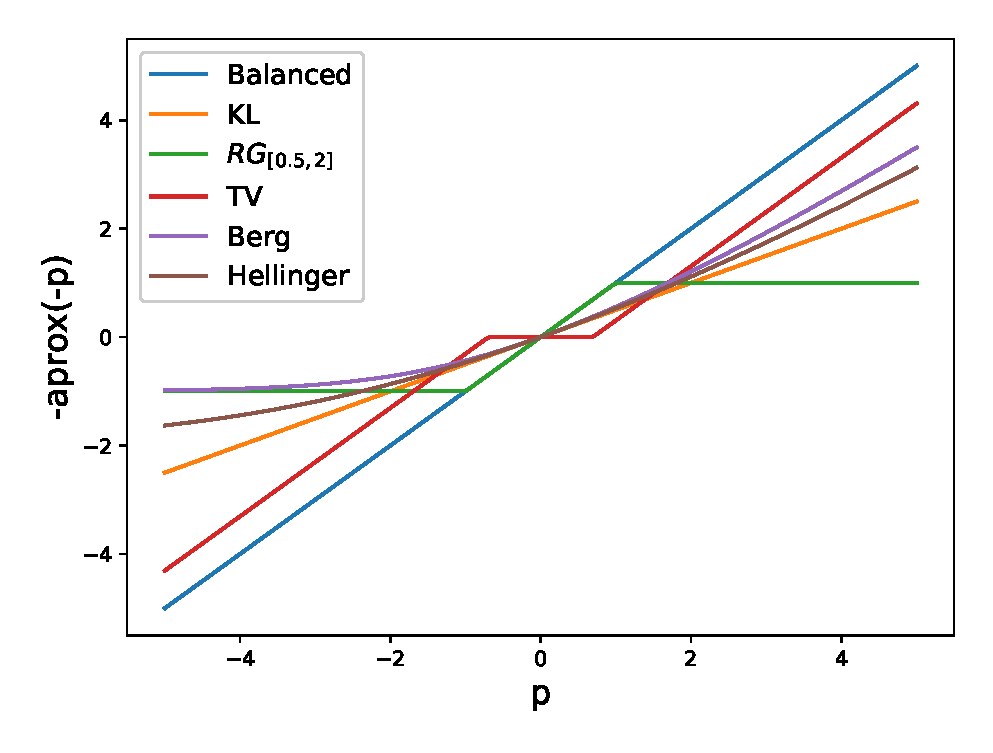
\includegraphics[width=.5\linewidth]{images/fig_aprox_5}
	\resizebox{!}{5cm}{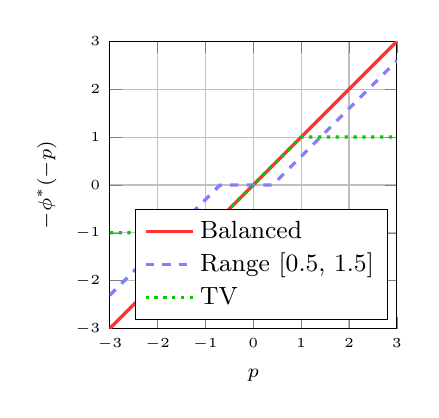
\begin{tikzpicture}
\iffalse
import sys
import numpy as np
p = np.linspace(-3, 3, 121)
a, b = 0.5, 1.5
eps, rho = 1, 1

# Range
range = p.copy()
range[p < eps * np.log(a)] -= eps * np.log(a)
range[(p >= eps * np.log(a)) * (p <= eps * np.log(b))] = 0
range[p > eps * np.log(b)] -= eps * np.log(b)

# TV
tv = p.copy()
tv[p < -rho] = -rho
tv[p > rho] = rho

values = np.stack((p, p, range, tv)).T
np.savetxt(sys.stdout, values, fmt="%.3f")
\fi

    \pgfplotstableread{
    p balanced range tv
    -3.000 -3.000 -2.307 -1.000
    -2.950 -2.950 -2.257 -1.000
    -2.900 -2.900 -2.207 -1.000
    -2.850 -2.850 -2.157 -1.000
    -2.800 -2.800 -2.107 -1.000
    -2.750 -2.750 -2.057 -1.000
    -2.700 -2.700 -2.007 -1.000
    -2.650 -2.650 -1.957 -1.000
    -2.600 -2.600 -1.907 -1.000
    -2.550 -2.550 -1.857 -1.000
    -2.500 -2.500 -1.807 -1.000
    -2.450 -2.450 -1.757 -1.000
    -2.400 -2.400 -1.707 -1.000
    -2.350 -2.350 -1.657 -1.000
    -2.300 -2.300 -1.607 -1.000
    -2.250 -2.250 -1.557 -1.000
    -2.200 -2.200 -1.507 -1.000
    -2.150 -2.150 -1.457 -1.000
    -2.100 -2.100 -1.407 -1.000
    -2.050 -2.050 -1.357 -1.000
    -2.000 -2.000 -1.307 -1.000
    -1.950 -1.950 -1.257 -1.000
    -1.900 -1.900 -1.207 -1.000
    -1.850 -1.850 -1.157 -1.000
    -1.800 -1.800 -1.107 -1.000
    -1.750 -1.750 -1.057 -1.000
    -1.700 -1.700 -1.007 -1.000
    -1.650 -1.650 -0.957 -1.000
    -1.600 -1.600 -0.907 -1.000
    -1.550 -1.550 -0.857 -1.000
    -1.500 -1.500 -0.807 -1.000
    -1.450 -1.450 -0.757 -1.000
    -1.400 -1.400 -0.707 -1.000
    -1.350 -1.350 -0.657 -1.000
    -1.300 -1.300 -0.607 -1.000
    -1.250 -1.250 -0.557 -1.000
    -1.200 -1.200 -0.507 -1.000
    -1.150 -1.150 -0.457 -1.000
    -1.100 -1.100 -0.407 -1.000
    -1.050 -1.050 -0.357 -1.000
    -1.000 -1.000 -0.307 -1.000
    -0.950 -0.950 -0.257 -0.950
    -0.900 -0.900 -0.207 -0.900
    -0.850 -0.850 -0.157 -0.850
    -0.800 -0.800 -0.107 -0.800
    -0.750 -0.750 -0.057 -0.750
    -0.700 -0.700 -0.007 -0.700
    -0.650 -0.650 0.000 -0.650
    -0.600 -0.600 0.000 -0.600
    -0.550 -0.550 0.000 -0.550
    -0.500 -0.500 0.000 -0.500
    -0.450 -0.450 0.000 -0.450
    -0.400 -0.400 0.000 -0.400
    -0.350 -0.350 0.000 -0.350
    -0.300 -0.300 0.000 -0.300
    -0.250 -0.250 0.000 -0.250
    -0.200 -0.200 0.000 -0.200
    -0.150 -0.150 0.000 -0.150
    -0.100 -0.100 0.000 -0.100
    -0.050 -0.050 0.000 -0.050
    0.000 0.000 0.000 0.000
    0.050 0.050 0.000 0.050
    0.100 0.100 0.000 0.100
    0.150 0.150 0.000 0.150
    0.200 0.200 0.000 0.200
    0.250 0.250 0.000 0.250
    0.300 0.300 0.000 0.300
    0.350 0.350 0.000 0.350
    0.400 0.400 0.000 0.400
    0.450 0.450 0.045 0.450
    0.500 0.500 0.095 0.500
    0.550 0.550 0.145 0.550
    0.600 0.600 0.195 0.600
    0.650 0.650 0.245 0.650
    0.700 0.700 0.295 0.700
    0.750 0.750 0.345 0.750
    0.800 0.800 0.395 0.800
    0.850 0.850 0.445 0.850
    0.900 0.900 0.495 0.900
    0.950 0.950 0.545 0.950
    1.000 1.000 0.595 1.000
    1.050 1.050 0.645 1.000
    1.100 1.100 0.695 1.000
    1.150 1.150 0.745 1.000
    1.200 1.200 0.795 1.000
    1.250 1.250 0.845 1.000
    1.300 1.300 0.895 1.000
    1.350 1.350 0.945 1.000
    1.400 1.400 0.995 1.000
    1.450 1.450 1.045 1.000
    1.500 1.500 1.095 1.000
    1.550 1.550 1.145 1.000
    1.600 1.600 1.195 1.000
    1.650 1.650 1.245 1.000
    1.700 1.700 1.295 1.000
    1.750 1.750 1.345 1.000
    1.800 1.800 1.395 1.000
    1.850 1.850 1.445 1.000
    1.900 1.900 1.495 1.000
    1.950 1.950 1.545 1.000
    2.000 2.000 1.595 1.000
    2.050 2.050 1.645 1.000
    2.100 2.100 1.695 1.000
    2.150 2.150 1.745 1.000
    2.200 2.200 1.795 1.000
    2.250 2.250 1.845 1.000
    2.300 2.300 1.895 1.000
    2.350 2.350 1.945 1.000
    2.400 2.400 1.995 1.000
    2.450 2.450 2.045 1.000
    2.500 2.500 2.095 1.000
    2.550 2.550 2.145 1.000
    2.600 2.600 2.195 1.000
    2.650 2.650 2.245 1.000
    2.700 2.700 2.295 1.000
    2.750 2.750 2.345 1.000
    2.800 2.800 2.395 1.000
    2.850 2.850 2.445 1.000
    2.900 2.900 2.495 1.000
    2.950 2.950 2.545 1.000
    3.000 3.000 2.595 1.000
    }\datatable
          
  
  \begin{axis}[width=.5\textwidth,
              grid=both,ymin=-3, ymax=3, xmin=-3, xmax=3,
      %title={\scriptsize We run NumPy, PyTorch and KeOps on a RTX 2080 Ti GPU.},
              xlabel={\scriptsize $p$}, 
              ylabel={\scriptsize $-\aprox{\phi^*}(-p)$}, 
              xtick={-3,-2,-1,0,1,2,3},
              %xticklabels={100,1k,10k,100k,1M},
              ytick={-3,-2,-1,0,1,2,3},
              %yticklabels={1\,ms,10\,ms,100\,ms,1\,s,10\,s},
              %xmode=log, ymode=log,
              legend pos = south east,
              %x post scale=1.7,
              grid=major,
            legend cell align={left},
            axis background/.style={fill=white},
            label style={font=\tiny},
            tick label style={font=\tiny},
            axis equal image,]
      \addplot[red!80, very thick,] table[x=p,y=balanced]  {\datatable};
      \addplot[blue!50, very thick, dashed] table[x=p,y=range]  {\datatable};
      \addplot[green!80!black, very thick, dotted] table[x=p,y=tv]  {\datatable};
      \addlegendentry{{\small Balanced}}
      \addlegendentry{{\small Range [0.5, 1.5]}}
      \addlegendentry{{\small TV}}
  \end{axis}
  \end{tikzpicture}}
	\quad
	\resizebox{!}{5cm}{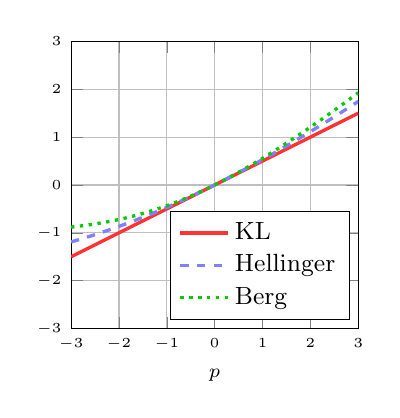
\begin{tikzpicture}
\iffalse
import sys
import numpy as np
from scipy.special import lambertw as W

p = np.linspace(-3, 3, 121)
a, b = 0.5, 1.5
eps, rho = 1, 1

# KL
kl = p * (rho / (rho + eps))

# Hellinger
hellinger = np.real(2 * eps * W((rho/eps) * np.exp((rho + p/2) / eps)) - 2*rho)

# Berg
berg = np.real(eps * W((rho/eps) * np.exp((rho + p) / eps)) - rho)

values = np.stack((p, kl, hellinger, berg)).T
np.savetxt(sys.stdout, values, fmt="%.3f")
\fi

    \pgfplotstableread{
    p balanced range tv
    -3.000 -1.500 -1.191 -0.880
    -2.950 -1.475 -1.176 -0.875
    -2.900 -1.450 -1.161 -0.869
    -2.850 -1.425 -1.147 -0.863
    -2.800 -1.400 -1.132 -0.857
    -2.750 -1.375 -1.116 -0.850
    -2.700 -1.350 -1.101 -0.844
    -2.650 -1.325 -1.085 -0.837
    -2.600 -1.300 -1.070 -0.830
    -2.550 -1.275 -1.054 -0.822
    -2.500 -1.250 -1.037 -0.815
    -2.450 -1.225 -1.021 -0.807
    -2.400 -1.200 -1.005 -0.798
    -2.350 -1.175 -0.988 -0.790
    -2.300 -1.150 -0.971 -0.781
    -2.250 -1.125 -0.954 -0.772
    -2.200 -1.100 -0.937 -0.762
    -2.150 -1.075 -0.919 -0.753
    -2.100 -1.050 -0.902 -0.743
    -2.050 -1.025 -0.884 -0.732
    -2.000 -1.000 -0.866 -0.722
    -1.950 -0.975 -0.848 -0.710
    -1.900 -0.950 -0.829 -0.699
    -1.850 -0.925 -0.811 -0.687
    -1.800 -0.900 -0.792 -0.675
    -1.750 -0.875 -0.773 -0.663
    -1.700 -0.850 -0.754 -0.650
    -1.650 -0.825 -0.735 -0.637
    -1.600 -0.800 -0.715 -0.623
    -1.550 -0.775 -0.695 -0.610
    -1.500 -0.750 -0.676 -0.595
    -1.450 -0.725 -0.656 -0.581
    -1.400 -0.700 -0.635 -0.566
    -1.350 -0.675 -0.615 -0.550
    -1.300 -0.650 -0.594 -0.535
    -1.250 -0.625 -0.574 -0.519
    -1.200 -0.600 -0.553 -0.502
    -1.150 -0.575 -0.532 -0.485
    -1.100 -0.550 -0.511 -0.468
    -1.050 -0.525 -0.489 -0.451
    -1.000 -0.500 -0.468 -0.433
    -0.950 -0.475 -0.446 -0.415
    -0.900 -0.450 -0.424 -0.396
    -0.850 -0.425 -0.402 -0.377
    -0.800 -0.400 -0.379 -0.358
    -0.750 -0.375 -0.357 -0.338
    -0.700 -0.350 -0.334 -0.318
    -0.650 -0.325 -0.311 -0.297
    -0.600 -0.300 -0.288 -0.276
    -0.550 -0.275 -0.265 -0.255
    -0.500 -0.250 -0.242 -0.234
    -0.450 -0.225 -0.219 -0.212
    -0.400 -0.200 -0.195 -0.190
    -0.350 -0.175 -0.171 -0.167
    -0.300 -0.150 -0.147 -0.144
    -0.250 -0.125 -0.123 -0.121
    -0.200 -0.100 -0.099 -0.097
    -0.150 -0.075 -0.074 -0.074
    -0.100 -0.050 -0.050 -0.049
    -0.050 -0.025 -0.025 -0.025
    0.000 0.000 0.000 0.000
    0.050 0.025 0.025 0.025
    0.100 0.050 0.050 0.051
    0.150 0.075 0.076 0.076
    0.200 0.100 0.101 0.102
    0.250 0.125 0.127 0.129
    0.300 0.150 0.153 0.155
    0.350 0.175 0.179 0.182
    0.400 0.200 0.205 0.210
    0.450 0.225 0.231 0.237
    0.500 0.250 0.258 0.265
    0.550 0.275 0.284 0.293
    0.600 0.300 0.311 0.321
    0.650 0.325 0.338 0.350
    0.700 0.350 0.365 0.379
    0.750 0.375 0.392 0.408
    0.800 0.400 0.419 0.437
    0.850 0.425 0.447 0.467
    0.900 0.450 0.474 0.497
    0.950 0.475 0.502 0.527
    1.000 0.500 0.530 0.557
    1.050 0.525 0.558 0.588
    1.100 0.550 0.586 0.619
    1.150 0.575 0.614 0.650
    1.200 0.600 0.643 0.681
    1.250 0.625 0.671 0.712
    1.300 0.650 0.700 0.744
    1.350 0.675 0.729 0.776
    1.400 0.700 0.758 0.808
    1.450 0.725 0.787 0.840
    1.500 0.750 0.816 0.873
    1.550 0.775 0.845 0.905
    1.600 0.800 0.875 0.938
    1.650 0.825 0.904 0.971
    1.700 0.850 0.934 1.005
    1.750 0.875 0.964 1.038
    1.800 0.900 0.993 1.072
    1.850 0.925 1.023 1.105
    1.900 0.950 1.054 1.139
    1.950 0.975 1.084 1.174
    2.000 1.000 1.114 1.208
    2.050 1.025 1.145 1.242
    2.100 1.050 1.175 1.277
    2.150 1.075 1.206 1.312
    2.200 1.100 1.237 1.347
    2.250 1.125 1.268 1.382
    2.300 1.150 1.299 1.417
    2.350 1.175 1.330 1.453
    2.400 1.200 1.362 1.488
    2.450 1.225 1.393 1.524
    2.500 1.250 1.424 1.560
    2.550 1.275 1.456 1.596
    2.600 1.300 1.488 1.632
    2.650 1.325 1.520 1.668
    2.700 1.350 1.552 1.705
    2.750 1.375 1.584 1.741
    2.800 1.400 1.616 1.778
    2.850 1.425 1.648 1.815
    2.900 1.450 1.680 1.852
    2.950 1.475 1.713 1.889
    3.000 1.500 1.745 1.926
    }\datatable
          
  
  \begin{axis}[width=.5\textwidth,grid=both,ymin=-3, ymax=3, xmin=-3, xmax=3,
      %title={\scriptsize We run NumPy, PyTorch and KeOps on a RTX 2080 Ti GPU.},
              xlabel={\scriptsize $p$}, 
              %ylabel={\scriptsize $-\aprox^\epsilon_{\phi^*}(-p)$}, 
              xtick={-3,-2,-1,0,1,2,3},
              %xticklabels={100,1k,10k,100k,1M},
              ytick={-3,-2,-1,0,1,2,3},
              %yticklabels={1\,ms,10\,ms,100\,ms,1\,s,10\,s},
              %xmode=log, ymode=log,
              legend pos = south east,
              %x post scale=1.7,
              grid=major,
            legend cell align={left},
            axis background/.style={fill=white},
            label style={font=\tiny},
            tick label style={font=\tiny},
            axis equal image,]
      \addplot[red!80, very thick,] table[x=p,y=balanced]  {\datatable};
      \addplot[blue!50, very thick, dashed] table[x=p,y=range]  {\datatable};
      \addplot[green!80!black, very thick, dotted] table[x=p,y=tv]  {\datatable};
      \addlegendentry{{\small KL}}
      \addlegendentry{{\small Hellinger}}
      \addlegendentry{{\small Berg}}
  \end{axis}
  \end{tikzpicture}}
	\caption{Display of the 1-Lipschitz operator $p \mapsto -\aprox{\phi^*}(-p)$ in the six major settings of Table~\ref{tab-entropies-aprox}, using $\epsilon=1$ and $\rho=1$.}
	\label{fig-aprox}
	%\end{figure}
	\vspace*{.7cm}
	
	\newcommand{\myfigE}[1]{\includegraphics[height=.14\linewidth]{images/compare_entropy/comparison_entropy_#1-c}}
	
	
	
	%\begin{figure}
	\centering
	\begin{tabular}{c@{\hspace{1mm}}c@{\hspace{1mm}}c@{\hspace{1mm}}}%
		\myfigE{reference} &
		\myfigE{Balanced} &
		\myfigE{KullbackLeibler} \\[-1mm]
		Inputs $(\al,\be)$ & $\iota_{(=)}$ & $10^{-1} * \KL$ \\[1mm]
		\myfigE{TotalVariation} &
		\myfigE{Range} &
		\myfigE{PowerEntropy} \\[-1mm]
		$10^{-1} * \TV$ & $\RG_{[0.7, 1.3]}$ & $10^{-1} * \text{Berg}$
	\end{tabular}
	\caption{Display of optimal marginals $(\textcolor{myred2}{\pi_1},\textcolor{myblue2}{\pi_2})$ depending on $\phi$. 
		The inputs $(\textcolor{myblue1}{\al},\textcolor{myred1}{\be})$ are 1D.
		Measures $(\textcolor{myblue1}{\al},\textcolor{myred1}{\be})$ and $(\textcolor{myred2}{\pi_1},\textcolor{myblue2}{\pi_2})$ are respectively plotted as dashed lines and filled colorings. 
		We use a regularization $\sqrt{\epsilon}=\sqrt{10^{-3}}$ on $[0,1]$.}
	\label{fig-comp-ent}
	%\end{figure}
	\vspace*{.7cm}
	
	\newcommand{\myfig}[1]{\includegraphics[width=.23\linewidth]{images/compare_reach/comparison_#1-c}}
	%\begin{figure}
	\centering
	\begin{tabular}{@{}c@{\hspace{1mm}}c@{\hspace{1mm}}c@{\hspace{1mm}}c@{\hspace{1mm}}c@{}}
		\rotatebox{90}{\small $\D_\phi=\rho\KL$} & \myfig{KullbackLeibler_reach001} & \myfig{KullbackLeibler_reach003} & \myfig{KullbackLeibler_reach013} & \myfig{KullbackLeibler_reach05} \\
		\rotatebox{90}{\small $\D_\phi=\rho\TV$\;\;} & \myfig{TotalVariation_reach001} & \myfig{TotalVariation_reach003} & \myfig{TotalVariation_reach013} & \myfig{TotalVariation_reach05} \\
		& $\rho=0.01$ & $\rho=0.03$ & $\rho=0.13$ & $\rho=0.5$
	\end{tabular}
	\caption{Display of marginals $(\textcolor{myred2}{\pi_1},\textcolor{myblue2}{\pi_2})$ depending on parameter $\rho$.
		We use the same inputs $(\textcolor{myblue1}{\al},\textcolor{myred1}{\be})$ from Figure~\ref{fig-comp-ent}. 
		First line corresponds to $\rho\KL$ and the second to $\rho\TV$.}
	\label{fig-impact-reach}
\end{minipage}
\end{figure}


\paragraph{Overview.}
%Figure~\ref{fig-aprox} displays $\aprox{\phi^*}$ for all aforementioned examples.
%We refer to Remark~\ref{rem-comment-sink} on its role of "dampening" balanced potentials.
%\begin{remark}\label{rem-comment-sink}
	We give an informal interpretation of Sinkhorn iterations for different divergences based on Proposition~\ref{prop-optimality-prox}, to illustrate the role of $\aprox{\phi^*}$.
	Optimality conditions have a compositional structure.
	Operators $(\Ss_\al,\Ss_\be)$ characterize optimal \emph{balanced} potentials as fixed points, and $\aprox{\phi^*}$ updates such fixed point by \emph{saturating} ($\D_\phi=\TV$) or \emph{dampening} ($\D_\phi=\KL$) dual potentials, see Figure~\ref{fig-aprox}.
	It indirectly impacts the plan via Equation~\eqref{eq-implicit-plan} by blocking or reducing transportation, see Figure~\ref{fig-impact-reach}.
%\end{remark}


Figure~\ref{fig-comp-ent} displays the impact of $\phi$ on the optimal plan $\pi$.
Here marginals $(\pi_1, \pi_2)$ are compared to the input marginals $(\al,\be)$.
Informally speaking, $\TV$ has 'sharp' marginals, i.e. it either transport s.t. $\pi_1(x)=\al(x)$ or destroys mass s.t. $\pi_1(x)=0$.
Marginals with $\KL$ are 'smooth' in the sense that it progressively transitions between transportation and destruction as $\C(x,y)$ increases.
Marginals for $\RG_{[a,b]}$ are less interpretable due to the box constraint, but we see that $\tfrac{\d\pi_1}{\d\al}\in\{a,b\}$.
The result of Berg entropy is similar to $\KL$, probably because they are both power entropies.
%
%\todo{Est-ce qu'on devrait supprimer ce paragraphe non mathématique ?}
%One sees that the marginals for $\KL$ have full support and that the density dampens as the distance between supports increases. For $\TV$ the density either matches the input or cancels out. The Range entropy is less intuitive due to the box constraint, the ratio of the density being equal to either one bound of the box or the other.
%The Berg entropy is represented here as an instance of the family of power entropies which includes the $\KL$, whence their similar behaviours.


Figure~\ref{fig-impact-reach} shows the impact of the parameter $\rho$ on $(\pi_1,\pi_2)$ (see Remark~\ref{rem-param-rho}). 
It illustrates that $\rho$ acts as a characteristic radius beyond which it is preferable to destroy mass than transport it. 
This phenomenon is sharp in the case of $\TV$ (it is known when $\epsilon=0$ that $\spt(\pi)\subset\{(x,y), \C(x,y)\leq 2\rho\}$) while there is a smooth dampening as $\C$ increases for $\KL$.


%
%\newcommand{\myfig}[1]{\includegraphics[width=.23\linewidth]{images/compare_reach/comparison_#1-c}}
%\begin{figure}
%	\centering
%	\begin{tabular}{@{}c@{\hspace{1mm}}c@{\hspace{1mm}}c@{\hspace{1mm}}c@{\hspace{1mm}}c@{}}
%		\rotatebox{90}{\small $\D_\phi=\rho\KL$} & \myfig{KullbackLeibler_reach001} & \myfig{KullbackLeibler_reach003} & \myfig{KullbackLeibler_reach013} & \myfig{KullbackLeibler_reach05} \\
%		\rotatebox{90}{\small $\D_\phi=\rho\TV$\;\;} & \myfig{TotalVariation_reach001} & \myfig{TotalVariation_reach003} & \myfig{TotalVariation_reach013} & \myfig{TotalVariation_reach05} \\
%		& $\rho=0.1$ & $\rho=0.03$ & $\rho=0.13$ & $\rho=0.5$
%	\end{tabular}
%	\caption{Display of the impact of the reach parameter $\rho$ on the marginals $(\textcolor{myred2}{\pi_1},\textcolor{myblue2}{\pi_2})$ given the same inputs $(\textcolor{myblue1}{\al},\textcolor{myred1}{\be})$ from Figure~\ref{fig-comp-ent}. First line corresponds to $\rho\KL$ and the second to $\rho\TV$.}
%	\label{fig-impact-reach}
%\end{figure}


\begin{table}
	\centering
	\def\arraystretch{1.2}
	\begin{adjustbox}{center}
		\begin{tabular}{|c@{}c@{\hspace{2mm}}c@{}c|}
			\hline
			Setting & Parameters & $\phi(p)$ & $-\aprox{\phi^*}(-p)$\\
			\hline
			Balanced & None & $0$ if $p=1$, $+\infty$ otherwise & $p$ \\
			Range & $0 \leq a \leq 1 \leq b$ & $0$ if $p \in [a, b]$, $+\infty$ otherwise &
			$\text{Soft-Thresh}_{\epsilon \log a}^{\epsilon \log b}(p)$ \\
			TV & $\rho > 0$ & $\rho\, |p-1|$ & $\text{Clamp}_{[-\rho, +\rho]}(p)$  \\
			KL & $\rho > 0$ & $\rho\, (p \log p - p + 1)$ & $\tfrac{\rho}{\rho+\epsilon}\, p$ \\
			Hellinger & $\rho > 0$ & $4 \rho\, (1 + (p-1)/2 - \sqrt{p})$ &  $2 \epsilon W(\tfrac{\rho}{\epsilon} \exp(\tfrac{\rho+p/2}{\epsilon})) - 2\rho $ \\
			Berg & $\rho > 0$ & $\rho\, (p - 1 - \log p)$ & $\epsilon W(\tfrac{\rho}{\epsilon} \exp(\tfrac{\rho+p}{\epsilon})) - \rho$ \\
			\hline
		\end{tabular}
	\end{adjustbox}
	\caption{Summary of the information that is required to implement
		the generalized Sinkhorn algorithm in six common settings.
	}
	\label{tab-entropies-aprox}
\end{table}





%%%%%%%%%%%%%%%%%%%%%%%%%%%%%%
\subsection{Convergence analysis and compactness of potentials}
\label{sec-convergence}

For discrete measures, alternate maximization is known to converge to maximizers for smooth problems~\cite{tseng2001convergence}, 
%
but convergence speeds known in the litterature depend on the number of samples.
Until now, there was no proof for general (continuous) measures.
%
In this section, we work over the \emph{infinite dimensional} space $\Mmp(\Xx)$ to overcome these limitations.
We prove linear convergence of the unbalanced Sinkhorn algoritm in full generality in Theorem~\ref{thm-cv-sink-compact} which is the main result of this section.


%%%%%%%%%%%%%%%%%%%%%%%%%%%%%%%%%%%%%%%%%%%%%%%%%%%%%%%%%%%%
\subsubsection{General convergence result}

Theorem~\ref{thm-cv-sink-compact} states convergence of Sinkhorn iterates, provided they remain in a compact subset of $\Cc(\Xx)^2$.
%
We then prove that this compactness hypothesis holds in a variety of settings, including Section~\ref{sec-exmp-f-div}.
A first setting studied in Section~\ref{subsubsec-convergence-compact} assumes $\phi^*$ is strictly convex, and holds in wide generality.
%A first case studied in Section~\ref{subsubsec-convergence-compact} is the one of strictly convex entropies that can be studied in full generality. 
The settings of balanced OT, TV and Range are convex but not strictly. They are treated separately in Section~\ref{sec-compact-balanced-tv-range}.

\begin{theorem}[The Sinkhorn algorithm solves the $\OTb$ problem]\label{thm-cv-sink-compact}
If the cost $\C$ is $\gamma$-Lipschitz, and if the dual program~\eqref{eq-dual-unb} can be restricted to a compact subset of $\Cc(\Xx)^2$, then there exists an optimal pair of dual potentials and the Sinkhorn algorithm converges towards a pair of optimal potentials.
%
In particular we have convergence for all settings of Section~\ref{sec-exmp-f-div}.
\end{theorem}

\begin{proof}
Consider a sequence $(\f_n,\g_n)_n$ approaching $\OT(\al,\be)=\sup\Ff$. 
Compactness in $\Cc(\Xx)$ allows to extract $(\f_{n_k},\g_{n_k})\rightarrow(\f,\g)$, where $(\f,\g)\in\Cc(\Xx)^2$ are optimal, i.e. $\OT(\al,\be)=\Ff(\f,\g)$.

Now write $(\f_t,\g_t)$ the Sinkhorn iterates~\eqref{eq-sinkhorn-iter-1} for some $\f_0\in\Cc(\Xx)$.
Iterates $(\f_t,\g_t)$ are $\gamma$-Lipschitz (Proposition~\ref{lem-smin-cost-regular}), thus equicontinuous on $\Xx$. 
Furthermore, non-expansivity of $\Aa\Ss$ (Propositions~\ref{lem-smin-lipschitz-func} and~\ref{prop-nonexp}) implies $\norm{\f_t - \f}_\infty\leq\norm{\f_{0} - \f}_\infty$.
Since $\f\in\Cc(\Xx)$ and $\Xx$ compact, then $\norm{\f}_\infty < \infty$. 
Thus $\norm{\f_t}_\infty \leq\norm{\f_{0} - \f}_\infty + \norm{\f}_\infty$.

Ascoli-Arzela theorem holds and Sinkhorn iterates $(\f_t,\g_t)_t$ are a compact sequence in $\Cc(\Xx)$.
Take any subsequence $\f_{t_k}\rightarrow \f_*$, and $\eta >0$. There exists $k$ such that $\norm{\f_{k} - \f_*}_\infty < \eta$. 
Non-expansivity of $\Aa\Ss$ implies again that $\forall t\geq k,\, \norm{\f_{t} - \f_*}_\infty\leq\norm{\f_{k} - \f_*}_\infty < \eta$.
The same fact holds for $(\g_t)$
This inequality is the definition of the convergence of $(\f_t)$.
Thus any subsequence verifies $\f_{t_k}\rightarrow\f_*$ and then $\f_t\rightarrow\f_*$. 
Thus Sinkhorn iterates converge towards $(\f_*,\g_*)$ and are fixed point of the Sinkhorn maps.
Thus they are optimal (Proposition~\ref{prop-cns-optimality}).

Thanks to Lemmas~(\ref{lem-compact-dual},\ref{lem-compact-balanced},\ref{lem-compact-tv},\ref{lem-compact-range}), we can restrict Problem~\eqref{eq-dual-unb} to a compact set, hence the convergence for all settings of Section~\ref{sec-exmp-f-div}.
\end{proof}

Theorem~\ref{thm-cv-sink-compact} reduces proofs of \emph{convergence} to proofs of \emph{compactness} of the sequence $(\f_n,\g_n)$. 
We detail these results in Sections~\ref{subsubsec-convergence-compact} and~\ref{sec-compact-balanced-tv-range}.
We give before a sufficient condition of convergence when $\aprox{\phi^*}$ is contractive.
It holds for $\KL$ and some Power entropies (see Proposition~\ref{prop-aprox-power-ent}).
%but first give a sufficient condition on the convergence of the Sinkhorn algorithm when the aprox operator is contractive. All families of strictly convex entropy functions shown in Section~\ref{sec-exmp-f-div} induce proximity operators that are contractions on compact sets, and can thus benefit from this direct proof.

\begin{proposition}\label{prop-contractive-sink}
If $\aprox{\phi^*}$ is a contraction on compact sets w.r.t.~$\norm{\cdot}_\infty$ and if $\C$ is $\gamma$-Lipschitz, then the Sinkhorn algorithm converges linearly towards a unique fixed point w.r.t $\norm{\cdot}_\infty$.
\end{proposition}

\begin{proof}
The Softmin is non-expansive (Lemma~\ref{lem-smin-lipschitz-func}) and Lemma~\ref{lem-smin-cost-regular} gives the continuity of $\Ss_\al(\f)$ and $\Ss_\be(g)$, which are bounded on compact sets. Thus composing with $\aprox{\phi^*}$ gives a contractive mapping with respect to $\norm{.}_\infty$.
\end{proof}

\begin{remark}\label{rem-cv-balanced-sink}
	A similar contraction theorem holds for \emph{balanced} OT.
	The Birkhoff-Hopf theorem from non-linear Perron-Frobenius theory~\cite{lemmens2012nonlinear} states that $(\Ss_\al,\Ss_\be)$ are contractive w.r.t. the Hilbert pseudo-norm.
\end{remark}
%Note that .
%In this case, the Birkhoff theorem of non-linear Perron Frobenius theory allows us to show that the Softmin is contractive with respect to the Hilbert metric ~\cite{lemmens2012nonlinear}.


%%%%%%%%%%%%%%%%%%%%%%%%%%%%%%%%%%%%%%%%%%%%%%%%%%%%%%%%%%%%
\subsubsection{Lemmas on compactness of potentials}
\label{subsubsec-lemma-factor-compact}

This section reduces the proof of compactness in two parts thanks to the structure of $\Ff(\f,\g)$.
Lemma~\ref{lem-uniq-tensor-sum} below states $(\f,\g)$ are optimal up to translations $(\f+\lambda,\g-\lambda)$ for $\lambda\in\R$.
This invariance allows to assume $\f(x_0)=0$ for some $x_0\in\Xx$, and to build a compact set in Lemma~\ref{lem-compact-anchor}.
It then remains to prove that admissible translations $\lambda$ lie in a compact set, which is treated in Sections~\ref{subsubsec-convergence-compact} and~\ref{sec-compact-balanced-tv-range}.

\begin{lemma}[Uniqueness of the optimal dual pair]\label{lem-uniq-tensor-sum}
For any $(\al,\be)\in\Mmpp(\Xx)$, there is uniqueness of optimal potentials $(\f,\g)$ for the dual program~\eqref{eq-dual-unb} in the following sense: if there are two optimal solutions $(\f_1,\g_1)$ and $(\f_2,\g_2)$ then $\f_1\oplus\g_1 = \f_2\oplus\g_2$, $\alpha \otimes \beta$-a.e.. Thus, given optimal potentials $\f\oplus\g$, all other optimal ones can only be $\alpha \otimes \beta$-a.e. of the form $(\f + \lambda, \g-\lambda)$ for some $\lambda\in\R$.
\end{lemma}
%\begin{proof}
% Denote the dual functional~\eqref{eq-dual-unb} as $\mathcal{F}$ and assume  the existence of two couples of dual potentials $(f_1,g_1)$ and $(f_2,g_2)$ such that $ \mathcal{F}(f_1,g_1) = \mathcal{F}(f_2,g_2)$. Due to the optimality of potentials and the joint convexity of $\Ff$ we have that
% $\mathcal{F}(t f_1 + (1-t) f_2, t g_1 + (1-t) g_2) = t \mathcal{F}(f_1,g_1) + (1-t) \mathcal{F}(f_2,g_2)$.
%Because the function $h\mapsto -\dotp{\al\otimes\be}{e^{(h -\C)/\epsilon} }$ is strictly concave on the support of $\al\otimes\be$, the previous equality imposes
%\begin{multline}
% \dotp{\al\otimes\be}{e^{(t f_1 \oplus g_1 + (1-t) f_2 \oplus g_2 -\C)/\epsilon} } \\=  \dotp{\al\otimes\be}{te^{( f_1 \oplus g_1  -\C)/\epsilon}  + (1-t) e^{( f_2 \oplus g_2 -\C)/\epsilon} }\,,
%\end{multline}
%Again due to the strict convexity and because we integrate continuous functions against positive measures, we deduce a pointwise equality that $\alpha \otimes \beta$ a.e., one has
%$t (f_1(x)+g_1(y)) + (1-t)(f_2(x) + g_2(y)) = f_1(x)+g_1(y) = f_2(x) + g_2(y)$,
%which implies $f_1 \oplus g_1 = f_2 \oplus g_2$, $\alpha \otimes \beta$ a.e.
%\end{proof}
\begin{proof}
	Write $(\f_1,\g_1)$ and $(\f_2,\g_2)$ two optimal pairs for~\eqref{eq-dual-unb}, and define $\f_t=t\f_1 + (1-t)\f_2$ and $\g_t=t\g_1 + (1-t)\g_2$ with $t\in[0,1]$. Write
	\begin{align*}
		a_1 &= \dotp{\al}{-\phi^*(-\f_t)} + \dotp{\be}{-\phi^*(-\g_t)},\\
		a_2 &= \dotp{\al}{-t\phi^*(-\f_1) - (1-t)\phi^*(-\f_2)} + \dotp{\be}{-t\phi^*(-\g_1) - (1-t)\phi^*(-\g_2)},\\
		b_1 &= -\epsilon\dotp{\al\otimes\be}{e^{(\f_t\oplus\g_t-\C) / \epsilon} - 1},\\
		b_2 &= -\epsilon\dotp{\al\otimes\be}{t e^{(\f_1\oplus\g_1-\C) / \epsilon} + (1-t)e^{(\f_2\oplus\g_2-\C) / \epsilon} - 1}.
	\end{align*}
	By optimality and convexity of the problem one has $a_1 + b_1 = a_2 + b_2$ as well as $a_1\geq a_2$ and $b_1\geq b_2$, thus necessarily $a_1=a_2$ and $b_1=b_2$. In particular the equality $b_1=b_2$ is an integral against a positive measure whose integrand verifies pointwise $e^{(\f_t(x)\oplus\g_t(y)-\C) / \epsilon}\leq te^{(\f_1(x)\oplus\g_1(y)-\C) / \epsilon} + (1-t)e^{(\f_2(x)\oplus\g_2(y)-\C) / \epsilon}$, thus the inequaliy becomes a pointwise equality holding $\al\otimes\be$-a.e. Eventually, the strict convexity of the exponential yields $\al\otimes\be$-a.e. that $t (f_1(x)+g_1(y)) + (1-t)(f_2(x) + g_2(y)) = f_1(x)+g_1(y) = f_2(x) + g_2(y)$.
\end{proof}

We warn that not all $\lambda$ yield an optimal pair.
There exists a unique $\lambda$ for strictly convex $\phi^*$, while any $\lambda\in\R$ is optimal for balanced OT.
%The above lemma asserts that the possibly optimal potentials of the dual program are necessarily of the form $(\f + \lambda, \g-\lambda)$ -- but not all $\lambda$ yield an optimal pair. We prove in the following lemma that we can restrict the dual program to a set of functions which will be proved to be compact. It then remains to prove compactness with respect to $\lambda$, which is detailed in Sections~\ref{subsubsec-convergence-compact} and~\ref{sec-compact-balanced-tv-range}.


\begin{lemma}[Compact Anchoring of $(\f,\g)$]\label{lem-compact-anchor}
	Assume $\C$ is $\gamma$-Lipschitz, and define 
	$\Pp_{x_o} \eqdef \{ (\f,\g)\in\Aa\Ss_\be(\Cc(\Xx))\times\Aa\Ss_\al(\Cc(\Xx)),\, \f(x_0) = 0,\,\exists M\in\R,\, \norm{\f\oplus\g}_\infty \leq M \}$ 
	for some $x_0\in\Xx$.
	Then one can restrict the dual~\eqref{eq-dual-unb} as a supremum over $\Pp_{x_o}+\R \eqdef\{(\f + \lambda,\g-\lambda),\, (\f,\g)\in\Pp_{x_0},\, \lambda\in\R\}$.
	Furtermore the set $\Pp_{x_o}$ is relatively compact in $\Cc(\Xx)$.
\end{lemma}
\begin{proof}
	Optimality of $(\f,\g)$ is equivalent to have $(\f,\g)=(\Aa\Ss_\be(\g), \Aa\Ss_\al(\f))$ (Proposition~\ref{prop-cns-optimality}), hence the restriction to $\Aa\Ss_\be(\Cc(\Xx))\times\Aa\Ss_\al(\Cc(\Xx))$.
	Such potentials are $\gamma$-Lipschitz (Lemma~\ref{lem-smin-cost-regular}).
	
	We show that in $\Aa\Ss_\be(\Cc(\Xx))\times\Aa\Ss_\al(\Cc(\Xx))$, there exists $\tilde{M}$ s.t. $\norm{\f\oplus\g}_\infty \leq \tilde{M}$.
	Consider a sequence $(\f_n,\g_n)_n$ such that $\norm{\f_n\oplus\g_n}_\infty\rightarrow+\infty$. 
	We have $(\f_n,\g_n)\in\Cc(\Xx)$ with $\Xx$ compact, thus $\exists(x_n,y_n)\in\Xx^2,\,\norm{\f_n\oplus\g_n}_\infty=(\f_n\oplus\g_n)(x_n,y_n)$. 
	We have $(\f_n\oplus\g_n)(x_n,y_n)\rightarrow+\infty$. 
	Since $(\f_n,\g_n)$ are $\gamma$-Lipschitz, $\forall(x,y)\in\Xx^2,\, |(\f_n\oplus\g_n)(x_n,y_n) - (\f_n\oplus\g_n)(x,y)|\leq 2\gamma \text{diam}(\Xx)$, thus $\norm{\f_n\oplus\g_n}_\infty - 2\gamma \text{diam}(\Xx) \leq (\f_n\oplus\g_n)(x,y)$. 
	When $(x,y)\in\spt(\al)\times\spt(\be))$, $(\f_n\oplus\g_n)(x,y)\rightarrow+\infty$ and $\Ff(\f_n,\g_n)\rightarrow-\infty$.
	Similarly, if $(\f_n\oplus\g_n)(x_n,y_n)\rightarrow-\infty$ then $\Ff(\f_n,\g_n)\rightarrow-\infty$. 
	Hence we have $\norm{\f\oplus\g}_\infty \leq \tilde{M}$.
	
	Assume $\norm{\f\oplus\g}_\infty \leq \tilde{M}$.
	Potentials $(\f+\lambda,\g-\lambda)$ with $\lambda\in\R$ have the same bound. 
	Thus w.l.o.g. $\f(x_0)=0$ for some $x_0\in\Xx$. 
	Since $\f$ is $\gamma$-Lipschitz, we have $\norm{\f}_\infty \leq\gamma \text{diam}(\Xx)$ because $\f(x_0)=0$.
	Thus $\norm{\g}_\infty \leq \norm{\f} + \norm{\f\oplus\g}_\infty \leq \gamma \text{diam}(\Xx) + \tilde{M} = M.$
	Thus potentials in $E$ satisfy all properties.
	
	In $\Pp_{x_0}$ potentials are uniformly equicontinuous because $\norm{\f}_\infty,\norm{\g}\leq M$.
	Ascoli-Arzela theorem holds, and $\Pp_{x_0}$ is relatively compact in $\Cc(\Xx)$.
\end{proof}

%\begin{lemma}[Anchoring of the dual potentials]\label{lem-restrict-pot}
%If the cost $\C$ is $\gamma$-Lipschitz, the dual program~\eqref{eq-dual-unb} can be restricted to a subset of functions of $\Tt_\be(\Cc(\Xx))\times\Tt_\al(\Cc(\Xx))$ of the form $(\f+\lambda,\g-\lambda)$ with $\lambda\in\R$, such that $\f(x_0)=0$ for some $x_0\in\Xx$ and such that $(\f,\g)$ satisfies $\norm{\f}_\infty \leq M$ and $\norm{\g}_\infty \leq M$ for some finite $M\in\R_+$.
%\end{lemma}
%\begin{proof}
%Optimality of potentials is equivalent to be a fixed point of the Sinkhorn mapping (Proposition~\ref{prop-cns-optimality}), thus we can restrict to potentials in $E = \Tt_\be(\Cc(\Xx))\times\Tt_\al(\Cc(\Xx))$. Such potentials are $\gamma$-Lipschitz (Lemma~\ref{lem-smin-cost-regular}).
%
%We show that in $E$, $\norm{\f\oplus\g}_\infty \leq \tilde{M}$.
%Consider a sequence $(\f_n,\g_n)_n$ such that $\norm{\f\oplus\g}_\infty\rightarrow+\infty$. 
%We have $(\f_n,\g_n)\in\Cc(\Xx)$ with $\Xx$ compact, thus $\exists(x_n,y_n)\in\Xx^2,\,\norm{\f_n\oplus\g_n}_\infty=(\f_n\oplus\g_n)(x_n,y_n)$. 
%We have $(\f_n\oplus\g_n)(x_n,y_n)\rightarrow+\infty$. 
%Since $(\f_n,\g_n)$ are $\gamma$-Lipschitz, $\forall(x,y)\in\Xx^2,\, |(\f_n\oplus\g_n)(x_n,y_n) - (\f_n\oplus\g_n)(x,y)|\leq 2\gamma \text{diam}(\Xx)$, thus $\norm{\f_n\oplus\g_n}_\infty - 2\gamma \text{diam}(\Xx) \leq (\f_n\oplus\g_n)(x,y)$. 
%When $(x,y)\in\spt(\al)\times\spt(\be))$, $(\f_n\oplus\g_n)(x,y)\rightarrow+\infty$ and $\Ff(\f_n,\g_n)\rightarrow-\infty$.
%Similarly, if $(\f_n\oplus\g_n)(x_n,y_n)\rightarrow-\infty$ then $\Ff(\f_n,\g_n)\rightarrow-\infty$. 
%Hence we have $\norm{\f\oplus\g}_\infty \leq \tilde{M}$.
%
%Assume $\norm{\f\oplus\g}_\infty \leq \tilde{M}$.
%Potentials $(\f+\lambda,\g-\lambda)$ with $\lambda\in\R$ have the same bound. 
%Thus w.l.o.g. $\f(x_0)=0$ for some $x_0\in\Xx$. 
%Since $\f$ is $\gamma$-Lipschitz, we have $\norm{\f}_\infty \leq\gamma \text{diam}(\Xx)$ because $\f(x_0)=0$.
%Thus $\norm{\g}_\infty \leq \norm{\f} + \norm{\f\oplus\g}_\infty \leq \gamma \text{diam}(\Xx) + \tilde{M} = M.$
%Thus potentials in $E$ satisfy all properties.
%
%In $\Pp_{x_0}$ potentials are uniformly equicontinuous.
%Ascoli-Arzela theorem holds, and $\Pp_{x_0}$ is relatively compact in $\Cc(\Xx)$.
%\end{proof}
%
%In what follows we always consider such set of functions, because it is compact as stated below. 
%%The next lemma asserts that the set of potentials with an anchor point is compact. Thus it remains to prove that the set of such translated potentials that yields an optimal pair of potentials is compact.
%
%\begin{lemma}[Relative compactness of sets of anchored potentials]\label{lem-compact-anchor}
%Let $\C$ be a $\gamma$-lipschitz cost function. For any $(\al,\be)\in\Mmpp(\Xx)$ the sets
% $\Pp_{x_o} = \{ (\f,\g)\in\Tt_\be(\Cc(\Xx))\times\Tt_\al(\Cc(\Xx)),\, \f(x_0) = 0,\, \norm{\f\oplus\g}_\infty \leq M \} $
% are relatively compact in $\Cc(\Xx)$.
%\end{lemma}
%\begin{proof}
%Reusing the above proof of Lemma~\ref{lem-restrict-pot}, we get that for any $(\f,\g)\in\Pp_{x_0}$, the potentials $(\f,\g)$ are $\gamma$-Lipschitz and verify $\norm{\f}_\infty \leq \tilde{M}$ and $\norm{\g}_\infty \leq  \tilde{M}$. Thus $\f$ and $\g$ are both uniformly equicontinuous. The Ascoli-Arzela theorem applies, which gives that the set $\Pp_{x_0}$ is relatively compact in $\Cc(\Xx)$.
%\end{proof}


%%%%%%%%%%%%%%%%%%%%%%%%%%%%%%%%%%%%%%%%%%%%%%%%%%%%%%%%%%%%
\subsubsection{Compactness for strictly convex entropies}
\label{subsubsec-convergence-compact}

We prove compactness of potentials under two fairly general assumptions.

\begin{assumption}\label{as:1}
  The function $\phi^*$ is strictly convex.
\end{assumption}
\begin{assumption}\label{as:2}
  There exists a sequence $(x_n)_n \subset \text{\upshape dom}(\phi^*)$ and $s_n\in\partial\phi^*(x_n)$ such that $s_n$ converges either to zero or $+\infty$. 
\end{assumption}
The cases of $\KL$ and Power entropies mentioned Section~\ref{sec-exmp-f-div} satisfy those assumptions.
%The Kullback-Leibler and the power-entropies are the divergences mentioned in Section~\ref{sec-exmp-f-div} which verify both  assumptions.
%
%This property is fundamental to ensure existence and uniqueness of potentials, and prove the weak* differentiability of our optimal transport loss.
This setting ensures existence and uniqueness of optimal $(\f,\g)$, the latter being key for weak* differentiability of $\OTb$ and $\Sb$.
%
%We detail the need for those assumptions in Example~\ref{exmp-range2}, at the end of this Section.

\begin{lemma}[Restriction of the dual $\OTb$ problem to a compact set]\label{lem-compact-dual}
Let $\C$ be a $\gamma$-lipschitz cost function. Under Assumption~\ref{as:2}, the dual problem~\eqref{eq-dual-unb} can be restricted to a supremum over the compact set $\overline{\Pp_{x_0} + I}$ where
\begin{align*}
  \Pp_{x_0} + I = \{ (\f+\lambda,\g-\lambda),\, (\f,\g)\in\Pp_{x_0}, \lambda\in I \}
\end{align*}
with $I$ being a compact set. Furthermore, the compact interval $I$ only depends on $(m(\al),m(\be))$ in a neighborhood of $(\al,\be)$ and this dependency is continuous.
\end{lemma}

\begin{proof}
Lemma~\ref{lem-compact-anchor} applies, thus we consider potentials $(\f+\lambda,\g-\lambda)$ with $(\f,\g)\in\Pp_{x_0}$ (relatively compact) and $\lambda\in\R$.
It remains to prove that the dual program~\eqref{eq-dual-unb} is coercive w.r.t. $\lambda$.

Since $\phi^*$ is convex one has for any $q$ such that $-q\in\text{dom}(\phi^*)$ and $s\in\partial\phi^*(-q)$
\begin{align*}
  \dotp{\al}{-\phi^*(-\f-\lambda)} &\leq \dotp{\al}{-\phi^*(-q) +s(\f + \lambda-q)} \\
  &\leq m(\al) \big(  -\phi^*(-q) +s(\norm{\f}_\infty + \lambda-q) \big).
\end{align*}
From this and the similar inequality for $\be$, we deduce for any $(-q,-\tilde{q})\in\text{dom}(\phi^*)$ and $(s,\tilde{s})\in\partial\phi^*(-q)\times\partial\phi^*(-\tilde{q})$ that
%\begin{align*}
%  \dotp{\al}{-\phi^*(-\f - \lambda)} &+ \dotp{\be}{-\phi^*(-\g + \lambda)}\\
%  &\leq \big[m(\al)s - m(\be)\tilde{s}\big]\lambda \eqdef R(s, \tilde{s})\lambda\\
%   &\begin{array}{@{}l}+ m(\al)\big(-\phi^*(-q) + s(\norm{\f}_\infty -q) \big)\\ + m(\be)\big(-\phi^*(-\tilde{q}) + \tilde{s}(\norm{\g}_\infty -\tilde{q}) \big)\end{array} \Big\}\eqdef K.
%\end{align*}
\begin{align*}
\Ff(\f+\lambda,\g-\lambda)=\dotp{\al}{-\phi^*(-\f - \lambda)} &+ \dotp{\be}{-\phi^*(-\g + \lambda)}\leq  R(s, \tilde{s})\lambda + K,%(m(\al), m(\be), \norm{\f}_\infty, \norm{\g}_\infty, q, \tilde{q}, s, \tilde{s}),
\end{align*}
where $R(s, \tilde{s})\eqdef m(\al)s - m(\be)\tilde{s}$ and
\begin{align*}
	K \eqdef m(\al)\big(-\phi^*(-q) + s(\norm{\f}_\infty -q) \big)+ m(\be)\big(-\phi^*(-\tilde{q}) + \tilde{s}(\norm{\g}_\infty -\tilde{q}) \big).
\end{align*}
To be coercive in $\lambda$, we need to find points $(q_1,\tilde{q}_1)\in\text{dom}(\phi^*)^2$, $(s_1, \tilde{s}_1)\in\partial\phi^*(q_1)\times\partial\phi^*(\tilde{q}_1)$ and $(q_2,\tilde{q}_2)\in\text{dom}(\phi^*)^2$, $(s_2, \tilde{s}_2)\in\partial\phi^*(q_2)\times\partial\phi^*(\tilde{q}_2)$ such that $K<+\infty$ (it holds on $\text{dom}(\phi^*)$), such that $R(s_1,\tilde{s}_1) > 0$ and $R(s_2,\tilde{s}_2) < 0$. 
Assumption~\ref{as:2} proves it. 
We have $\partial\phi^*\subset\R_+$. 
If  $\exists s_n\in\partial\phi^*(x_n)$ with $s_n\rightarrow 0$, take $q_1\in\text{dom}(\phi^*)$ and $\tilde{q}_1=x_n$.
There exists $n_0$, such that $s_n$ is small enough for $n\geq n_0$ and $R(s_1, s_n)>0$. 
Similarly we find some $R(s_2, \tilde{s}_2)<0$. 
The same approach holds for $\partial\phi^*(x_n)\rightarrow +\infty$. 
Thus $\Ff(\f+\lambda,\g-\lambda)\rightarrow-\infty$ when $\lambda\rightarrow\pm\infty$ by taking either $R<0$ or $R>0$.

Note that $(R,K)$ depends continuously on $(m(\al),m(\be))$. Thus, on a neighbourhood of $(\al,\be)$, one still has $R(s_1, \tilde{s}_1) > 0$, $R(s_2, \tilde{s}_2) < 0$ and $|K|<\infty$.

Coercivity holds and $\lambda$ is in a compact interval $I$ that is constant in a neighborhood of $(\al,\be)$. 
Thus the optimal potentials can be taken in a set $\Pp_{x_0}+I$. 
The potentials inside this set remain equicontinuous and uniformly bounded. 
The Ascoli-Arzelà theorem applies and $\Pp_{x_0}+I$ is relatively compact in $\Cc(\Xx)$.
\end{proof}

Lemma~\ref{lem-compact-dual} and Assumptions~\ref{as:1} ensure existence and uniqueness of optimal $(\f,\g)$.
We now prove $(\f,\g)$ depend continuously in $(\al,\be)$, which is key for the weak* regularity of $\OTb$ studied in Section~\ref{sec-ot-prop}. 
%Note that under Assumption~\ref{as:1}, the dual~\eqref{eq-dual-unb} is strictly convex in $(\f,\g)$: there is uniqueness of the optimal pair.

\begin{proposition}[The dual potentials vary continuously with the input measures]
\label{prop-uniform-conv}
Let $\C$ be a $\gamma$-lipschitz cost function.
Let $\al_n \rightharpoonup \al$ and
$\be_n \rightharpoonup \be$ be weakly converging
sequences of measures in $\Mmpp(\Xx)$.
Write $(\f_n,\g_n)$ the (unique) sequence of optimal
potentials for $\OTb(\al_n,\be_n)$.

Under Assumptions~\ref{as:1} and \ref{as:2}, $\f_n$ and $\g_n$ converge uniformly towards the
unique pair of optimal potentials $(\f,\g)$ for $\OTb(\al,\be)$:
\begin{align*}
\big( \al_n \rightharpoonup \al, \,
\be_n \rightharpoonup \be
\big)\Longrightarrow
\big( \f_n \xrightarrow{\|\cdot\|_\infty} \f, \,
\g_n \xrightarrow{\|\cdot\|_\infty} \g
\big).
\end{align*}
\end{proposition}

\begin{proof}
  Thanks to Theorem~\ref{thm-cv-sink-compact}, for all $(\al_n,\be_n)$, $\exists !(\f_n,\g_n)$ optimal in $\OTb(\al_n,\be_n)$. 
  Applying Lemma~\ref{lem-compact-dual}, we assume $(\f_n,\g_n)\in\Pp_{x_0}+I_n$.
  The interval $I_n$ depends continuously in $(m(\al_n),m(\be_n))$ in a neighborhood of $(\al_n,\be_n)$. 
  Since $(\al_n,\be_n)\rightharpoonup(\al,\be)$ with $m(\al),m(\be)>0$,
  there exists $(-q_i, -\tilde{q}_i)\in\text{dom}(\phi^*)^2$, $(s_i,\tilde{s}_i)\in\partial\phi^*(-q_i)\times\partial\phi^*(-\tilde{q}_i)$, $\eta >0$ and $n_0$ such that for all $n \geq n_0$
\begin{gather*}
  0 < m(\al) -\eta < m(\al_n) < m(\al) +\eta \; \text{and} \; 0 < m(\be) -\eta < m(\be_n) < m(\be) +\eta\\
  \Rightarrow R_+ \eqdef (m(\al)-\eta)s_1 - (m(\be)+\eta)\tilde{s}_1 < R(s_1,\tilde{s}_1)<0,\\
   \Rightarrow R_- \eqdef (m(\al)+\eta)s_2 - (m(\be)-\eta)\tilde{s}_2 > R(s_1,\tilde{s}_1)>0,
\end{gather*}
where $R$ is defined in the proof of Lemma~\ref{lem-compact-dual}. 
Again, Assumption~\ref{as:2} guarantees that we find points in $\text{dom}(\phi^*)$, independent of $n$, such that $\forall n \geq n_0$, $R_+ <0$ and $R_- >0$. 
We then build a compact subset $\Pp_{x_0}+I$ with $I$ compact and independent of $n$ such that for all $n$, $(\f_n,\g_n)\in\Pp_{x_0}+I$.
Ascoli-Arzelà theorem holds.
   One  extracts a subsequence $(\f_{n_k},\g_{n_k})\rightarrow(\f,\g)$, where $(\f,\g)$ are unique optimal in $\OTb(\al,\be)$. 
   All subsequences converge to the same limit due to uniqueness of optimal potentials. 
   Hence we get $(\f_n,\g_n)\rightarrow(\f,\g)$.
\end{proof}

%%%%%%%%%%%%%%%%%%%%%%%%%%%%%%%%%%%%%%%%%%%%%%%%%%%%%%%%%%%%%%%%%%%%%%%%%%%%%%%%%%%%%%%%%%%%%%%%
\subsubsection{Compactness for Balanced, Total Variation and Range entropies}
\label{sec-compact-balanced-tv-range}

The settings of balanced, TV and Range OT do not satisfy Assumption~\ref{as:1}. 
We prove compactness below with Lemmas~(\ref{lem-compact-balanced},\ref{lem-compact-tv},\ref{lem-compact-range}) dedicated to each setting.
They guarantee Theorem~\ref{thm-cv-sink-compact} holds.
%We start with balanced transport, using a proof that is adapted from~\cite{berman2017sinkhorn}.
%Nevertheless, compactness holds and yields convergence of the Sinkhorn algorithm. 
%We provide the following three lemmas stating this property with their respective proofs. 

%Those lemmas guarantee that Theorem~\ref{thm-cv-sink-compact} holds and thus that Sinkhorn's algorithm converges even in those unfavorable settings.



\begin{lemma}[Balanced OT]\label{lem-compact-balanced}
In the setting of balanced OT where $\phi^*(x)=x$, the dual program can be restricted to the compact set $\Pp_{x_0}$.
\end{lemma}
\begin{proof}
Lemma~\ref{lem-compact-anchor} applies, thus we consider potentials $(\f+\lambda,\g-\lambda)$ with $(\f,\g)\in\Pp_{x_0}$ and $\lambda\in\R$.
In this setting $\Ff(\f+\lambda, \g-\lambda)=\Ff(\f,\g)$. This invariance allows us to quotient $\Cc(\Xx)$ w.r.t. such translations.
Thus w.l.o.g. we can assume $(\f,\g)\in\Pp_{x_0}$, which is compact according to Lemma~\ref{lem-compact-anchor}.
\end{proof}

%Here is the proof for TV divergence.

\begin{lemma}[Total Variation]\label{lem-compact-tv}
In the setting of total variation OT where $\phi^*(x)=\max(-\rho, x)$ with $\text{dom}(\phi^*) = (-\infty, \rho]$ and $\rho >0$, the dual program can be restricted to a set of functions which is compact.
\end{lemma}
\begin{proof}
%Lemma~\ref{lem-restrict-pot} applies, thus we consider potentials $(\f+\lambda,\g-\lambda)$ with $(\f,\g)\in\Pp_{x_0}$ and $\lambda\in\R$. Lemma~\ref{lem-compact-anchor} yields that $\Pp_{x_0}$ is compact. It remains to prove that the dual program~\eqref{eq-dual-unb} is coercive w.r.t. $\lambda$.
%
%Lemma~\ref{lem-restrict-pot} gives $\norm{\f}_\infty \leq M$ and $\norm{\g}_\infty \leq M$. Since $\phi^*(x) =+\infty$ if $x >\rho$, we get that if $\phi^*(-\f - \lambda)$ and $\phi^*(-\g + \lambda)$ are finite then $(\al,\be)$-a.e.
%\begin{align*}
%  -\f-\lambda \leq \rho \,\Rightarrow\, -M - \rho \leq \lambda \quad \textrm{and} \quad
%  -\g + \lambda \leq \rho \,\Rightarrow\, M + \rho \geq \lambda.
%\end{align*}
%Thus the optimal potentials can be taken in the compact set $\overline{\Pp_{x_0} + I}$ with $I = [-M-\rho, M+\rho]$.
Sinkhorn iterates are equicontinuous (Lemma~\ref{lem-smin-cost-regular}).
When $\D_\phi=\rho\TV$, $\aprox{\phi^*}$ imposes $\norm{\f}_\infty,\norm{\g}_\infty\leq\rho$, for any $(\f,\g)\in\Aa\Ss_\be(\Cc(\Xx))\times\Aa\Ss_\al(\Cc(\Xx))$.
Thus iterates are uniformly equicontinuous, Ascoli-Arzelà theorem holds, hence the compactness.
\end{proof}

%Note that  when $\D_\phi=\TV$, $\aprox{\phi^*}$ imposes $\norm{\f}_\infty \leq \rho$ and $\norm{\g}_\infty \leq \rho$.
Finally, we prove the compactness in the limit setting of the range divergence.


\begin{lemma}[Range divergence]\label{lem-compact-range}
In the setting of range OT where $\phi^*(x) = \max(a x, b x)$ with $0\leq a \leq 1 \leq b$ and for any $(\al,\be)\in\Mmpp(\Xx)$ such that $ E = [a m(\al), b m(\al)]\cap[a m(\be), b m(\be)] \neq\emptyset$, the dual program can be restricted to a compact set of dual potentials.
\end{lemma}
\begin{proof}
Lemma~\ref{lem-compact-anchor} applies, thus we consider potentials $(\f+\lambda,\g-\lambda)$ with $(\f,\g)\in\Pp_{x_0}$ (relatively compact) and $\lambda\in\R$.
It remains to prove that $\Ff_\lambda\lambda\mapsto\Ff(\f+\lambda,\g-\lambda)$ is coercive.
Lemma~\ref{lem-compact-anchor} gives $\norm{\f}_\infty \leq M$ and $\norm{\g}_\infty \leq M$, thus we have
\begin{align*}
  \exists\lambda_0,\, \forall\lambda\geq\lambda_0,\, \dotp{\al}{-\phi^*(-\f - \lambda)} &+ \dotp{\be}{-\phi^*(-\g + \lambda)} = \kappa + \lambda(a m(\al) - b m(\be) ) , \\
  \exists\lambda_1,\, \forall\lambda\leq\lambda_1,\, \dotp{\al}{-\phi^*(-\f - \lambda)} &+ \dotp{\be}{-\phi^*(-\g + \lambda)} = \kappa + \lambda(b m(\al) - a m(\be) ) .
\end{align*}
The terms independent of $\lambda$ are considered as constants, denoted by $\kappa$ that changes from line to line.

Because $E\neq\emptyset$, we have $\lambda(a m(\al) - b m(\be) )\leq 0$ and $\lambda(b m(\al) - a m(\be) )\leq 0$ when $\lambda\geq\lambda_0$ or $\lambda\leq\lambda_1$.
There are two cases.
Assume first $E$ is not a singleton.
Then both slopes are negative and the $\Ff(\f+\lambda,\g-\lambda)\rightarrow-\infty$ when $\lambda\rightarrow\pm\infty$.
It yields a compact set of potentials for the same reasons as Lemma~\ref{lem-compact-dual}.

Assume now $E$ is a singleton. 
One slope is then zero, while the other is negative, e.g. $a m(\al) = b m(\be)$. 
Then $\Ff_\lambda$ is not coercive and attains a plateau when $\lambda\rightarrow +\infty$. 
However, by concavity of $\Ff$, any $(\f+\lambda,\g-\lambda)$ attaining this plateau is optimal.
Here any potential such that $\f +\lambda>0$ and $\g-\lambda <0$ reaches the optimal plateau.
Since we have $\norm{\f}_\infty, \norm{\g}_\infty \leq M$, then $\lambda\in I=[-M, M]$ is enough to have such optimal functions in the compact set $\Pp_{x_0} + I$. 
It allows to restrict the dual program on $\Pp_{x_0} + I$.
The same holds if $b m(\al) = a m(\be)$.
\end{proof}

\begin{remark}\label{rem-asym-entropy}
	All the above proofs of compactness could be extended to \emph{asymmetric} penalties $\D_{\phi_1}(\pi_1|\al)$ and $\D_{\phi_2}(\pi_2|\be)$. 
	Theorem~\ref{thm-cv-sink-compact} would hold in such setting.
\end{remark}

We end with an example where Assumption~\ref{as:1} is not satisfied using the Range divergence. 
Uniqueness of $(\f,\g)$ no longer holds, and $\Ff$ can be constant on some domain when $R(a,b)=m(\al)b - m(\be)a=0$.
The set of optimizers may even be unbounded, which is why we consider the Range divergence as a limit setting of this theory.
Note that Theorem~\ref{thm-cv-sink-compact} holds even in this setting, i.e. Sinkhorn iterates converge to finite $(\f,\g)\in\Cc(\Xx)^2$.
%The lack of strict convexity for $\phi^*$ prevents us from guaranteeing the uniqueness of optimal dual pairs, with a set of optimizers that may even be unbounded: coercivity does not hold.
%Nevertheless, Theorem~\ref{thm-cv-sink-compact} still applies and ensures the convergence of the Sinkhorn algorithm towards finite potentials, solutions of the unbalanced optimal transport problem.

\begin{example}\label{exmp-range2}
Consider $\D_\phi=RG_{[a,b]}$, $\epsilon=1$, $\al=a \delta_x$ and $\be=b \delta_y$ where $(a,b)$ are the parameters of the Range divergence. 
Assume that $\C=\C(x,y)\in[-\log b, -\log a]$. 
We have $\Ss_\al(\f)=\C - \f -\log a$ and $\Ss_\be(\g) = \C - \g-\log b$.
Taking $(\f_0,\g_0)=(0,0)$, the assumption on $\C$ gives after using $\aprox{\phi^*}$ that $(\f_1,\g_1)=(0,0)$, thus $(\f_0,\g_0)$ are optimal. 
If we consider  $(\f_0+\lambda,\g_0-\lambda)$ we have for $\lambda\in\R_-$, $\dotp{\al}{\phi^*(\lambda)} = a(b\lambda)$ and $\dotp{\be}{\phi^*(-\lambda)} = b(-a\lambda)$.
Thus $\Ff(\lambda,-\lambda)=-\epsilon\dotp{\al\otimes\be}{e^{-\C / \epsilon} - 1}$ is constant and optimal $\forall\lambda\leq 0$. 
The set of optimal potentials contains all pairs $(-\lambda,\lambda)$ and is unbounded.
\end{example}




\section{Properties of entropic unbalanced optimal transport functionals}
\label{sec-ot-prop}

We focus here on topological properties of $\OTb$ and functionals derived from it.
Our main result are Theorem~\ref{thm-sink-unb} and~\ref{thm-sink-weak-cv} stating that $\Sb$ is convex, positive, definite, and metrizes the weak* topology.
It means that $\Sb$ satisfies more metric properties than $\OTb$.

%Having shown the convergence of the Sinkhorn algorithm, we now focus on the \emph{geometric properties} of functionals derived from the unbalanced transport cost $\OTb$.
%
%Our main result is located in Theorem~\ref{thm-sink-unb}, which proves that the \emph{debiased}, \emph{unbalanced} Sinkhorn divergence is convex, positive and definite.
%
%We note that the null measure requires a special treatment, detailed in Section~\ref{sec-null-meas}.



\subsection{Weak* regularity of unbalanced OT}
\label{sec-weak-regularity-ot}
%%%%%%%%%%%%%%%%%%%%%%%%%%%%%%%%%%%%%%%%%
We detail the regularity of $\OTb$.
The Sinkhorn divergence $\Sb$ inherits those properties.
%We start with a general continuity result, that holds under a boundedness assumption.

\begin{theorem}[Convexity and continuity of $\OTb$]
	\label{thm-continuity-unb}
For any entropy $\phi$, $\OTb$ is convex on $\Mmp(\Xx)$ in $\al$ and $\be$ but not jointly convex.
Assume $\phi$ is continuous and satisfies Asssumptions~\ref{as:1} and~\ref{as:2}.
If $(\al_n,\be_n)\rightharpoonup(\al,\be)\in\Mmpp(\Xx)^2$, then $\OTb(\al_n,\be_n)\rightarrow\OTb(\al,\be)$.
%such that Theorem~\ref{thm-cv-sink-compact} holds, consider a sequence $\al_n\rightharpoonup\al$ and $\be_n\rightharpoonup\be$ with $(\al,\be)\in\Mmp(\Xx)$, and write $(\f_n,\g_n)$ a sequence of optimal potentials for $\OTb(\al_n,\be_n)$. If $(\f_n,\g_n)$ can be uniformly bounded by a constant independent of $n$, then $\OTb(\al_n,\be_n)\rightarrow\OTb(\al,\be)$.
\end{theorem}
\begin{proof}
The functional $\OTb$ is a supremum of functions which are linear in $\al$ and linear in $\be$, but not jointly convex in $(\al,\be)$, hence the convexity result.
%
Concerning continuity, Theorem~\ref{thm-sink-weak-cv} and Proposition~\ref{prop-uniform-conv} hold.
There exists $(\f_n,\g_n)_n$ and $(\f,\g)$ such that $\OTb(\al_n,\be_n)=\Ff(\f_n,\g_n)$, $\OTb(\al,\be)=\Ff(\f,\g)$ and $(\f_n,\g_n)\rightarrow(\f,\g)$.
Because $\phi$ is continuous, so is $\Ff$ on $\Cc(\Xx)^2$.
Thus $\Ff(\f_n,\g_n)\rightarrow\Ff(\f,\g)$, hence the continuity of $\OTb$.
%With respect to continuity, note that for any $n$, $(\f_n,\g_n)$ are $\gamma$-Lipschitz (Lemma~\ref{lem-smin-cost-regular}) and continuous on a compact set and are thus uniformly equicontinuous. Using the assumption that this sequence is uniformly bounded, the Ascoli-Arzelà Theorem allows us to show the relative compactness of the sequence in $\Cc(\Xx)\times\Cc(\Yy)$. Note that the Softmin and the aprox are $1$-Lipschitz (Lemma~\ref{lem-smin-lipschitz-func} and Proposition~\ref{prop-nonexp}) and the Softmin is weak* continuous in its input measure $\al$ or $\be$, thus for any converging subsequence $\f_{n_k}\rightarrow\f$ and $\g_{n_k}\rightarrow\g$, we get that $(\f,\g)$ is a fixed point of the Sinkhorn mapping for $(\al,\be)$ and is thus an optimal pair of potentials for $\OTb(\al,\be)$. Since the dual functional~\eqref{eq-dual-unb} is continuous in $(\al,\be,\f,\g)$, we get that for any subsequence $\OTb(\al_n,\be_n)\rightarrow\OTb(\al,\be)$, hence the continuity property.
\end{proof}

\begin{remark}\label{rem-continuity-not-strictly}
	A similar result holds for balanced, TV or Range but requires dedicated proofs detailed in Appendix~\ref{appendix-proofs}.
	In the Range setting $\OTb$ would only be continuous on its domain.
	For instance, with $\D_\phi=\RG_{[1,2]}$, we have $\OTb((1-\epsilon)\al, (2+\epsilon)\al)=+\infty$ for any $\al$ and $\epsilon>0$, even though $\OTb(\al,\al)<+\infty$.
\end{remark}
%We now provide a Corollary of the Theorem above, showing that $\OTb$ is weak*\--continuous for the settings of Section~\ref{sec-exmp-f-div}. Note that we only state continuity on the \emph{domain} of $\OTb$: in general, $\OTb$ is only lower semicontinuous (l.s.c.) on $\Mm^+(\Xx)^2$. For instance, with $\D_\phi=\RG_{[1,2]}$, we know that $\OTb((1-\epsilon)\al, (2+\epsilon)\al)=+\infty$ for any $\epsilon>0$ even though $\OTb(\al,\al)<+\infty$.

%\begin{corollary}[Continuity of $\OTb$]\label{cor-continuity}
%	Write $\al_n\rightharpoonup\al$ and $\be_n\rightharpoonup\be$ with $(\al,\be)\in\Mmpp(\Xx)$ such that for any $n$ there exists optimal dual potentials $(\f_n,\g_n)$. Then for any setting of Section~\ref{sec-exmp-f-div} we can uniformly bound this sequence and show that $\OTb$ is weak*-continuous.
%\end{corollary}
%\begin{proof}
%	The case of strictly convex entropies is proved in Proposition~\ref{prop-uniform-conv}. In the balanced setting, potentials are defined up to a constant, thus we can assume without loss of generality that $\f_n(x^*)=0$ for some $x^*\in\Xx$. Because optimal potentials are $\gamma$-Lipschitz, we have that $\norm{\f_n}_\infty< \gamma\text{diam}(\Xx)$. Because the Sinkhorn update is 1-Lipschitz, we get that $\norm{\f_n}_\infty< 2\gamma\text{diam}(\Xx) + \epsilon|\log(m(\al_n))|$ and because $\al_n\rightharpoonup\al$ the mass term can be uniformly bounded, hence the result. When $\D_\phi=\rho\TV$ the aprox operator implies $\norm{\f_n}_\infty\leq\rho$ and $\norm{\g_n}_\infty\leq\rho$. In the case $\D_\phi=\RG_{[a,b]}$, we need to prove that for any $n$, at least one of the potentials $(\f_n,\g_n)$ is zero at some point of the support of $(\al_n,\be_n)$. If it is not the case, then we can replace $(\f_n,\g_n)$ by $(\f_n+ \lambda,\g_n-\lambda)$ with $\lambda\in\R$, and the expression of $\phi^*$ is such that the dual functional~\eqref{eq-dual-unb} is locally linear. Then we can locally increase the dual cost, which violates the optimality of $(\f_n,\g_n)$. Thus there exists $(x_n^*,y_n^*)$ such that $\f_n(x_n^*)=0$ or $\g_n(y_n^*)=0$, and we can derive a uniform bound similar to the balanced setting. Thus Theorem~\ref{thm-continuity-unb} holds and we get that $\OTb(\al_n,\be_n)\rightarrow\OTb(\al,\be)$.
%\end{proof}

We focus on the differentiability of $\OTb$. We start with subdifferentials defined for any setting, then study differentiability under additional assumptions.

\begin{definition}[Subdifferential on a space of measures]\label{def-subdif}
Let $\Ff$ be any functional defined on $\Mmp(\Xx)$. The subdifferential of $\Ff$ at $\al\in\Mmp(\Xx)$ is defined as
\begin{align*}
  \partial\Ff(\al) \eqdef \{p\in\Cc(\Xx),\,\, \forall\be\in\Mmp(\Xx),\, \Ff(\be)\geq \Ff(\al) + \dotp{\be - \al}{p} \}
\end{align*}
If $\partial\Ff(\al) \neq\emptyset$, we say that $\Ff$ is subdifferentiable at $\al$.
\end{definition}


\begin{proposition}[Subdifferential of $\OTb$]\label{prop-subdif}
Let us assume that Assumption~\ref{as:2} holds or consider the case of balanced, TV and Range unbalanced optimal transport. 
For any $(\al,\be)\in\Mmpp(\Xx)$ such that $\OTb(\al,\be) < \infty$, note $(\f,\g)$ optimal potentials. Then subdifferentials are nonempty, and
\begin{align*}
        - \phi^*(-\f) -\epsilon\dotp{\be}{ \tefgc} + \epsilon m(\be) \in\partial_1\OTb(\al,\be), \\
        - \phi^*(-\g) -\epsilon\dotp{\al}{ \tefgc} + \epsilon m(\al) \in\partial_2\OTb(\al,\be).
\end{align*}
\end{proposition}
\begin{proof}
The proof is similar for both coordinates: let us show it for the first one. Take $(\bar{\al},\be)$, and compare $\OTb(\bar{\al},\be)$ with $\OTb(\al,\be)$. The pair $(\f,\g)$ is suboptimal in $\OTb(\bar{\al},\be)$, thus
\begin{align*}
  \OTb(\bar{\al},\be) &\geq - \dotp{\bar{\al}}{\phi^*(-\f)} - \dotp{\be}{\phi^*(-\g)} - \epsilon \dotp{\bar{\al}\otimes\be}{\tefgc - 1}\\
                      &\geq \dotp{ \bar{\al} }{-\phi^*(-\f)-\epsilon\dotp{\be}{ \tefgc -1}} - \dotp{\be}{\phi^*(-\g)}\\
                      &\geq \OTb(\al,\be) + \dotp{\bar{\al} - \al}{-\phi^*(-\f)-\epsilon\dotp{\be}{ \tefgc - 1}}.                      
\end{align*}
Since $(\f,\g)$ is optimal in $\OTb(\al,\be)$, we get that $- \phi^*(-\f) -\epsilon\dotp{\be}{ \tefgc } + \epsilon m(\be)\in\partial_1\OTb(\al,\be)$. The similar property holds for $\partial_2\OTb(\al,\be)$.
\end{proof}

We now consider Assumptions~(\ref{as:1},\ref{as:2}) hold.
We prove stronger differentiability properties of $\OTb$ in this setting.
First we define it for functionals defined on $\Mm(\Xx)$.
%Let us first provide a rigorous definition for functionals that are defined over a space of measures.

\begin{definition}[Differentiability in $\Mmp(\Xx)$] \label{def-diff-meas}
Let $\Ff$ be any functional defined on $\Mmp(\Xx)$. We say that it is differentiable in the sense of measures if for any $\al\in\Mmp(\Xx)$, there exists a function $\nabla \Ff(\al) \in \Cc(\Xx)$ such that for any $t$ in a neighborhood of $0$ and for any $\de\al\in\Mm(\Xx)$ with $\al + t\de\al \in \Mmp(\Xx)$,
\begin{align*}
  \Ff(\al+t\de\al) = \Ff(\al) + t \dotp{\de\al}{\nabla\Ff(\al)} + o(t).
\end{align*}
If such property holds, we call $\nabla\Ff(\al)$ the gradient of $\Ff$ at $\al$.
\end{definition}

We now present our main theorem on the regularity of $\OTb$. 
Note that it does not hold for balanced OT. 
This case requires a separate proof, detailed in~\cite{feydy2018interpolating}.

\begin{theorem}%[Enveloppe theorem for $\OTb$]
	\label{thm-diff-unb}
	Let $\C$ be a $\gamma$-lipschitz cost function.
	Under Assumptions~\ref{as:1} and \ref{as:2}, $\OTb$ is differentiable on
	$\Mmpp(\Xx)^2$ in the sense of Definition~\ref{def-diff-meas}.
	For any $(\al,\be)$, write $(\f,\g)$ the unique potentials verifying $(\f,\g)=(\Aa\Ss_\be(\g), \Aa\Ss_\al(\f))$ everywhere on $\Xx$ (see Remark~\ref{rem-extrapolate-pot}). Then the gradients read
    \begin{align*}
       \nabla_\al \OTb  &= - \phi^*(-\f) -\epsilon\dotp{\be}{ \tefgc -1} \\
       \nabla_\be \OTb  &= - \phi^*(-\g) -\epsilon\dotp{\al}{ \tefgc -1}.
    \end{align*}
    Furthermore, if $\phi^*$ is differentiable, one can simplify formulas using $\nabla\phi^*(-\f)=\dotp{\be}{ \tefgc }$ and $\nabla\phi^*(-\g)=\dotp{\al}{ \tefgc }$.
\end{theorem}

\begin{proof}
The proof is deferred in Appendix~\ref{appendix-proofs}. It is a generalization of~\cite{santambrogio2015optimal} and~\cite{feydy2018interpolating}.
\end{proof}

The last point of Theorem~\ref{thm-diff-unb} is important from a computational perspective. 
Computing $\dotp{\be}{e^{(\f\oplus\g-\C)/ \epsilon}}$ takes $O(N^2)$ time, while $\dotp{\al}{\nabla\phi^*(-\f)}$ takes $O(N)$ time because $\nabla\phi^*$ is applied pointwise.


%%%%%%%%%%%%%%%%%%%%%%%%%%%%%%%%%%%%%%%%%%%%%%%%%%%%%%%%%%%%%%%%%%%%%%%%%%%%%%%%%%%%%%%%%

We give as a corollary the formulas in the popular case $\D_\phi=\rho\KL$. 

\begin{corollary}[Gradient of $\OTb$ for $\rho\KL$]
\label{cor-diff-KL}
When $\D_\phi=\rho\KL$, $\OTb$ is differentiable in the sense of Theorem~\ref{thm-diff-unb}. For any measures $(\al,\be)$ whose (existing and unique) potentials are noted $(\f,\g)$:
\begin{gather}
\begin{aligned}
\nabla_\al \OTb(\al,\be) = (\rho+\epsilon m(\be)) - (\rho+\epsilon)\exp(-\f/\rho),\\
\nabla_\be \OTb(\al,\be) = (\rho+\epsilon m(\al)) - (\rho+\epsilon)\exp(-\g/\rho).
\end{aligned}
\end{gather}
\end{corollary}
\begin{proof}
Theorem~\ref{thm-diff-unb} holds in this setting. 
It then suffices to compute formulas with $\phi^*(x)=\rho(e^{x / \rho} - 1)$.
\end{proof}


\subsection{Sinkhorn divergence, Sinkhorn entropy and Hausdorff divergence}
\label{subsec-sink-functionals}
We present in this section functionals derived from $\OTb$.
Most importantly, we generalize the balanced Sinkhorn divergence~\cite{ramdas2017wasserstein,genevay2018learning,feydy2018interpolating} to the unbalanced setting.
%
%The idea of normalizing the Sinkhorn cost $\OTb(\al,\be)$ by substracting the diagonal bias terms $\tfrac{1}{2} \OTb(\al,\al) + \tfrac{1}{2} \OTb(\be,\be)$ was introduced in~\cite{ramdas2017wasserstein}. 
%It has been studied in depth for balanced OT in~\cite{genevay2018learning,feydy2018interpolating, chizat2020faster,janati2020debiased} under the name of ``Sinkhorn divergence''.
%%  
%We present and study its extension to unbalanced OT. 

\begin{definition}\label{def-sink-div-unb}
The \emph{Unbalanced Sinkhorn divergence} is defined as
\begin{align}
  \Sb(\al,\be) \eqdef \OTb(\al,\be) - \tfrac{1}{2} \OTb(\al,\al) - \tfrac{1}{2} \OTb(\be,\be) +\tfrac{\epsilon}{2} \big( m(\al) - m(\be) \big)^2.
\end{align}
The \emph{Unbalanced Sinkhorn Entropy} is defined as
\begin{gather}
\begin{aligned}
\Fb(\al) \eqdef &-\sup_{\f\in\Cc(\Xx)} \dotp{\al}{-\phi^*(-\f)} - \tfrac{\epsilon}{2}\dotp{\al\otimes\al}{e^{\frac{\f\oplus\f-\C}{\epsilon}}}
= &- \tfrac{1}{2}\OTb(\al,\al) + \tfrac{\epsilon}{2}m(\al)^2,
\end{aligned}
\end{gather}
where the last relation holds thanks to Proposition~\ref{lem-sym-pot}.
Under Assumptions~(\ref{as:1},\ref{as:2}) $\OTb$ is differentiable, and the symmetric Bregman divergence associated to $\Fb$ is well-defined. 
We call it the \emph{Hausdorff divergence}. It reads
\begin{align}
  \Hb(\al,\be) \eqdef \dotp{\al - \be}{\nabla\Fb(\al) - \nabla\Fb(\be) }. 
\end{align}
From now on, we write $(\f_{\al\be},\g_{\al\be}, \f_\al, \g_\be)$ optimal potentials such that $\OTb(\al,\be)=\Ff(\f_{\al\be},\g_{\al\be})$, $\OTb(\al,\al)=\Ff(\f_\al,\f_\al)$ and $\OTb(\be,\be)=\Ff(\g_\be,\g_\be)$.
\end{definition}


Those divergences can be explicited as functions of $(\f_{\al\be},\g_{\al\be}, \f_\al, \g_\be)$, allowing a simple numerical computation (see Section~\ref{sec-implementation}). 
We provide formulas for $\D_\phi = \rho\KL$. 

\begin{proposition}[Dual formulas for the Sinkhorn costs]\label{prop-funct-kl}
Assuming the cost $\C$ to be symmetric and $\gamma$-Lipschitz. For $\D_\phi = \rho\KL$  and $(\al,\be)\in\Mmpp(\Xx)$ one has 
\begin{align}
  \OTb(\al,\be) &= \dotp{\al}{  \rho - (\rho + \tfrac{\epsilon}{2}) e^{-\tfrac{\f_{\al\be}}{\rho}}  } 
  + \dotp{\be}{  \rho - (\rho + \tfrac{\epsilon}{2}) e^{-\tfrac{\g_{\al\be}}{\rho}}  } + \epsilon m(\al)m(\be), \nonumber\\
  \Sb(\al,\be) &= \dotp{\al}{ - (\rho + \tfrac{\epsilon}{2}) \big( e^{-\tfrac{\f_{\al\be}}{\rho}} - e^{-\tfrac{\f_{\al}}{\rho}}  \big) }
  + \dotp{\be}{ - (\rho + \tfrac{\epsilon}{2}) \big( e^{-\tfrac{\g_{\al\be}}{\rho}} - e^{-\tfrac{\g_{\be}}{\rho}}  \big) }, \nonumber \\
  \Hb(\al,\be) &= \dotp{\al}{ - (\rho + \epsilon) \big( e^{-\tfrac{\f_{\al}}{\rho}} - e^{-\tfrac{\g_{\be}}{\rho}}  \big) }
  + \dotp{\be}{ - (\rho + \epsilon) \big( e^{-\tfrac{\g_{\be}}{\rho}} - e^{-\tfrac{\f_{\al}}{\rho}}  \big) }. \nonumber
\end{align}
\end{proposition}
\begin{proof}
	For $(\al,\be)\in\Mmpp(\Xx)$ Theorem~\ref{thm-cv-sink-compact} applies and yields existence and uniqueness of the potentials. The result is a calculation derived from the dual program~\eqref{eq-dual-unb} and the formulas from Theorem~\ref{thm-diff-unb}, i.e. $e^{-\f_{\al\be} / \rho} = \dotp{\be}{e^{(\g_{\al\be} - \C) / \epsilon}}$ and $e^{-\g_{\al\be} / \rho} = \dotp{\al}{e^{(\f_{\al\be} - \C) / \epsilon}}$.
\end{proof}
%We warn the reader that contrary to balanced OT, the derivative $\nabla_1 \OTb$ is not equal to the function integrated against $\al$ in $\OTb$. The derivative has a constant factor $(\rho + \epsilon)$ (see Theorem~\ref{thm-diff-unb}) while the function integrated against $\al$ has a constant $(\rho + \tfrac{\epsilon}{2})$.
\begin{remark}
	Balanced OT satisfies the relation 
	$$\OTb(\al,\be) = \dotp{\al}{\nabla_\al\OTb(\al,\be)} + \dotp{\be}{\nabla_\be\OTb(\al,\be)}.$$
	The previous result shows that this relation does not hold for unbalanced OT.
\end{remark}

% !TEX root = ../SinkhornDivergenceUnbalanced.tex

\subsection{Properties of the Sinkhorn entropy}
\label{subsec-sink-entropy}

We first focus on the Sinkhorn entropy. 
% 
A key result is Proposition~\ref{thm-Feps_uniqueness} stating that $\Fb$ is convex.
It means that $\al\mapsto\OTb(\al,\al)$ is concave, which contrasts with the convexity of $\al\mapsto\OTb(\al,\be)$.
% which shows that $\OTb(\al,\be)$ is concave on the diagonal $\al=\be$ (in sharp contrast with its convexity as a function of $\al$ or $\be$ alone). 
%
%Before focusing on the equality of $\Fb(\al)$ and $\OTb(\al,\al)$, we prove that $\Fb$ is convex and admits a global minimizer. We emphasize that the properties of this section hold for any entropy $\phi$. They rely on a change of variable that we present now.
Theorem~\ref{thm-Feps_uniqueness} states the regularity of $\Fb$, but we need to reformulate it with the next result to ease its study.

\begin{proposition}[Change of variables in the symmetric $\OTb$ problem]\label{prop-entropy-reform}
Assuming that $\C$ is symmetric and such that the kernel $k_\epsilon=e^{-\C / \epsilon}$ is positive, one has
\begin{align*}
  \Fb(\al) = \inf_{\mu\in\Mmp(\Xx)}  \dotp{\al}{\phi^*\big(- \epsilon \log\big( \frac{\d\mu}{\d\al}\big)\,\big)} + \tfrac{\epsilon}{2} \Vert \mu \Vert^2_{k_\epsilon}.
\end{align*}
\end{proposition}
\begin{proof}
Similar to~\cite{feydy2018interpolating} for balanced OT, we perform a change of variable $\mu = e^{\f / \epsilon} \al$ to get
\begin{align*}
  \Fb(\al) 
  &= - \sup_{\f\in \Cc(\Xx)} -  \dotp{\al}{\phi^*(-\f)} -\tfrac{\epsilon}{2} \dotp{\al\otimes\al}{e^{\frac{\f\oplus \f - \C }{\epsilon}}}\\
  &= \inf_{\mu\sim\al}  \dotp{\al}{\phi^*\big(- \epsilon \log\big( \frac{\d\mu}{\d\al}\big)\,\big)} + \tfrac{\epsilon}{2} \Vert \mu \Vert^2_{k_\epsilon}\label{eq-constrained-entropy-program}
  = \inf_{\mu\in\Mmp(\Xx)}  \dotp{\al}{\phi^*\big(- \epsilon \log\big( \frac{\d\mu}{\d\al}\big)\,\big)} + \tfrac{\epsilon}{2} \Vert \mu \Vert^2_{k_\epsilon}.
\end{align*}
We relax the constraint $\mu\sim\al$ at the last line. 
The kernel $k_\epsilon$ is positive, so $\mu\ll\al$ can be removed.
Then $\al\ll\mu$ holds since $\lim_{q\rightarrow +\infty} \phi^*(q) = +\infty$. 
Otherwise, there is a $\al$-non-negligible set A s.t. $\frac{\d\mu}{\d\al}(x)=0$ $\alpha$-ae on $A$, so $\log \frac{\d\mu}{\d\al}=-\infty$.
\end{proof}


We can use Proposition~\ref{prop-entropy-reform} to prove the following theorem.

\begin{theorem}[Properties of the symmetric $\OTb$ problem]\label{thm-Feps_uniqueness}
Assume $\C$ is symmetric and $k_\epsilon=e^{-\C / \epsilon}$ is a positive universal kernel.
Then there exists a unique $\mu_\al\in\Mmp(\Xx)$ which attains the infimum, i.e. is such that
\begin{align*}
\Fb(\al)~=~  
\langle\al,\phi^*(-\epsilon\log \tfrac{\d\mu_\al}{\d\al})\rangle
+\tfrac{\epsilon}{2}
\langle \mu_\al, 
k_\epsilon\star \mu_\al \rangle.
\end{align*}
Moreover, $\al \sim \mu_\al$, and $\f = \epsilon\log\tfrac{\d\mu_\al}{\d\al}$ is the optimal dual potential for $\Fb(\al)$. Furthermore, $\Fb$ is strictly convex and is weak* continuous for all settings of Section~\ref{sec-exmp-f-div}. 
This implies that the Hausdorff divergence $\Hb$ is positive definite.
\end{theorem}

\begin{proof}
The proof is a generalization of~\cite{feydy2018interpolating} and is deferred in Appendix~\ref{appendix-proofs}.
\end{proof}

Proposition~\ref{prop-entropy-reform} involves a new variable $\mu_\al=e^{\f_\al / \epsilon}\al$.
The map $\al\mapsto\mu_\al$ appears to be injective, which matters for the definiteness of $\Sb$. 
%This property will be applied below, in Theorem~\ref{thm-Feps_uniqueness}.

\begin{lemma}[Injectivity of the symmetric $\OTb$ problem]\label{lem-injective-sym-pot}
	Note $\f_\al$ the optimal potential of $\Fb(\al)$. Assume $\C$ is symmetric.
	Then $\al\mapsto\al e^{\f_\al / \epsilon}$ is injective.
\end{lemma}
\begin{proof}
	Symmetry of $\C$ yields the optimality condition $\f=\Aa\Ss_\al(\f)$ on $\f$.
	Assume $\al e^{\f_\al / \epsilon} = \be e^{\g_\be / \epsilon}$ for some $(\al,\be)$. 
	This equality implies that $\dotp{\al}{e^{(\f_\al-\C(x,.)) / \epsilon}} = \dotp{\be}{e^{(\g_\be-\C(x,.)) / \epsilon}}$. After composing with the log and the aprox, we get	$-\aprox{\phi^*}(-\Ss_\al(\f_\al)) = -\aprox{\phi^*}(-\Ss_\be(\g_\be))$.
	By optimality of $(\f_\al,\g_\be)$ we have $\f_\al = \g_\be$, thus the relation $\al e^{\f_\al / \epsilon} = \be e^{\g_\be / \epsilon}$ implies $\al=\be$.
\end{proof}

%\begin{proposition}\label{prop-entropy-cvx-unb}
%Assuming the kernel $k_\epsilon=e^{-\C / \epsilon}$ to be positive universal, the Unbalanced Sinkhorn entropy $\Fb$ is convex. Furthermore, $\Fb$ is strictly convex, thus the Hausdorff divergence is positive definite.
%\end{proposition}
%\begin{proof}
%Using Proposition~\ref{prop-entropy-reform}, $\Fb$ is the minimization of a norm and a $\phi$-divergence which are both jointly convex in $(\al,\mu)$ provided the function $\psi=\phi\circ(-\epsilon \log)$ is convex, and the kernel is positive.
%\todo{Correct this proof with the remarks of AT}
%A general result from convex theory gives that the composition of two convex functions $f\circ g$ with $f$ nondecreasing is also convex. The function $\psi$ is convex because $-\log$ is convex and $\phi^*$ is a non-decreasing convex function on $\R$ (Proposition~\ref{prop-legendre-conj}).
%The functional $\Fb$ is the minimization of a jointly convex function on a convex set, hence its convexity.
%
%To prove that it is strictly convex, we need to prove that the functional is strictly convex and attains its optimum. The functional is the sum of a convex $\phi$-divergence and a strictly convex kernel norm. Theorem~\ref{thm-Feps_uniqueness} applies and gives that the minimum is attained in $\Mmpp(\Xx)$. From Lemma~\ref{lem-inf-strict-cvx} we deduce that $\Fb$ is also strictly convex.
%\end{proof}
%\begin{proof}
%	We use Equation~\eqref{eq-constrained-entropy-program} from Proposition~\ref{prop-entropy-reform}. It allows to add the constraint set $I = \{(\al,\mu)\in\Mmp(\Xx),\, \al\sim\mu\}$ which is jointly convex in $(\al,\mu)$. Write the energy as $E_\epsilon(\al,\mu) = \dotp{\al}{\phi^*\big(- \epsilon \log\big( \frac{\d\mu}{\d\al}\big)\,\big)} + \tfrac{\epsilon}{2} \Vert \mu \Vert^2_{k_\epsilon}$. The function $\psi = \phi^* \circ (-\epsilon\log)$ is convex because both functions are convex and $\phi^*$ is nondecreasing. On the set $I$, $\al$ verifies $\al^\bot=0$ w.r.t. $\mu$, thus the term $\dotp{\al}{\phi^*\big(- \epsilon \log\big( \frac{\d\mu}{\d\al}\big)\,\big)}$ can be identified as a $\psi$-divergence and is thus jointly convex in $(\al,\mu)$. The norm $\norm{.}_{k_\epsilon}$ is jointly convex. Eventually, we minimize a jointly convex function over a (jointly) convex set, and we get that $\Fb$ is convex.
%	
%	To prove the strict convexity, we use Proposition~\ref{lem-injective-sym-pot} which gives that for two measures $\al\neq\be$ one has $\mu_\al\neq\mu_\be$ where both measure are the one attaining the optimal in $\Fb(\al)$ and $\Fb(\be)$. Since $k_\epsilon$ is universal the norm $\norm{.}_{k_\epsilon}$ is strictly convex when $\mu_\al\neq\mu_\be$. Write $\bar{\mu}$ the optimal measure for $t\al + (1-t)\be$ with $t\in(0,1)$. One has
%	\begin{align*}
%		\Fb(t\al + (1-t)\be) &= E_\epsilon(t\al + (1-t)\be, \bar{\mu})\\
%		&\leq E_\epsilon(t\al + (1-t)\be, t\mu_\al + (1-t)\mu_\be)\\
%		&< t E_\epsilon(\al,\mu_\al) + (1-t) E_\epsilon(\be,\mu_\be)\\
%		&< t \Fb(\al) + (1-t) \Fb(\be).
%	\end{align*}
%	Hence the strict convexity of the Sinkhorn entropy.
%\end{proof}

We state the link between $\Fb$ and $\OTb$ when the problem is symmetric.
The properties of $\Sb$ rely heavily on it.
As discussed in~\cite{knight2014symmetry,feydy2020thesis} for balanced OT, the potential $\f_\al$ is much faster to compute in the symmetric setting, which matters to compute $\OTb(\al,\al)$.
%
%We state the equality between symmetric OT and the Sinkhorn entropy, which relies on the symmetry of the problem. 
%This result is strong because the existence of a symmetric potential that reaches the optimum of $\OTb(\al,\al)$ is not obvious in the absence of strict convexity.
%The properties of the Sinkhorn divergence rely heavily on this result.
%Note that as discussed in \cite{knight2014symmetry,feydy2020thesis} in the balanced setting, the regularized optimal transport problem can be solved (much) faster in the symmetric than in the general case.s

\begin{proposition}%[Link between $\Fb$ and $\OTb$]
	\label{lem-sym-pot}
If $\C$ is symmetric, Then $\Fb(\al)=-\tfrac{1}{2}\OTb(\al,\al) + \tfrac{\epsilon}{2}m(\al)^2$.
\end{proposition}
\begin{proof}
There exists an optimal potential $\f$ for $\Fb$ (Theorem~\ref{thm-Feps_uniqueness}). 
The pair $(\f,\f)$ is suboptimal for $\OTb(\al,\al)$, thus $\Fb(\al)\leq -\tfrac{1}{2}\OTb(\al,\al) + \tfrac{\epsilon}{2}m(\al)^2$.

We use a primal suboptimality argument to get the other inequality. 
Consider the plan $\pi = e^{(\f\oplus\f-\C) / \epsilon}\al\otimes\al$. 
The marginals read $\pi_1=\pi_2=\dotp{\al}{e^{(\f-\C) / \epsilon}}e^{\f / \epsilon}\al$ since $\C$ is symmetric. 
Thanks to symmetry, the optimality condition on $\Ff(\f,\f)$ reads ($ \frac{\d\pi_i}{\d\al} = \dotp{\al}{e^{(\f-\C) / \epsilon}}e^{\f / \epsilon} \in \partial\phi^*(-\f)$.
It is equivalent to $\phi^*(-\f(x)) + \phi(\frac{\d\pi_i}{\d\al}(x)) = -\f(x)\frac{\d\pi_i}{\d\al}(x)$ for any $x\in\Xx$.
%\begin{align*}
%    &\frac{\d\pi_i}{\d\al} = \dotp{\al}{e^{(\f-\C) / \epsilon}}e^{\f / \epsilon} \in \partial\phi^*(-\f)\\
%    &\Leftrightarrow \forall x\in\Xx,\; \phi^*(-\f(x)) + \phi(\frac{\d\pi_i}{\d\al}(x)) = -\f(x)\frac{\d\pi_i}{\d\al}(x).
%\end{align*}
The suboptimality of $\pi$ reads
\begin{align*}
    \OTb(\al,\al) \leq \dotp{\pi}{\C} + \rho\D_\phi(\pi_1|\al) + \rho\D_\phi(\pi_2|\al) + \epsilon\KL(\pi|\al\otimes\al),
\end{align*}
where
   $ \D_\phi(\pi_i|\al) = \dotp{\al}{\phi(\frac{\d\pi_i}{\d\al})}
    = \dotp{\al}{-\f\frac{\d\pi_i}{\d\al} - \phi^*(-\f)},$
and
\begin{align*}
    \epsilon\KL(\pi|\al\otimes\al) &= \epsilon\dotp{\pi}{\log\frac{\d\pi}{\d\al\d\al}} - \epsilon m(\pi) + \epsilon m(\al)^2\\
    &= \dotp{\pi}{\f\oplus\f-\C} - \epsilon\dotp{\al\otimes\al}{e^{\tfrac{\f\oplus\f-\C}{\epsilon}} - 1}\\
    &= \dotp{\pi_1}{\f} + \dotp{\pi_2}{\f} - \dotp{\pi}{\C}- \epsilon\dotp{\al\otimes\al}{e^{\tfrac{\f\oplus\f-\C}{\epsilon}} - 1}\\
    &= \dotp{\al}{\f\frac{\d\pi_1}{\d\al}} + \dotp{\al}{\f\frac{\d\pi_2}{\d\al}} - \dotp{\pi}{\C}- \epsilon\dotp{\al\otimes\al}{e^{\tfrac{\f\oplus\f-\C}{\epsilon}} - 1}.
\end{align*}
Summing everything, we get the inequality $\OTb(\al,\al)\leq -2\Fb(\al) + \epsilon m(\al)^2$, hence the desired equality.
\end{proof}

\subsection{Bounds and  Asymptotics of $\Sb$}
\label{subsec-sink-div}

We present properties of $\Sb$ which are key to prove the main Theorems~\ref{thm-sink-unb} and~\ref{thm-sink-weak-cv}.
We provide two bounds.
The first one involves $\Hb$ and extends~\cite{feydy2018interpolating}.
The second is new and involves a kernel norm, thus hilighting the connection between entropic OT and Reproducing Kernel Hilbert Spaces (RKHS).

%We now present some properties of the Sinkhorn divergence that shed some light on its geometric behaviour and are required to prove our positivity results.
%Notably, we provide two lower bounds of $\Sb$: the first one is a generalization of the Hausdorff divergence bound of~\cite{feydy2018interpolating}; the second bound involves a kernel norm and highlights a connection between entropized OT and Reproducing Kernel Hilbert Spaces (RKHS).




\begin{proposition}[The Sinkhorn divergence is bounded from below by a ``soft'' Hausdorff divergence]\label{prop-Seps-ineq-bregman}
Under Assumptions~\ref{as:1} and \ref{as:2}, for any $(\al,\be)\in\Mmpp(\Xx)$, one has
\begin{align*}
  \Sb(\al,\be) \geq \tfrac{1}{2} \Hb(\al,\be)\geq 0.
\end{align*}
\end{proposition}
\begin{proof}
The functional $\OTb$ is convex in $\al$ and in $\be$. 
Theorem~\ref{thm-diff-unb} holds, Thus $\OTb$ is differentiable. 
The first order convexity inequality gives
\begin{align*}
  &\OTb(\al,\be) \geq \OTb(\be,\be) + \dotp{\al-\be}{\nabla_1 \OTb(\be,\be)}\\
  &\OTb(\al,\be) \geq \OTb(\al,\al) + \dotp{\be-\al}{\nabla_2 \OTb(\al,\al)}\,.
\end{align*}
Applying Theorem~\ref{thm-diff-unb} and Lemma~\ref{lem-sym-pot}, gradients $\nabla_1 \OTb(\be,\be)$ and $\nabla_2 \OTb(\al,\al)$ verify $\nabla\Fb(\al) = -\nabla_1 \OTb(\al,\al) + \epsilon m(\al)=-\nabla_2 \OTb(\al,\al) + \epsilon m(\al)$.
Summing the above inequalities thus yields
\begin{align*}
   2 \OTb(\al,\be) &\geq \OTb(\al,\al) + \OTb(\be,\be) \\
  &+  \dotp{\al-\be}{-\nabla\Fb(\be) +\epsilon m(\be)} + \dotp{\be-\al}{-\nabla\Fb(\al) +\epsilon m(\al)},\\
   2 \OTb(\al,\be) &\geq \OTb(\al,\al) + \OTb(\be,\be) \\
   &+ \dotp{\al - \be}{\nabla\Fb(\al) - \nabla\Fb(\be)} - \epsilon (m(\al) - m(\be))^2,\\
  \Sb(\al,\be) &\geq \tfrac{1}{2} \Hb(\al,\be).
\end{align*}
Finally, we apply Proposition~\ref{thm-Feps_uniqueness}. 
The Hausdorff divergence is a Bregman divergence associated to $\Fb$ which is convex. 
Thus $\Hb$ is positive. 
\end{proof}

\begin{proposition}[The Sinkhorn divergence is bounded from below by a kernel norm]\label{prop-Seps-ineq-norm}
For any entropy $\phi$, write $(\f_\al,\g_\be)$ optimal symmetric potentials for $\Fb(\al)$ and $\Fb(\be)$. 
Then, one has
\begin{align}%\label{positivity-unb}
\Sb(\al,\be) \geq \tfrac{\epsilon}{2} \Vert  \al e^{\frac{\f_{\al}}{\epsilon}} - \be e^{\frac{\g_{\be}}{\epsilon}} \Vert^2_{k_\epsilon}.
\end{align}
\end{proposition}
\begin{proof}
The pair $(\f_\al,\g_\be)$ is suboptimal in $\OTb(\al,\be)\geq\Ff(\f_\al,\g_\be)$. The detailed calculation is deferred in Appendix~\ref{appendix-proofs}.
\end{proof}

\begin{remark}\label{rem-bound-sinkdiv}
	When $(\al,\be)=(\de_x,\de_y)$, the first bound is sharp, while the second is not and approaches $0$ as $\C(x,y)\rightarrow\infty$.
%	We note that the first bound is sharp when measures are Diracs, while the second bound is not and saturates when the measures' supports are far away from each other. In this sense, Proposition~\ref{prop-Seps-ineq-bregman} can be interpreted as a geometric, ``global'' bound whereas the result of Proposition~\ref{prop-Seps-ineq-norm} is purely local and related to the smoothing introduced by entropic regularization.
\end{remark}

Finally, we show how the entropic regularization impacts the behaviour of $\Sb$ when $\epsilon\rightarrow\infty$.

\begin{proposition}[Behaviour of the Sinkhorn divergence when $\epsilon$ tends to infinity]\label{prop-asymptotic-unb}
For any entropy $\phi$, any measures $(\al,\be)$ such that $(m(\al),m(\be))\in \text{\upshape dom}(\phi)$. 
One has when $\epsilon\rightarrow\infty$,
\begin{align*}
  \OTb(\al,\be) \rightarrow\, &\dotp{\al}{\C\star\be} + m(\al)\phi(m(\be)) + m(\be)\phi(m(\al)).\\
   \Sb(\al,\be) =  &\norm{\al - \be}^2_{-\C} + (m(\al) - m(\be))(\phi(m(\be)) - \phi(m(\al)))\\
  &+ \tfrac{\epsilon}{2}(m(\al) - m(\be))^2  + o(1).
\end{align*}
\end{proposition}
\begin{proof}
The plan $\pi=\al\otimes\be$ is suboptimal in the primal~\eqref{eq-primal-unb}. 
One has $\pi_1 = m(\be)\al$ and $\pi_2=m(\al)\be$.
Since $(m(\al),m(\be))\in \text{\upshape dom}(\phi)$, it yields
\begin{align*}
  \OTb(\al,\be) \leq \dotp{\al\otimes\be}{\C} + m(\al)\phi(m(\be)) + m(\be)\phi(m(\al)).
\end{align*}
%
Second, let us focus on the dual formulation~\eqref{eq-dual-unb}. 
Consider constant potentials $(\f^*,\g^*)$ such that $-\f^* \in\nabla\phi(m(\be))$ and $-\g^* \in\nabla\phi(m(\al))$
They satisfy the optimality condition~\ref{eq-dual-optimality} when $\epsilon\rightarrow\infty$. 
Such $(\f^*,\g^*)$ exist because $(m(\al),m(\be))\in \text{\upshape dom}(\phi)$, thus $\partial\phi\neq\emptyset$. 
This is equivalent to 
\begin{align}
  \phi(m(\be)) = -\f^* m(\be) - \phi^*(-\f^*)\qandq%\label{eq-suboptim-cond-legendre1},
%  -\g^* \in\nabla\phi(m(\al))=\arg\max_x x m(\al) - \phi(x).
  \phi(m(\al)) = -\g^* m(\al) - \phi^*(-\g^*).\label{eq-suboptim-cond-legendre}
\end{align}
By suboptimality of $(\f^*,\g^*)$ we have $\OTb(\al,\be)\geq\Ff(\f^*,\g^*)$. 
It holds for any $\epsilon>0$, thus at the limit $\epsilon\rightarrow\infty$, a Taylor expansion of $\epsilon (e^{(\f\oplus\g-\C)/\epsilon} - 1)$ yields
\begin{align}
  &\lim_{\epsilon\rightarrow\infty} \OTb(\al,\be)
   	\geq \dotp{\al}{-\phi^*(-\f^*)} + \dotp{\be}{-\phi^*(-\g^*)} + \dotp{\al\otimes\be}{\C - (\f^*\oplus\g^*)} \label{eq-asymptotic-dual1}\\
  &\qquad\geq \dotp{\al\otimes\be}{\C} + m(\al)\big(-\f^* m(\be) - \phi^*(-\f^*)\big) + m(\be)\big(-\g^* m(\al) - \phi^*(-\g^*)\big)\label{eq-asymptotic-dual2}\\
  &\qquad\geq \dotp{\al\otimes\be}{\C} + m(\al)\phi(m(\be)) + m(\be)\phi(m(\al)).\label{eq-asymptotic-dual3}
\end{align}
Equation~\eqref{eq-asymptotic-dual2} is a simplification of Equation~\eqref{eq-asymptotic-dual1} because the potentials $(\f^*,\g^*)$ are constant. 
Equation~\eqref{eq-asymptotic-dual3} applies Equation~\eqref{eq-suboptim-cond-legendre}.
We have $\lim_{\epsilon\rightarrow\infty}\OTb(\al,\be)$.
Summing all the terms of the Sinkhorn divergence gives the second formula.
\end{proof}

This result shows that $\Sb(\al,\be)$ diverges as $\epsilon \rightarrow +\infty$ when $m(\al) \neq m(\be)$.
Note that this proof avoids $\Gamma$-convergence arguments.
For balanced OT one would take (not constant) $\f^*=\C\star\be - \tfrac{1}{2}\dotp{\al\otimes\be}{\C}$ and $\g^*=\C\star\al - \tfrac{1}{2}\dotp{\al\otimes\be}{\C}$.

\subsection{Positive definiteness of the Sinkhorn divergence}
\label{sec-pos-sink-div}

We present now the main results of this section on $\Sb$.

\begin{theorem}[The Sinkhorn divergence $\Sb$ is positive, definite and convex] \label{thm-sink-unb}
  Assume $\C$ is symmetric, $\gamma$-Lipschitz, and that $k_\epsilon = e^{- \C / \epsilon}$ is a positive universal kernel. 
  For any $\epsilon >0$, for any entropy $\phi$, the Sinkhorn divergence $\Sb(\al,\be)$ is positive, definite and convex in $\al$ and $\be$ (but not jointly).
\end{theorem}
\begin{proof}
The kernel $k_\epsilon$ is positive, thus it defines a positive kernel norm. 
Applying Proposition~\ref{prop-Seps-ineq-norm}, we get that $\forall(\al,\be)\in\Mmp(\Xx),\, \Sb(\al,\be)\geq 0$.
%%%%%%%%%%%%%%%%%%%%%%%%%%%%%%%%%%%%%%%%%%%%%%%%%%%%%%%%%%%%%%%%%%%%%%%%%%%%%%%%


The function $(\al,\be)\mapsto(m(\al) - m(\be))^2$ is convex,  $\Fb$ is convex (Theorem~\ref{thm-Feps_uniqueness}) and $\OTb$ is convex in each of its inputs (Theorem~\ref{thm-continuity-unb}). 
Summing everything proves $\Sb$ is convex in $\al$ and in $\be$.

%%%%%%%%%%%%%%%%%%%%%%%%%%%%%%%%%%%%%%%%%%%%%%%%%%%%%%%%%%%%%%%%%%%%
Proving definiteness holds with Propositions~\ref{prop-Seps-ineq-norm} and Lemma~\ref{lem-injective-sym-pot}. 
If $\Sb(\al,\be)=0$, then so is the kernel norm. 
Since $k_\epsilon$ is universal, we get $\al e^{\f_{\al} / \epsilon} = \be e^{\g_{\be} / \epsilon}$, which implies that $\al=\be$ thanks to Lemma~\ref{lem-injective-sym-pot}.
\end{proof}

This last theorem focuses on properties of $\Sb$ with respect to the weak* topology when $\D_\phi=\rho\KL$ or $\rho\TV$.
While taking such $\D_\phi$ seems restrictive, they are the two settings most frequently studied in the litterature.

\begin{theorem}[The Sinkhorn divergence $\Sb$ metrizes the convergence in law]
	\label{thm-sink-weak-cv}
When $\D_\phi = \rho\KL$ or $\rho\TV$,
$\Sb$ metrizes the convergence in law: for any sequence $(\al_n)_n$ in
$\Mmpp(\Xx)$, we have $\al_n\rightharpoonup\al \Longleftrightarrow \Sb(\al_n,\al) \rightarrow 0.$
\end{theorem}
\begin{proof}
Assume $\al_n\rightharpoonup\al$. 
Theorem~\ref{thm-diff-unb} and Proposition~\ref{prop-uniform-conv} gives that $\Sb$ is weak* continuous.
By definition $\Sb(\al,\al)=0$, thus $\Sb(\al_n,\al)\rightarrow 0$.

Conversely, Assume $\Sb(\al_n,\al)\rightarrow 0$. 
Assume $(m(\al_n))_n$ is uniformly bounded.s
Since $\Xx$ is compact, Banach-Alaoglu theorem gives $(\al_n)$ is a compact sequence.
Take any weak limit $\al_{n_\infty}$ of a subsequence $(\al_{n_k})_k$.
By continuity $\Sb(\al_{n_\infty},\al)=0$, and definiteness implies $\al_{n_\infty}=\al$
Thus $(\al_n)$ has a unique limit and converges to $\al$.

It remains to prove $(m(\al_n))_n$ is uniformly bounded. 
Write $\bar{\al}_n = \al_n / m(\al_n)$. 
When $\D_\phi = \rho\KL$, noting $\f_n$ and $\bar{\f}_n$ optimal potentials of $\Fb(\al_n)$ and $\Fb(\bar{\al}_n)$.
Linking optimality conditions of $(\al_n, \bar{\al}_n)$, one obtains the relation $\f_n = \bar{\f}_n -\tfrac{\rho\epsilon}{2\rho + \epsilon}\log(m(\al_n))$.

Since $\Sb(\al_n,\al)\rightarrow 0$, Proposition~\ref{prop-Seps-ineq-norm} gives that $\norms{\al_n e^{\f_n / \epsilon}}_{k_\epsilon}\rightarrow \norms{\al e^{\f / \epsilon}}_{k_\epsilon}$ where $\f$ is optimal for $\Fb(\al)$. 
The optimality condition of $\f_n$ reads $e^{-\f_n / \rho}=e^{\f_n / \epsilon}\dotp{\al_n}{e^{(\f_n - \C) / \epsilon}}$. 
Thus we reformulate the kernel norm as
\begin{align*}
    \norm{\al_n e^{\f_n / \epsilon}}^2_{k_\epsilon} = \dotp{\al_n\otimes\al_n}{e^{(\f_n\oplus\f_n-\C)/\epsilon}}
    = \dotp{\al_n}{e^{-\f_n / \rho}}
     =\dotp{\bar{\al}_n}{e^{-\bar{\f}_n / \rho}} m(\al_n)^{\frac{\epsilon}{2\rho + \epsilon} + 1}.
\end{align*}
The sequence $\norms{\al_n e^{\f_n / \epsilon}}_{k_\epsilon}$ converges, so it is bounded. 
If $m(\al_n)\rightarrow\infty$, it imposes that $\dotp{\bar{\al}_n}{e^{-\bar{\f}_n} / \rho}$ converges to $0$.
 Since $\bar{\al}_n$ is a probability on a compact space, it imposes $\norm{\bar{\f}_n}_\infty\rightarrow\infty$, which contradicts the coercivity of $\Ff$ and the optimality of $\bar{\f}_n$ since $\Fb(\bar{\al}_n)>\infty$.
For $\D_\phi=\rho\TV$, $\aprox{\phi^*}$ imposes $\f_n\geq -\rho$, thus one has $M > \norms{\al_n e^{\f_n / \epsilon}}_{k_\epsilon} \geq e^{(-2\rho-\text{diam}(\Xx))/\epsilon}m(\al_n)^2$.
In both cases the mass is necessarily bounded, which ends the proof on the weak* metrization of $\Sb$.
\end{proof}

\subsection{Case of the null measure}
\label{sec-null-meas}

The case $\al=0$ needs to be treated separately because dual potentials lack regularity. 
Indeed, If $\al=0$ then $\al\otimes\be=0$ and the regularization $\KL(.,\al\otimes\be)$ imposes that the only feasible plan is $\pi=0$.
Thus the primal cost is equal to $\OTb(\al,\be) = m(\be) \phi(0)$. 
Note that we assume $\phi(0) < +\infty$, otherwise $\OTb(0,\be)=+\infty$. 
In that case the primal is well-defined with an explicit formula. 
Concerning the dual, it reads $\OTb(\al=0,\be) = \sup_{\g\in\Cc(\Xx)} \dotp{\be}{-\phi^*(-\g)}$.
When $\D_\phi = \KL$, the dual program is equal to the primal, but the sup is not attained in $\Cc(\Xx)$ because $\g=+\infty$ is optimal.
Thus, we cannot use the regularity of dual potentials given in Proposition~\ref{prop-uniform-conv} to prove the regularity of OT when any of the input measures is null.
Nevertheless, it is possible to prove via the primal that OT functionals are regular when the input measures go to zero.

\begin{proposition}[Continuity of unbalanced OT at the null measure]
Assume $\phi$ is a continuous entropy with $\text{\upshape dom}(\phi) = \R_+$. 
Take $(\al_n,\be_n)\rightharpoonup(0,\be)$ with $\be\in\Mmp(\Xx)$. 
Then $\OTb$ is weak* continuous at $(0,\be)$, $\Fb$ is weak* continuous and $\Sb$ is weak* continuous and positive at $(0,\be)$ under the assumptions of Theorem~\ref{thm-sink-unb}.
\end{proposition}
\begin{proof}
The plan $\pi_n = \al_n\otimes\be_n$ is feasible (since $\text{dom}(\phi) = \R_+$) and suboptimal. 
It yields an upper bound on $\OTb$. 
Jensen inequality on $\D_\phi$ (which is also positive) gives a lower bound. 
They read
\begin{align*}
  \OTb(\al_n,\be_n) &\geq  \inf_{\pi\in\Mmp(\Xx^2)} \dotp{\pi}{\C} + m(\al_n)\phi( \frac{m(\pi_{n})}{m(\al_n)} ) + m(\be_n)\phi( \frac{m(\pi_{n})}{m(\be_n)} ),\\
  \OTb(\al_n,\be_n) &\leq  \dotp{\al_n\otimes\be_n}{\C} + m(\al_n)\phi(m(\be_n)) + m(\be_n)\phi(m(\al_n)).
\end{align*}
The lower bound is an infimum on a lower semicontinuous functional and is thus bounded from below by the infimun of the limit $\al_n\rightharpoonup 0$ and $\be_n\rightharpoonup 0$. 
Thus $\pi=0$, since other plans yield an infinite cost, and $\OTb(\al_n,\be_n)\geq m(\be) \phi(0)$. 
The upper bound gives at the limit $\OTb(\al_n,\be_n)\rightarrow m(\be) \phi(0) = \OTb(0,\be)$ (because $\phi$ is continuous), which proves the weak* continuity of $\OTb$.
Concerning $\Fb$, the same proof holds using the suboptimal plan $\pi=\al_n\otimes\al_n$.
The Sinkhorn divergence $\Sb$ is positive for strictly positive measures and weak* continuous as a sum of weak* continuous functions. Thus when $\al_n\rightharpoonup 0 $ the positivity remains at the limit.
\end{proof}


\subsection{Extensions}
We detail here extensions of the theory we developped above.
They were not considered for the sake of simplicity, but should be worth considering for applications.
We provide motivated examples for such ideas, with details on how our theory should be adapted.

\subsubsection{Assymetric marginal penalties}
As suggested Remark~\ref{rem-asym-entropy}, one could want to consider penalties $\D_{\phi_1}(\pi_1|\al)$ and $\D_{\phi_2}(\pi_2|\be)$ with $\phi_1\neq\phi_2$.
For instance, take $\D_{\phi_1}=\iota_{(=)}$ and $\D_{\phi_2}=\rho\KL$.
It is relevant in e.g. domain adaptation where $\al$ is a source dataset on which a predictor was trained, and $\be$ is a similar but shifted dataset on which we want to transfer the learned predictor.

In this setting it is possible to define a Sinkhorn divergence which would be positive, but no longer symmetric.
It then reads
\begin{align*}
	\Sb^{(\phi_1,\phi_2)}(\al,\be) &= \OTb^{(\phi_1,\phi_2)}(\al,\be) - \OTb^{(\phi_1,\phi_1)}(\al,\al) - \OTb^{(\phi_2,\phi_2)}(\be,\be) 
	+ \tfrac{\epsilon}{2}(m(\al) - m(\be))^2,
\end{align*}
where $\OTb^{(\phi_1,\phi_2)}$ is the regularized OT program penalized with $(\D_{\phi_1},\D_{\phi_2})$.
Using the above formula, it is straightforward to prove Proposition~\ref{prop-Seps-ineq-norm}, hence the positivity of $\Sb^{(\phi_1,\phi_2)}$.
To compute $\OTb^{(\phi_1,\phi_2)}$ the only change is to consider two operators $\aprox{\phi^*_i}$ ($i\in\{1,2\}$) such that optimal potentials satisfy $\f = -\aprox{\phi^*_1}(-\Ss_\be(\g))$ and $\g = -\aprox{\phi^*_2}(-\Ss_\al(\f))$.


\subsubsection{Spatially varying $\phi$-divergences}
%For the sake of simplicity, we restrict our attention to spatially homogeneous divergences, so that $\phi$ does not depend on the position $x \in \Xx$. 
Recall Csiszàr divergence integrate pointwise penalties on $\tfrac{\d\al}{\d\be}$.
It is thus possible to generalize $\D_\phi$ as
\begin{align}\label{eq-csiszar-div-varying}
\D_\phi(\al|\be) \eqdef \int_\Xx \phi\big(\frac{\d\al}{\d\be}(x),x\big) \d\be +  \int_\Xx \phi^\prime_\infty(x) \d\al^\bot(x),
\end{align}
where $\phi(\cdot,x)$ is an entropy function for each location $x \in \Xx$ with associated recession value  $\phi^\prime_\infty(x)$.
%
Some regularity is however required to avoid measurability issues and be able to apply Legrendre duality.
It is well-defined when the function (defined on $\mathbb{R}_+^2 \times \Xx$) $\Phi : (r,s,x) \mapsto \phi(r/s,x) s$
(properly extended when $s=0$ using $\phi^\prime_\infty(x)$) is a so-called normal-integrant~\cite[chap.14]{rockafellar2009variational}.
%
For instance, this is ensured if $\Phi$ is lower-semi-continuous.


A typical example of such divergence consists in using a spatially varying parameter $\rho(x)$, such that for e.g. $\KL$ penalties one takes $\phi(p,x)=\rho(x) ( p \log p -p +1)$.
It allows to modulate the strength of the conservation of mass constraint over the spatial domain $\Xx$.
Such situation appears e.g. in biology where the frequency of cell duplications $\rho(x)$ depends on the cell functionality $x$.


Concerning computations, one takes a spatially varying map $\aprox{\phi^*(\cdot,x)}$ at each $x\in\Xx$.
Note that when $\phi(p,x)=\rho(x)\phi(p)$ one has $\phi^*(p,x) = \rho(x)\phi^*(p / \rho(x))$.
The full Sinkhorn update outputs the function $x\mapsto -\aprox{\phi^*(\cdot,x)}(-\Ss_\al(\f)(x))$, and for $\KL$ penalties mentioned above, it reads $\aprox{\phi^*(\cdot,x)}(q) = (1 + \tfrac{\epsilon}{\rho(x)})^{-1}q$.


%\begin{remark}[Extension to spatially varying divergences]
%	When considering spatially varying divergences of the form~\eqref{eq-csiszar-div-varying}, iterations~\eqref{eq-sinkhorn-iter-1} should be understood as using a spatially varying operator $\aprox{\phi^*}$. This means that for some function $f(x)$, one should apply the aprox operator of $\phi(\cdot,x)^*$ independently at each location $x$.
%	\begin{equation*}
%	\aprox{\phi^*}(f) : x \mapsto \aprox{\phi(\cdot,x)^*}(f(x)).
%	\end{equation*}
%	For instance, in the case of a spatially varying KL divergence defined using~\eqref{eq-space-varying-entropy}, one has
%	\begin{equation*}
%	\aprox{\phi^*}(f) : x \mapsto (1+\tfrac{\epsilon}{\rho(x)})^{-1} f(x).
%	\end{equation*}
%\end{remark}




\section{Statistical Complexity of Unbalanced Transport}
\label{sec-stat-comp}

A common assumption in statistics, machine learning and imaging is that one does not have directly access to the distributions $(\al,\be)$, but rather that the data is composed of a set of $n$ samples from these measures. 
%
Thus an important theoretical and practical question is the study of the discretization error made when approximating $\OTb(\al,\be)$ with $\OTb(\al_n,\be_n)$. 

More precisely, we wish to establish the convergence rate of $|\OTb(\al_n,\be_n)- \OTb(\al,\be)|$ as $n\rightarrow\infty$ so as to know how many samples are needed to reach a desired tolerance error. 
For unregularized OT the rate is $O(n^{-1 / d})$ when $\Xx=\R^d$~\cite{dudley1969speed}. 
It was refined in~\cite{weed2017sharp} to be $O(n^{-1 / d^*})$ where $d^*$ is a quantification of the intrinsic dimension of the measure.
%
Entropic regularization has been proved to mitigate this curse of dimensionality, yielding in $\R^d$ when $\epsilon\rightarrow 0$ a rate of $O(\epsilon^{- \lfloor d / 2 \rfloor}n^{-1/2})$~\cite{genevay2018sample}, with an improvement of the dependency with $\epsilon$ of the constant in~\cite{mena2019statistical} (which also extends this result from compact domains to sub-Gaussian measures).

A recent work shows the statistical and time benefits of using $\Sb$ in the Balanced case instead of $\OTb$~\cite{chizat2020faster}.
It allows to obtain accurate approximations of $\OT$ while allowing a larger regularization $\epsilon$ compared to using $\OTb$.
%
%Under a mild regularity assumption on the $(\f,\g)$, they prove that $|\Sb(\al_n,\be_n) - \OT(\al,\be)|=O(n^{-2/d})$ when $d>4$. \fx{A priori ça dépend de epsilon non?}
%
This proof relies on a dynamic formulation of entropic OT.
An unbalanced entropic dynamic formulation was recently developed in~\cite{baradat2021regularized}, but its only connected to $\OTb$ when $\D_\phi=\TV$ and $\C(x,y)=|x-y|^2$.
In this section we consider general (but smooth) $\phi$ and $\C$, which excludes the TV case.
For this reason, our results which focuses on $\OTb$ instead of $\Sb$ remain of interest to the community.


This section extends the results of~\cite{genevay2018sample,mena2019statistical} to the framework of unbalanced OT. 
%
We suppose in addition with all the previous assumptions that the cost $\C$ and the function $\phi^*$ are $\Cc^\infty$. We assume the space $\Xx$ is a compact Lipschitz domain of $\R^d$. 

We denote by $(\al,\be)\in\Mmp(\Xx)$ the input positive measures, by $(\bar{\al},\bar{\be})\in\Mmpo(\Xx)$ their normalized versions and by $(\al_n,\be_n)$ their empirical counterparts with $n$ points, i.e.
\begin{align*}
  \al = m(\al)\bar{\al}, \quad \al_n = \frac{m(\al)}{n} \sum_{i=1}^n \de_{X_i} \qquad \be = m(\be)\bar{\be}, \quad \be_n = \frac{m(\be)}{n} \sum_{i=1}^n \de_{Y_i},
\end{align*}
where $(X_1,...,X_n)$ and $(Y_1,...,Y_n)$ are $n$ points in $\Xx$ sampled from the normalized probability distributions $(\bar{\al},\bar{\be})$. 
Note that we assume for simplicity that the masses of $(\al,\be)$ are known, so that the total masses of $(\al_n,\be_n)$ are the same as those of $(\al,\be)$.

The main result of this section is the following theorem. Its proof is very technical and is detailed in Appendix~\ref{appendix-statistical-complexity}.
%
\begin{theorem}[Sample complexity of the unbalanced transport cost]\label{thm-sample-complexity-unb}
Assume $\phi^*$ and  $\C$ are $\Cc^\infty$ and that Assumptions~(\ref{as:1}, \ref{as:2}) hold. 
Then there exists a rational fraction $\Qq(\epsilon)$ whose coefficients only depend on the norms $\norms{\C^{(k)}}_\infty$ and $\norms{\phi^{*(k)}}$, respectively evaluated on compact sets $\Xx$ and $\Yy$ where $\Yy$ is a compact independent of $\epsilon$, such that
\begin{align*}
  For\, any \,\, \epsilon,\;\; \mathbb{E}_{\bar{\al}\otimes\bar{\be}}\big[|\OTb(\al,\be) - \OTb(\al_n,\be_n)|\big] = O\bigg(\frac{m(\al) + m(\be)}{\sqrt{n}}\Qq(\epsilon)\bigg).
\end{align*}
%
Furthermore the rational fraction has the following asymptotics.
%\begin{align*}
%  For\,\, \epsilon\rightarrow 0,\quad \mathbb{E}_{\bar{\al}\otimes\bar{\be}}\big[|\OTb(\al,\be) - \OTb(\al_n,\be_n)|\big] = O\bigg(\frac{m(\al) + m(\be)}{\epsilon^{\lfloor d/2 \rfloor} \sqrt{n}}\bigg),\\[0.5em]
%  For\,\, \epsilon\rightarrow \infty,\quad \mathbb{E}_{\bar{\al}\otimes\bar{\be}}\big[|\OTb(\al,\be) - \OTb(\al_n,\be_n)|\big] = O\bigg(\frac{m(\al) + m(\be)}{\sqrt{n}}\bigg).
%\end{align*}
\begin{align*}
\Qq(\epsilon) = O_{\epsilon\rightarrow 0}(\epsilon^{-\lfloor d/2 \rfloor}) \qandq \Qq(\epsilon) = O_{\epsilon\rightarrow\infty}(1).
\end{align*}
\end{theorem}

The proof of this result relies on several lemmas presented in Appendix~\ref{appendix-statistical-complexity}. 
In particular, we show dual potentials are smooth and belong to a Sobolev space $\Hh^s_\al(\Xx)$, which is a RKHS when $s > \lfloor \tfrac{d}{2} \rfloor$. %
Note that for a given dimension $d$, it suffices to assume $\C$ and $\phi^*$ are $\Cc^{\lfloor d /2 \rfloor + 1}$. 
We show that the potentials lie in a ball of $\Hh^s_\al(\Xx)$ endowed with its corresponding Sobolev norm, 
Then we apply standard results from the PAC-learning theory in Reproducing Kernel Hilbert Spaces.
%
\begin{proof}
We first start by applying Proposition~\ref{prop-ineq-ot-sob}
\begin{align*}
 \mathbb{E}_{\bar{\al}\otimes\bar{\be}}\big[|\OTb(\al,\be) - \OTb(\al_n,\be_n)|\big]  &\leq 2 \mathbb{E}_{\bar{\al}}\big[\sup_{\f\in\Hh^s_{\al,\lambda}(\R^d)} |\dotp{\al - \al_n}{\f}|\big] \\
  &+2 \mathbb{E}_{\bar{\be}}\big[\sup_{\f\in\Hh^s_{\be,\lambda}(\R^d)} |\dotp{\be - \be_n}{\g}|\big].
\end{align*}

% The application $\g\mapsto\g$ is $1$-Lipschitz. 
Write $\al = m(\al) \bar{\al}$ and $\be = m(\be) \bar{\be}$. We apply Proposition~\ref{prop-pac-rkhs} with $B=1$ to the Sobolev space $\Hh^s_{\al,\lambda}(\R^d)$ with $s = \lfloor \tfrac{d}{2}\rfloor + 1$, such that $\Hh^s_{\al,\lambda}(\R^d)$ and $\Hh^s_{\be,\lambda}(\R^d)$ are RKHS. It yields for the normalized measure $\bar{\al}\in\Mmpo(\Xx)$
\begin{align*}
  \mathbb{E}_{\bar{\al}}\bigg[ \sup_{\f\in\Hh^s_{\al,\lambda}(\R^d)} |\dotp{\bar{\al} - \bar{\al}_n}{\f}| \bigg] \leq \frac{2\lambda}{\sqrt{n}}
%  \Rightarrow \mathbb{E}_{\bar{\al}}\bigg[ \sup_{\f\in\Hh^s_{\al,\lambda}(\R^d)} |\dotp{\al - \al_n}{\f}| \bigg] \leq m(\al)\frac{2\lambda}{\sqrt{n}}
\end{align*}
where $\lambda=\Qq(\epsilon)$ is the radius of the Sobolev ball bounding the potentials (Proposition~\ref{prop-dual-pot-sob}). 
We get the desired result by multiplying by $m(\al)$, and summing with the similar term obtained fo $\be$.
\end{proof}


\section{Implementation}
\label{sec-implementation}

We detail here how to compute all divergences defined Section~\ref{sec-ot-prop} when $(\al,\be)$ are discrete measures.
It takes two steps.
Firstly $(\f_{\al\be},\g_{\al\be}, \f_\al, \g_\be)$ are computed using the Sinkhorn algorithm~\ref{def-sinkhorn}.
Secondly, potentials are summed against the input measures as described for instance in Proposition~\ref{prop-funct-kl} when $\D_\phi=\rho\KL$.

\subsection{Sinkhorn algorithm}

\paragraph{Discrete Setting}
We write discrete measures as $\al = \sum_{i=1}^\N \AL_i \de_{x_i}$ and $\be=\sum_{j=1}^\M \BE_j \de_{y_j}$, where $(\AL_i)_i,(\BE_j)_j \in\R_+^\N$ are vectors of non-negative masses and $(x_i)_{i},(y_j)_{j} \in \Xx^\N$ are two sets of points.
Potentials $(\f_i) = (\f(x_i))$ and $(\g_j) = (\g(y_j))$ become two vectors of $\R^\N$ and $\R^\M$.
The cost $\C_{ij}=\C(x_i,y_j)$ and the transport plan $\pi_{ij}=\pi(x_i,y_j)$ become matrices of $\R^{\N\times\M}$.
The latter can be computed with Equation~\eqref{eq-implicit-plan} which becomes $\pi_{ij} =  \exp\tfrac{1}{\epsilon}[\f_i + \g_j - \C_{ij}]\al_i \be_j$.
Once potentials $(\f,\g)$ are computed by the Sinkhorn algorithm, functionals of Definition~\ref{def-sink-div-unb} involve discrete sums such as $\dotp{\al}{\phi^*(-\f)} = \sum_{i=1}^N \AL_i \phi^*(-\f_i)$.
%As discussed in \cite[Section 3.3.1]{feydy2020thesis}, 
%we write our Sinkhorn iterations in the log-domain and work directly with the dual potentials $\f$ and $\g$, sampled on the $x_i$'s and $y_j$'s.
%This is in sharp contrast with a majority of implementations of the Sinkhorn algorithm -- such as~\cite{chizat2016scaling} -- that rely
%on exponentiated variables $a = \exp(\f/\epsilon)$ and $b = \exp(\g /\epsilon)$
%and are numerically unstable for small values of $\epsilon$.



\paragraph{Computational routines}
The Sinkhorn algorithm allows parallel computations, and is thus ideally suited to modern computing hardware (e.g. GPU).
In practice, we rely on the standard NumPy~\cite{numpy} and PyTorch~\cite{pytorch} libraries for array manipulations and display our results using Matplotlib~\cite{matplotlib}.
When using GPUs, we rely on the KeOps library~\cite{charlier2020kernel,feydy2020fast} to perform fast computations, with a negligible memory footprint -- which is often a bottleneck with GPUs.

Contrary to~\cite{chizat2016scaling} where $\proxdiv{\phi}$ is used (see Section~\ref{sec-operators}), the use of $\aprox{\phi^*}$ allows to perform iterations on \emph{log-domain}.
We update $(\f,\g)$ instead of $(e^{\f / \epsilon}, e^{\g/\epsilon})$, which is key for numerical stability.
Indeed, operators $(\Ss_\al,\Ss_\be)$ (see Equation~\eqref{eq-defn-softmin-func}) are Log-Sum-Exp reductions, an operation which can be stabilized as
%In the log-domain, the main operation behind the Sinkhorn updates is the ``Softmax'' or Log-Sum-Exp reduction of vectors $(u_i) \in \R^\N$ that reads
\begin{align*}
	\LSE_{i=1}^\N (u_i) \eqdef \log\textstyle\sum_{i=1}^\N \exp(u_i) =  \max_{k} u_k + \log\textstyle\sum_{i=1}^\N \exp(u_i - \max_{k} u_k).
\end{align*}
Such expression avoids numerical overflows of exponentials since $u_i - \max_{k} u_k\leq 0$.
It also avoids underflows in the sense that updates of $(e^{\f / \epsilon}, e^{\g/\epsilon})$ involve the matrix $(e^{-\C_{ij}/\epsilon})$ whose coordinates are numerically underflowing to $0$ for small $\epsilon$.
%In the expression above, factoring the largest term out of the summation guarantees numerical stability: 
%it ensures that all the exponentiated terms are smaller than $0$, with (at least) one equality.

%In practice, 
%As discussed in \cite[Section 2.2.4]{feydy2020thesis}, this extension for PyTorch, NumPy and other frameworks relies on a running  maximum to avoid looping twice on the values of $u_i$ and outperforms baseline GPU implementations by several orders of magnitude.

\paragraph{Algorithm}
We detail the implementation in Algorithm~\ref{alg:sinkhorn}.
We emphasize that the only change from \emph{balanced} Sinkhorn is the extra composition with the operator $\aprox{\phi^*}$ with the Log-Sum-Exp reduction.
As detailed in Section~\ref{sec-exmp-f-div}, $\aprox{\phi^*}$ is often cheap too compute, thus not impacting the computation cost of Sinkhorn.

%With these computational tools at hand, the unbalanced Sinkhorn algorithm can then be implemented as a simple generalization of the standard Sinkhorn loop. 
%it differs only by the application of the $\aprox{\phi^*}$ operator after the Log-Sum-Exp computations. 
%As detailed in Table~\ref{tab-entropies-aprox} and illustrated in Figure~\ref{fig-aprox}, this coordinate-wise operation is usually available in closed form and straightforward to implement.



{\centering
\begin{minipage}{\linewidth}
\begin{algorithm}[H]
	\caption{~~~~\, {Sinkhorn  Algorithm: Sink($(\AL_i)_i$, $(x_i)_i$, $(\BE_j)_j$, $(y_j)_j$)} \label{alg:sinkhorn}}
	\textbf{Parameters~:}~~ symmetric cost function $\C(x,y)$, regularization $\epsilon > 0$ \\
	\textbf{Input~~~~\,:}~~ source $\alpha = \sum_{i=1}^\N \AL_i\delta_{x_i}$,~target~ $\beta = \sum_{j=1}^\M \BE_j\delta_{y_j}$\\
	\textbf{Output~~\,:}~~ vectors $(\f_i)_i$ and $(\g_j)_j$, equal to the optimal potentials\\
	\vspace*{-1.0em}
	\begin{algorithmic}[1]
		\STATE $\f_i\gets \text{zeros}(\M)$~~;~~$\g_j\gets \text{zeros}(\N)$ \COMMENT{Vectors of size $\M$ and $\N$}
		\vspace{.1cm}\WHILE{updates $>$ tol}\vspace{.1cm}
		\STATE $\g_j \gets - \,\epsilon \LSE_{i=1}^\N \big[ \log(\AL_i) + (\f_i - \C(x_i,y_j))\,/\,\epsilon\,\big]$
		\STATE $\g_j \gets -\aprox{\phi^*}(-\g_j)$
		\label{alg:sinkhorn:line_a}
		\STATE $\f_i \gets - \,\epsilon \LSE_{j=1}^\M \big[ \log(\BE_j) + (\g_j - \C(x_i,y_j))\,/\,\epsilon\,\big]$
		\STATE $\f_i \gets -\aprox{\phi^*}(-\f_i)$
		\label{alg:sinkhorn:line_b}
		\ENDWHILE
		\RETURN{~~$(\f_i)_i,~~(\g_j)_j$}
	\end{algorithmic}
\end{algorithm}
\end{minipage}
}

\begin{remark}
	It is possible to implement Remark~\ref{rem-extrapolate-pot} to extrapolate potentials, which matters to compute the Hausdorff divergence.
	For instance, take $(f_i)_i$ s.t. $\f=\Aa\Ss_\al(\f)$ with $\al = \sum_{i=1}^\N \AL_i \de_{x_i}$.
	To evaluate at some $y$, we compute
	\begin{align*}
		\f(y) = -\aprox{\phi^*}\big(\epsilon\log \sum_{i=1}^\N \exp \big[ \log(\AL_i) + (\f_i - \C(x_i,y))\,/\,\epsilon\,\big]\big).
	\end{align*}
\end{remark}
%\paragraph{Initialization of the dual potentials.}
%\todo{remove ?}
%We have shown that the Sinkhorn algorithm converges towards a global optimum for any initialization of the dual vectors $(\f_i)$ and $(\g_j)$. In practice however, taking $\f_0=\g_0=0$ as suggested in the algorithm above may not be the most clever option. Following the simulated annealing heuristic (also called $\epsilon$-scaling in the context of the auction algorithm and entropic OT~\cite{Schmitzer2016}), we remark that initializing the algorithm with the asymptotic solution ``for $\epsilon\rightarrow+\infty$'' often leads to faster convergence. Closed form expressions in the high temperature setting can also provide reference points for debugging purposes. 
%Informally, the optimality condition $\dotp{\be}{e^{\f\oplus\g-\C / \epsilon}}=\nabla\phi^*(-\f)$ becomes $m(\be)=\nabla\phi^*(-\f)$, or equivalently $\f=-\nabla\phi(m(\be))$. 
%
%For the sake of convenience, we provide below a list of asymptotic identities ``at $\epsilon = +\infty$'' for the main settings of Section~\ref{sec-exmp-f-div}.
%These formulas can be used as sensible initializations for both dual vectors $\f$
%and $\g$ -- switching the roles of $\al$ and $\be$ in the second case:
%\begin{itemize}
%\item \textbf{Balanced:} $\f_0 =  \C\star\be - \tfrac{1}{2}\dotp{\al}{\C\star\be}$.
%\item \textbf{Kullback--Leibler:} $\f_0 = -\rho\log(m(\be))$.
%\item \textbf{Range:} $\f_0 = 0$.
%\item \textbf{Total Variation:}  In that case there is no explicit formula, but a satisfying approximation is $\f_0 =  -\rho\,\text{sign}(\log(m(\be)))$ when $m(\be)\neq 1$, and
%$\f_0 =  -\aprox{\phi^*}(-\C\star\be + \tfrac{1}{2}\dotp{\al}{\C\star\be})$ otherwise. 
%\item \textbf{Power entropy:} $\f_0 = \rho(1-r)(m(\be)^{\frac{1}{r - 1} } - 1) $, where $r$ is the dual exponent associated to $\phi^*$.
%\end{itemize}

%\subsection{Computing the divergences}
%\todo{Remove this section or refactor}

%Once optimal potentials $(\f,\g)$ are obtained, we compute all functionals of Definition~\ref{def-sink-div-unb} using the expression
%%
%\begin{align}\label{eq-discret-num}
%  \dotp{\al}{\phi^*(-\f)} = \sum_{i=1}^N \AL_i \phi^*(-\f_i).
%\end{align}
%
%There is one subtlety concerning the Hausdorff divergence. 
%The Sinkhorn algorithm computes vectors $(\f_i)_i$ and $(\g_j)_j$ that are made out of samples $f(x_j)$ and $g(y_j)$ of the continuous dual potentials $\f$ and $\g$ on the supports of $\al$ and $\be$, respectively. 
%To evaluate these functions \emph{outside} of the support, e.g. compute $f$ on the support of $\be$,
%we apply Remark~\ref{rem-extrapolate-pot} and write
%\begin{align*}
%  \f(y_j) = -\aprox{\phi^*}\big(\epsilon\log \sum_{i=1}^\N \exp \big[ \log(\AL_i) + (\f_i - \C(x_i,y_j))\,/\,\epsilon\,\big]\big).
%\end{align*}
%%
%With this extra step in mind, we can then compute the Hausdorff divergence with~\eqref{eq-discret-num}.


 \begin{figure*}[h]
  \centering
  \includegraphics[width=.32\textwidth]{W1_d2.png} 
  \includegraphics[width=.32\textwidth]{W1_eps001.png}  
  \includegraphics[width=.32\textwidth]{gauss.png} 
  \caption{$\bar W_\epsilon(\hat\alpha_n,\hat\alpha_n')$ as a function of $n$ in log-log space - cost $c(x,y)=\norm{x-y}_1$ with uniform distributions (two leftmost figures) and quadratic cost $c(x,y)=\norm{x-y}_2^2$ with standard normal distributions (right figure).} \label{fig:other}
  \end{figure*}

\section{Experiments} We conclude with some numerical experiments on the sample complexity of Sinkhorn Divergences. Since there are no explicit formulas for $W_\epsilon$ in general, we consider $\bar W_\epsilon(\hat\alpha_n,\hat\alpha_n ')$ where $\hat \alpha_n \eqdef \frac{1}{n} \sumin \delta_{Xi}$, $\hat \alpha_n' \eqdef \frac{1}{n} \sumin \delta_{Xi'}$ and $(X_1,\dots,X_n)$ and $(X_1',\dots,X_n')$ are two independent $n$-samples from $\alpha$. Note that we use in this section the normalized Sinkhorn Divergence as defined in~\eqref{SinkhornDiv}, since we know that $\bar W_\epsilon(\alpha,\alpha) =0$ and thus $\bar W_\epsilon(\hat\alpha_n,\hat\alpha_n') \rightarrow 0$ as $\n \rightarrow +\infty$ .

Each of the experiments is run $300$ times, and we plot the average of $\bar W_\epsilon(\hat\alpha_n,\hat\alpha_n')$ as a function of $n$ in log-log space, with shaded standard deviation bars.

First, we consider the uniform distribution over a hypercube with the standard quadratic cost $c(x,y) = \norm{x-y}_2^2$, which falls within our framework, as we are dealing with a $\Cc^\infty$ cost on a bounded domain.
%
Figure~\ref{fig:d} shows the influence of the dimension $d$ on the convergence, while Figure~\ref{fig:epsilon} shows the influence of the regularization $\epsilon$ on the convergence for a given dimension. The influence of $\epsilon$ on the convergence rate increases with the dimension: the curves are almost parallel for all values of $\epsilon$ in dimension 2 but they get further apart as dimension increases. As expected from our bound, there is a cutoff which happens here at $\epsilon =1$. All values of $\epsilon \geq 1$ have similar convergence rates, and the dependence on $\frac{1}{\epsilon}$ becomes clear for smaller values. The same cutoff appears when looking at the influence of the dimension on the convergence rate for a fixed $\epsilon$. The curves are parallel for all dimensions for $\epsilon \geq 1$ but they have very different slopes for smaller $\epsilon$. 

We relax next some of the assumptions needed in our theorem to see how the Sinkhorn divergence behaves empirically. First we relax the regularity assumption on the cost, using $c(x,y) = \norm{x-y}_1$. As seen on the two left images in figure \ref{fig:other} the behavior is very similar to the quadratic cost but with a more pronounced influence of $\epsilon$, even for small dimensions. The fact that the convergence rate gets slower as $\epsilon$ gets smaller is already very clear in dimension 2, which wasn't the case for the quadratic cost. The influence of the dimension for a given value of $\epsilon$ is not any different however.

We also relax the bounded domain assumption, considering a standard normal distribution over $\RR^d$ with a quadratic cost. While the influence of $\epsilon$ on the convergence rate is still obvious, the influence of the dimension is less clear. There is also a higher variance, which can be expected as the concentration bound from Corollary~\ref{cor:concentration} depends on the diameter of the domain.

For all curves, we observe that $d$ and $\epsilon$ impact variance, with much smaller variance for small values of $\epsilon$ and high dimensions. From the concentration bound, the dependency on $\epsilon$ coming from the uniform bound on $\f_\epsilon$ is of the form $\epsilon \exp(\kappa/\epsilon)$, suggesting higher variance for small values of $\epsilon$. This could indicate that our uniform bound on $f_\epsilon$ is not tight, and we should consider other methods to get tighter bounds in further work.
\section{Conclusion}
We have presented two convergence theorems for SDs: a bound on the approximation error of OT and a sample complexity bound for empirical Sinkhorn divergences. The $1/\sqrt{n}$ convergence rate is similar to MMD, but with a constant that depends on the inverse of the regularization parameter, which nicely complements the interpolation property of SDs pointed out in recent papers. Furthermore, the reformulation of SDs as the maximization of an expectation in a RKHS ball also opens the door to a better use of kernel-SGD for the computation of SDs.

Our numerical experiments suggest some open problems. It seems that the convergence rate still holds for unbounded domains and non-smooth cost functions. Besides, getting tighter bounds in our theorem might allow us to derive a sharp estimate on the optimal $\epsilon$ to approximate OT for a given $n$, by combining our two convergence theorems together.


\appendix
\onecolumn
\section*{Appendix}

\begin{proof} (Lemma~\ref{lem_pot_1})
For better clarity, we carry out the computations in dimension 1 but all the arguments are valid in higher dimension and we will clarify delicate points throughout the proof.

Differentiating both sides of the optimality condition \eqref{optim_condition} and rearranging yields
%$$
%-\frac{u'(x)}{\epsilon}\exp(\frac{-u(x)}{\epsilon}) = \int \frac{-c'(x,y)}{\epsilon} \exp(\frac{v(y)-c(x,y)}{\epsilon})\beta(y) dy.
%$$
%And thus the first order derivative of the potential can be expressed as
\begin{equation} \label{uprim}
u'(x) = \int c'(x,y) \gamma_\epsilon(x,y) \beta(y) dy.
\end{equation}

Notice that $\gamma_\epsilon'(x,y) = \frac{u'(x)-c'(x,y)}{\epsilon} \gamma_\epsilon(x,y)$. Thus by immediate recurrence (differentiating both sides of the equality again) we get that
\begin{equation}
u^{(n)}(x) =  \int g_n(x,y) \gamma_\epsilon(x,y) \beta(y) dy,
\end{equation}
where $g_{n+1} (x,y) = g_n' (x,y) + \frac{u'(x)-c'(x,y)}{\epsilon} g_n (x,y)$ and $g_1(x,y) = c'(x,y)$

To extend this first lemma to the $d$-dimensional case, we need to consider the sequence of indexes $\sigma = (\sigma_1,\sigma_2,\dots) \in \{1,\dots,d\}^{\NN}$ which corresponds to the axis along which we successively differentiate. Using the same reasoning as above, it is straightforward to check that
\eq{
\frac{\partial^k u}{\partial x_{\sigma_1}\dots\partial x_{\sigma_k}} = \int g_{\sigma,k} \gamma_{\epsilon}
}
where $g_{\sigma,1} = \frac{\partial c}{\partial x_{\sigma_1}}$ and $g_{\sigma,k+1} = \frac{\partial g_{\sigma,k+1}}{\partial x_{\sigma_{k+1}}} + \frac{1}{\epsilon} \left(  \frac{\partial u}{\partial x_{\sigma_{k+1}}} -  \frac{\partial c}{\partial x_{\sigma_{k+1}}} \right) g_{\sigma,k+1}$

\end{proof}

\begin{proof}(Lemma~\ref{lem_pot_2})
The proof is made by recurrence on the following property : \\
\textit{$P_n$ : For all $j=0,\dots,k $, for all $k=0,\dots,n-2$, $\norminf{g_{n-k}^{(j)}}$ is bounded by a polynomial  in $\frac{1}{\epsilon}$ of order $n-k+j-1$.} \\
Let us initialize the recurrence with $n=2$ 
\begin{eqnarray}
g_2 &= &g_1' + \frac{u'-c'}{\epsilon} g_1 \\
\norminf{g_2} &\leq & \norminf{g_1'} + \frac{\norminf{u'}+\norminf{c'}}{\epsilon} \norminf{g_1} 
\end{eqnarray}
Recall that  $\norminf{u'} = \norminf{g_1} = \norminf{c'}$.   Let $C = \max_{k} \norminf{c^{(k)}}$, we get that $\norminf{g_2}		\leq  C + \frac{C+C}{\epsilon} C$ which is of the required form.

Now assume that $P_n$ is true for some $n\geq2$. This means we have bounds on $g_{n-k}^{(i)}$, for $k=0,\dots,n-2$ and $i=0,\dots,k$. To prove the property at rank $n+1$ we want bounds on $g_{n+1-k}^{(i)}$, for $k=0,\dots,n-1$ and $i=0,\dots,k$. 
The only new quantity that we need to bound are  $g_{n+1-k}^{(k)}, k=0,\dots,n-1$.
Let us start by bounding $g_2^{(n-1)}$ which corresponds to $k=n-1$ and we will do a backward recurrence on $k$. By applying Leibniz formula for the successive derivatives of a product of functions, we get
\begin{eqnarray}
g_2 &=& g_1'+ \frac{u'-c'}{\epsilon} g_1 \\
g_2^{(n-1)} &=& g_1^{(n)} + \sum_{p=0}^{n-1} \binom{n-1}{p} \frac{u^{(p+1)}-c^{(p+1)}}{\epsilon} g_1^{(n-1-p)} \label{Leibniz}\\
\norminf{g_2^{(n-1)}} &\leq & \norminf{g_1^{(n)} }+ \sum_{p=0}^{n-1} \binom{n-1}{p} \frac{\norminf{u^{(p+1)}}+\norminf{c^{(p+1)}}}{\epsilon} \norminf{g_1^{(n-1-p)}} \\
&\leq & C + \sum_{p=0}^{n-1} \binom{n-1}{p} \frac{\norminf{g_{p+1}} + C }{\epsilon} C
\end{eqnarray}
Thanks to $P_n$ we have that  $\norminf{g_{p}}\leq \sum_{i=0}^{p} a_{i,p}\frac{1}{\epsilon^i} , p=1,\dots,n$ so the highest order term in $\epsilon$ in the above inequality is $\frac{1}{\epsilon^n}$. Thus we get
$\norminf{g_2^{(n-1)}} \leq  \sum_{i=0}^{n+1} a_{i,2,n-1}\frac{1}{\epsilon^i}$ which is of the expected order 

Now assume $g_{n+1-j}^{(j)}$ are bounded with the appropriate polynomials for $j < k\leq n-1$. Let us bound $g_{n+1-k}^{(k)}$
\begin{eqnarray}
\norminf{g_{n+1-k}^{(k)}} &\leq & \norminf{g_{n-k}^{(k+1)} }+ \sum_{p=0}^{k} \binom{k}{p} \frac{\norminf{u^{(p+1)}}+\norminf{c^{(p+1)}}}{\epsilon} \norminf{g_{n-k}^{(k-p)}} \\
								&\leq & \norminf{g_{n-k}^{(k+1)} }+ \sum_{p=0}^{k} \binom{k}{p} \frac{\norminf{g_{p+1}}+C}{\epsilon} \norminf{g_{n-k}^{(k-p)}}
\end{eqnarray}
The first term $\norminf{g_{n-k}^{(k+1)} }$  is bounded with a polynomial of order $\frac{1}{\epsilon^{n+1}}$ by recurrence assumption. Regarding the terms in the sum, they also have all been bounded and 
$$\norminf{g_{p+1}}\norminf{g_{n-k}^{(k-p)}} \leq \left( \sum_{i=0}^{p} a_{i,p+1}\frac{1}{\epsilon^i} \right) \left(\sum_{i=0}^{n-p} a_{i,n-k,k-p}\frac{1}{\epsilon^i} \right) \leq \sum_{i=0}^{n} \tilde a_i \frac{1}{\epsilon^i}$$

So $\norminf{g_{n+1-k}^{(k)}}  \leq \sum_{i=0}^{n+1} a_{i,n+1-k,k}\frac{1}{\epsilon^i} $

To extend the result in $\RR^d$, the recurrence is made on the the following property
\eql{
\norminf{g_{\sigma,n-k}^{(j)}} \leq \sum_{i=0}^{n-k+\abs{j}-1} a_{i,n-k,j,\sigma}\frac{1}{\epsilon^i} \qquad \forall j \mid \abs{j} = 0,\dots,k \quad \forall k=0,\dots,n-2 \quad \forall \sigma  \in \{ 1,\dots,d \}^{\NN}
}
where $j$ is a multi-index since we are dealing with multi-variate functions, and $g_{\sigma,n-k}$ is defined at the end of the previous proof. The computations can be carried out in the same way as above, using the multivariate version of Leibniz formula in \eqref{Leibniz} since we are now dealing with multi-indexes.
\end{proof}


\section{Sample Complexity - Proof of Theorem~\ref{thm-sample-complexity-unb}}
\label{appendix-statistical-complexity}
\subsection{Prerequisites}

We present in this section the material which is necessary to follow the details of the proof.
%
We first define Sobolev spaces, and then detail the Faà Di Bruno which is extensively applied in the proofs, with the main result on sample complexity in RKHS.

\begin{definition}
The Sobolev space $\Hh^s_\al(\Xx)$, for $s\in\N^*$, is the space of functions $\f:\Xx\rightarrow \R$ such that for every multi-index $k$ with $|k|\leq s$, the mixed partial derivative $\f^{(k)}$ exists and belongs to $\mathbb{L}^2_\al(\Xx)$. It is endowed with the inner-product
\begin{align*}%\label{def-sobolev-prod}
  \dotp{\f}{\g}_{\Hh^s_\al(\Xx)} \eqdef \sum_{|k|\leq s} \int_\Xx \f^{(k)}(x)\g^{(k)}(x) \d\al.
\end{align*}

We also define the Sobolev ball $\Hh^s_{\al,\lambda}(\Xx) = \{ \f\in\Hh^s_\al(\Xx), \, \norms{\f}_{\Hh^s_\al(\Xx)} \leq \lambda\}$.
\end{definition}

We recall that for $s > \lfloor \tfrac{d}{2} \rfloor$, $\Hh^s(\R^d)$ is a RKHS. Furthermore the Sobolev extension theorem~\cite{calderon1961lebesgue} gives that $\norms{.}_{\Hh^s_\al(\R^d)} \leq C \norms{.}_{\Hh^s_\al(\Xx)}$ provided that $\Xx$ is a bounded Lipschitz domain. Thus, in what follows it suffices to control the dual potentials with respect to the norm $\norms{.}_{\Hh^s_\al(\Xx)}$ over the compact $\Xx$.

We now state the PAC-learning result we apply in $\Hh^s(\R^d)$. It is a combination of the proofs of Theorem (8), (12.4) and Lemma 22 in~\cite{bartlett2002rademacher}.
\begin{proposition}\label{prop-pac-rkhs}
\cite{bartlett2002rademacher} 
Consider $\al\in\Mmpo(\Xx)$, a $B$-Lipschitz loss $L$ and $\Gg$ a given class of functions. Then
\begin{align*}%\label{ineq-pac-rkhs}
  \mathbb{E}_\al \big[ \sup_{\f\in\Gg} \mathbb{E}_\al L(\f) - \mathbb{E}_{\al_n} L(\f) \big] \leq 2B \mathbb{E}_\al\Rr(\Gg)
\end{align*}
where $\mathbb{E}_\al[\f]=\dotp{\al}{\f}$ and $\Rr(\Gg)$ denotes the Rademacher complexity of the class of functions $\Gg$. When $\Gg$ is a ball of radius $\lambda$ in a RKHS with kernel $k$ the Rademacher complexity is bounded by
\begin{align*}
  \mathbb{E}_\al\Rr(\Gg) \leq \frac{\lambda}{n}\sqrt{\sum_{i=1}^n k(X_i,X_i)} \leq \frac{\lambda}{\sqrt{n}} \sqrt{\max_{x\in\Xx} k(x,x)}.
\end{align*}
\end{proposition}

The loss defined in this property will be the identity which is 1-Lipschitz, while the function used in~\cite{genevay2018sample} had a Lipschitz constant depending exponentially in $\epsilon$. 

In order to prove that the potentials are in such RKHS, we need to explicit the derivatives of the potentials through a differentiation of the Sinkhorn mapping. Since it is a composition of several functions, we need to use the Faà Di Bruno formula. It has been generalised for the composition of multivariate functions in~\cite{constantine1996multivariate}. We detail a corollary of the general formula because we only need a composition of function where only the first one is multivariate.

\begin{proposition}\label{prop-faadibruno}
\cite[Corollary 2.10]{constantine1996multivariate}
Define the functions $\g:\R^d \rightarrow \R$, $\f:\R\rightarrow\R$ and $h=\f\circ\g$. Take $x\in\R^d$, $y=\g(x)\in\R$ and $n=|\nu|\in\mathbb{N}\setminus\{0\}$ where $\nu$ is a multi-index. Assume $\g$ is $\Cc^\nu$ at $x$ and $\f$ is $\Cc^n$ at $y$. Then
\begin{align*}
  h^{(\nu)}(x) = \sum_{\lambda=1}^n \f^{(\lambda)}(y) \sum_{p(\nu,\lambda)} (\nu!) \prod_{j=1}^n \frac{\big(g^{(l_j)}(x)\big)^{k_j}}{(k_j!)(l_j!)^{k_j}},
\end{align*}
where
\begin{align*}
  p(\nu,\lambda) = \{& (k_1,...,k_n)\in (\N)^n, \, (l_1,...,l_n)\in (\N^d)^n,\, \exists s\in\llbracket 1,n\rrbracket, \forall i \in\llbracket s,n\rrbracket,\,\\ &k_i>0 \text{ and } 0\prec l_s \prec ... \prec l_n \, \text{ such that } 
  \sum_{i=1}^n k_i = \lambda,\, \sum_{i=1}^n k_i l_i = \nu\}.
\end{align*}

The $0$-th derivative is the function itself. The factorial of a vector is the product of the factorial of the coordinates. One has $l\prec \tilde{l}$ when either $|l| < |\tilde{l}|$ or when $|l| = |\tilde{l}|$ it is larger w.r.t. the lexicographic order. In the monovariate setting, we necessarily have $l_s = s$.
\end{proposition}

\subsection{Proof of the sample complexity}

Terms of the form $\phi^{*(k)}(-\f)$ will appear in the derivation of the bounds. 
%
Since we are looking at the dependence in $\epsilon$, and because the optimal potential $\f$ implicitly depends on it, we need this first lemma which asserts that its norm is uniformly bounded independently of $\epsilon$.
%
Knowing that the dual potentials do not diverge with respect to $\epsilon$ allows to consider a compact $\Yy$ in which $\norms{\phi^{*(k)}}_\infty$ is finite.
%
In what follows, the norms $\norms{\C^{(k)}}_\infty$ and $\norms{\phi^{*(k)}}_\infty$ are meant to be estimated on $\Xx$ and $\Yy$ respectively. Since $\C$ and $\phi^*$ are $\Cc^\infty$, those norms are all finite.

\begin{proposition}\label{prop-unif-bound-pot-eps}
Take any pair of measures $(\al,\be)\in\Mmpp(\Xx)$. Under Assumption~(\ref{as:1},\ref{as:2}), the potentials are uniformly bounded by a bound which is independent of $\epsilon$.
\end{proposition}
\begin{proof}
Lemma~\ref{lem-uniq-tensor-sum} holds and asserts that the dual functional is strictly convex and coercive in $\f\oplus\g$. Though, coercivity when $\f\oplus\g \rightarrow + \infty$ seems to depend on $\epsilon$ because of the term $\epsilon(\tefgc - 1)$. Since $\epsilon(e^{x / \epsilon}-1) \geq x$ for any $x$, coercivity is guaranteed independently of $\epsilon$, and one gets that $\norms{\f\oplus\g}_\infty$ is uniformly bounded independently of $\epsilon$.
%
It remains to prove the same property for $\f$ and $\g$. Any optimal potential $\f$ is $\gamma$-Lipschitz. thus if one writes $\f = \lambda + h$ with $h(x_0) = 0$, $h$ is also Lipschitz, thus $\norms{h}_\infty \leq \gamma\text{diam}(\Xx)$. It remains to prove that $\lambda$ can be uniformly bounded independently of $\epsilon$.
%
The proof of Lemma~\ref{lem-compact-dual} shows that under Assumptions~\ref{as:2}, the dual functional is coercive under translations, due to the terms involving $\phi^*$ which do not depend on $\epsilon$.
Thus coercivity holds independently of $\epsilon$. We have $\norms{\f}_\infty \leq |\lambda| + \gamma\text{diam}(\Xx)$ where $\lambda$ is in a compact set independent of $\epsilon$.
\end{proof}



Before stating the result on the regularity of the dual potentials, we prove a technical proposition that explicits the expression of derivatives of the $\aprox{\phi^*}$ operator.
%
We introduce a generic notation by expressing some terms implicitly as polynomials of the parameter $\epsilon$ of order $k$, written $P_{k}(\epsilon)$. In some calculations the same notation $P$ is used to represent different objects from one line to another.

\begin{proposition}\label{prop-deriv-aprox}
Assume that $\phi^*$ is $\Cc^\infty$. Then the operator $\aprox{\phi^*}$ is also $\Cc^\infty$, and its n-th derivative verifies for any $n$
\begin{align*}
  (\aprox{\phi^*})^{(n)}(x) = \frac{P_{n-1}(\epsilon)(x)}{(\phi^{*\prime} + \epsilon\phi^{*\prime\prime})^{2n-1}}
\end{align*}
where $P_{n-1}(\epsilon)$ represents a polynomial in $\epsilon$ of order $n-1$ whose coefficients are functions which only depend on the derivatives of $\phi^*$ up to the order $n$. The dependance of $P_{n-1}(\epsilon)$ in $x$ only appears through the derivatives of $\phi^*$.
\end{proposition}
\begin{proof}
For sake of conciseness we will write $p(x) = \aprox{\phi^*}(x)$ in this proof.
The regularity of $\aprox{\phi^*}$ is given by the optimality condition of its definition, i.e. $\phi^{*\prime} (p(x)) = e^{(x - p(x)) / \epsilon}$.
This expression is a $\Cc^\infty$ function in $(x,p(x))$ whose derivatives are never nonzero, thus the implicit function theorem gives that $\aprox{\phi^*}$ is $\Cc^\infty$.

We prove the bound on the derivatives of $\aprox{\phi^*}$ by a strong induction. Differentiating this equation yields
\begin{align}
  p^\prime\phi^{*\prime\prime}\circ &p = \frac{1 - \phi^{*\prime}\circ p}{\epsilon} e^{\frac{x - p(x)}{\epsilon}}
  = \frac{1 - p^{\prime}}{\epsilon} \phi^{*\prime}\circ p\nonumber\\
&p^\prime(\phi^{*\prime}\circ p + \epsilon\phi^{*\prime\prime}\circ p) = \phi^{*\prime}\circ p. \label{eq-diff-optim-prox} 
\end{align}
This relation proves the statement for $n=1$. Let's assume now that the property is true up to a given integer $n$. Applying the Faà Di Bruno and Leibniz formulas~\ref{prop-faadibruno} to the above equation~\eqref{eq-diff-optim-prox} gives
\begin{align}
&p^{(n+1)} (\phi^{*\prime}\circ p + \epsilon\phi^{*\prime\prime}\circ p) = \label{eq-faaleibniz-line0}\\
  &\quad\sum_{\lambda=1}^n \phi^{*(\lambda+1)}\circ p \sum_{p(\nu,\lambda)} (\nu!) \prod_{j=1}^n \frac{\big(p^{(l_j)}\big)^{k_j}}{(k_j!)(l_j!)^{k_j}} \label{eq-faaleibniz-line1}\\
  &-\sum_{k=0}^{n-1}\binom{n}{k} p^{(k+1)}\sum_{\lambda=1}^{n-k} (\phi^{*(\lambda + 1)}\circ p + \epsilon\phi^{*(\lambda + 2)}\circ p) \sum_{p(\nu,\lambda)} (\nu!) \prod_{j=1}^n \frac{\big(p^{(l_j)}\big)^{k_j}}{(k_j!)(l_j!)^{k_j}}.\label{eq-faaleibniz-line2}
\end{align}

Note that in the above formula the last derivative~\eqref{eq-faaleibniz-line0} in the leibniz formula has been separated from the rest of the sum~\eqref{eq-faaleibniz-line2}. Applying the induction hypothesis, one gets that for any $\lambda$ line~\ref{eq-faaleibniz-line1} is a polynomial of order
\begin{align*}
  \prod_{j=1}^n \big(p^{(l_j)}\big)^{k_j} 
  &= \prod_{j=1}^n \frac{P_{k_j(l_j -1)}(\epsilon)}{(\phi^{*\prime} + \epsilon\phi^{*\prime\prime})^{k_j (2l_j - 1)}} \\
  &= \frac{P_{n - \lambda}(\epsilon)}{(\phi^{*\prime} + \epsilon\phi^{*\prime\prime})^{2n - \lambda}}  \times \frac{(\phi^{*\prime} + \epsilon\phi^{*\prime\prime})^{\lambda}}{(\phi^{*\prime} + \epsilon\phi^{*\prime\prime})^{\lambda}}
  = \frac{P_{n}(\epsilon)}{(\phi^{*\prime} + \epsilon\phi^{*\prime\prime})^{2n}}.
\end{align*}
As the same term appears line~\ref{eq-faaleibniz-line2} with a Faà Di Bruno formula that stops at the order $n-k$, one gets for any $(k,\lambda)$ a term of order
\begin{align*}
  \frac{P_{k}(\epsilon)}{(\phi^{*\prime} + \epsilon\phi^{*\prime\prime})^{2k+1}} &\times P_{1}(\epsilon) \times \frac{P_{n-k-\lambda}(\epsilon)}{(\phi^{*\prime} + \epsilon\phi^{*\prime\prime})^{2(n-k) - \lambda}}\\
&= \frac{P_{n+1 - \lambda}(\epsilon)}{(\phi^{*\prime} + \epsilon\phi^{*\prime\prime})^{2n - \lambda + 1}} \times \frac{(\phi^{*\prime} + \epsilon\phi^{*\prime\prime})^{\lambda - 1}}{(\phi^{*\prime} + \epsilon\phi^{*\prime\prime})^{\lambda - 1}} 
= \frac{P_n(\epsilon)}{(\phi^{*\prime} + \epsilon\phi^{*\prime\prime})^{2n}}.
\end{align*}
Eventually, dividing $p^{(n+1)} (\phi^{*\prime} + \epsilon\phi^{*\prime})$ by $(\phi^{*\prime} + \epsilon\phi^{*\prime\prime})$ gives the right denominator and ends the proof by strong induction.
\end{proof}



\begin{proposition} \label{prop-dual-pot-sob}
Assume that $\phi^*$ and  $\C$ are $\Cc^\infty$ and that Assumptions~(\ref{as:1}, \ref{as:2}) hold.
One has $\phi^*(-\f) + \epsilon\nabla\phi^*(-\f)\in\Hh^s_{\al,\lambda}(\R^d)$ and $\phi^*(-\g) + \epsilon\nabla\phi^*(-\g)\in\Hh^s_{\be,\lambda}(\R^d)$,
where the radius of the ball $\lambda$ is a rational fraction of $\epsilon$ with coefficients depending on the norms $\norm{\phi^{*(k)} }$ and $\norms{\C^{(k)} }$ for derivatives $k$ up to the order $s$, but is independent of the measures' masses. Its asymptotics for $\epsilon$ going to either $0$ or $+\infty$ read
\begin{align*}
  For \,\,\epsilon\rightarrow 0, \quad \lambda = O(1/ \epsilon^{s-1}), \qandq
  for \,\,\epsilon\rightarrow \infty, \quad \lambda = O(1).
\end{align*}
\end{proposition}
\begin{proof}
This proof applies several times the Faà Di Bruno formula~\ref{prop-faadibruno} to the function
\begin{align*}
  x\mapsto (\phi^* + \epsilon\nabla\phi^*)\circ\aprox{\phi^*}\circ(\epsilon\log)\circ\dotp{\be}{e^{\frac{\g-\C(x,.)}{\epsilon}}}.
\end{align*}

\hfill\break
\textbf{Differentiation under the integral.}
%
We differentiate the operator $x\mapsto\dotp{\be}{e^{(\g-\C(x,.)) / \epsilon}}$. An application of the dominated convergence theorem similar to Lemma~\ref{lem-smin-cost-regular} proves that it is as smooth as the cost $\C$ and that the differentiation and integration can be swapped. In other words
\begin{align*}
  \partial^{(k)}\dotp{\be}{e^{(\g-\C(x,.)) / \epsilon}} = \dotp{\be}{\partial^{(k)} e^{(\g-\C(x,.)) / \epsilon}}.
\end{align*}
Applying Proposition~\ref{prop-faadibruno} to $h = \exp\circ(-\C / \epsilon)$ defined on $\R^d\rightarrow\R\rightarrow\R$ gives
\begin{align*}
  h^{(\nu)}(x) &= \sum_{\lambda=1}^n e^{-\C(x,.) / \epsilon} \sum_{p(\nu,\lambda)} (\nu!) \prod_{j=1}^n \frac{\big(-\C^{(l_j)}(x,.) / \epsilon\big)^{k_j}}{(k_j!)(l_j!)^{k_j}}\\
  &= e^{-\C(x,.) / \epsilon} \sum_{\lambda=1}^n (\tfrac{1}{\epsilon})^\lambda \sum_{p(\nu,\lambda)} (\nu!) \prod_{j=1}^n \frac{\big(-\C^{(l_j)}(x,.)\big)^{k_j}}{(k_j!)(l_j!)^{k_j}}\\
  &\leq e^{-\C(x,.) / \epsilon} \sum_{\lambda=1}^n (\tfrac{1}{\epsilon})^\lambda \sum_{p(\nu,\lambda)} (\nu!) \prod_{j=1}^n \frac{\big(\norms{\C^{(l_j)}}_\infty\big)^{k_j}}{(k_j!)(l_j!)^{k_j}}
\end{align*}
Note that the norm $\norms{.}_\infty$ verifies $\norms{\f\g}_\infty\leq\norms{\f}_\infty\norms{\g}_\infty$.

Thus one can bound the derivative of the integral
\begin{align}\label{eq-bound-faa-int}
  \partial^{(k)}\dotp{\be}{e^{(\g-\C(x,.)) / \epsilon}} \leq \dotp{\be}{e^{(\g-\C(x,.)) / \epsilon}} Q_k(\tfrac{1}{\epsilon}),
\end{align}
where $Q_k$ is a polynomial in $1/\epsilon$ of order $k$ with no constant term (it is important when $\epsilon\rightarrow\infty$), whose coefficients only depend on the norm of the derivatives of $\C$.

\hfill\break
\textbf{Differentiation of the Sinkhorn mapping.}
We now differentiate the composition of $T(x) = -\aprox{\phi^*}(\epsilon\log(x))$ for any smooth $\aprox{\phi^*}$ operator. Given that $\log^{(\nu)}(x) = (-1)^\nu (\nu - 1)! x^{-\nu}$, the Faà Di Bruno formula~\ref{prop-faadibruno} with Proposition~\ref{prop-deriv-aprox} formula gives
\begin{align}
  T^{(\nu)}(x) &= -\sum_{\lambda=1}^n (\aprox{\phi^*})^{(\lambda)}(\epsilon\log(x)) \sum_{p(\nu,\lambda)} (\nu!) \prod_{j=1}^n \frac{\big( \epsilon(-1)^j (j - 1)! x^{-j} \big)^{k_j}}{(k_j!)(j!)^{k_j}} \label{eq-faa-sink-1} \\ 
  &= -(-1)^\nu x^{-\nu} \sum_{\lambda=1}^n (\epsilon)^\lambda(\aprox{\phi^*})^{(\lambda)}(\epsilon\log(x)) \sum_{p(\nu,\lambda)} (\nu!)  \prod_{j=1}^n \frac{1}{(k_j!)(j)^{k_j}}\label{eq-faa-sink-2}\\
  &= -(-1)^\nu x^{-\nu} \sum_{\lambda=1}^n \frac{(\epsilon)^\lambda P_{\lambda-1}(\epsilon)(x)}{(\phi^{*\prime} + \epsilon\phi^{*\prime\prime})^{2\lambda - 1}}\label{eq-faa-sink-3}\\
  &\leq x^{-\nu} \sum_{\lambda=1}^n \frac{(\epsilon)^\lambda P_{\lambda-1}(\epsilon)}{(\inf\phi^{*\prime} + \epsilon\inf\phi^{*\prime\prime})^{2\lambda - 1}}.\label{eq-bound-faa-sink}
\end{align}
We recall that the Faà Di Bruno formula imposes $\sum k_j = \lambda$ and $\sum j k_j=\nu$, hence the simplification from line~\eqref{eq-faa-sink-1} to line~\eqref{eq-faa-sink-2}. Line~\eqref{eq-faa-sink-3} is an application of Proposition~\ref{prop-deriv-aprox} which simplifies the expression. Eventually we can bound this term as displayed line~\eqref{eq-bound-faa-sink}. In this last line the polynomial is meant to depend on the norms $\norms{\phi^{*(k)}}$ and $\epsilon$ but not on $x$ (since $x$ appears through the derivatives of $\phi^*$).


\hfill\break
\textbf{Differentiation of the dual potential.}
%
Applying the Faà di Bruno formula~\ref{prop-faadibruno} to $\f = T(\dotp{\be}{e^{(\g-\C) / \epsilon}})$ yields
\begin{align}
  \f^{(\nu)}(x) &= \sum_{\lambda=1}^n T^{(\lambda)}(\dotp{\be}{e^{(\g-\C) / \epsilon}}) \sum_{p(\nu,\lambda)} (\nu!) \prod_{j=1}^n \frac{\big(\partial^{(l_j)}\dotp{\be}{e^{(\g-\C(x,.)) / \epsilon}} \big)^{k_j}}{(k_j!)(j!)^{k_j}}\label{eq-faa-pot-1}\\
  &\leq \sum_{\lambda=1}^n \bigg(\dotp{\be}{e^{(\g-\C) / \epsilon}}^{-\lambda} \sum_{k=1}^n \frac{(\epsilon)^\lambda P_{k-1}(\epsilon)}{(\inf\phi^{*\prime} + \epsilon\inf\phi^{*\prime\prime})^{2k - 1}}\bigg) \times\nonumber\\
  &\qquad\qquad\qquad\bigg( \dotp{\be}{e^{(\g-\C(x,.)) / \epsilon}}^{\sum k_j} Q_{\sum j k_j}(\tfrac{1}{\epsilon})\bigg)\label{eq-faa-pot-2}\\
%   \dotp{\be}{e^{(\g-\C) / \epsilon}}^{-\lambda} \sum_{k=1}^\lambda \frac{(\epsilon)^k P_{k-1}(\epsilon)\dotp{\be}{e^{(\g-\C(x,.)) / \epsilon}}^{\sum k_j} Q_{\sum j k_j}(\tfrac{1}{\epsilon})}{(\inf\phi^{*\prime} + \epsilon\inf\phi^{*\prime\prime})^{2\lambda - 1}}   \\
  &\leq \sum_{\lambda=1}^n \dotp{\be}{e^{(\g-\C) / \epsilon}}^{-\lambda} \sum_{k=1}^\lambda \frac{(\epsilon)^k P_{k-1}(\epsilon)\dotp{\be}{e^{(\g-\C(x,.)) / \epsilon}}^{\lambda} Q_{\nu}(\tfrac{1}{\epsilon})}{(\inf\phi^{*\prime} + \epsilon\inf\phi^{*\prime\prime})^{2k - 1}}   \label{eq-faa-pot-3}\\
  &\leq \sum_{\lambda=1}^n \sum_{k=1}^\lambda \frac{(\epsilon)^k P_{k-1}(\epsilon)}{(\inf\phi^{*\prime} + \epsilon\inf\phi^{*\prime\prime})^{2k - 1}} Q_{\nu}(\tfrac{1}{\epsilon}).\label{eq-bound-faa-pot}
\end{align}

Line~\eqref{eq-faa-pot-2} combines Inequalities~\eqref{eq-bound-faa-int} and~\eqref{eq-bound-faa-sink}.
%
The notation $P_\nu(\epsilon)$ represents a polynomial of order $\nu$ in $\epsilon$ whose coefficients depend on the norms $\norms{\phi^{*(k)} }_\infty$, and $Q_\nu(1 / \epsilon)$ represents a polynomial of order $\nu$ in $ 1 / \epsilon$ with no constant term and whose coefficients depend on the norms $\norms{\C^{(k)} }_\infty$.
%
Note that under Assumption~\ref{as:1}, $\phi^*$ is increasing and strictly convex on the compact $\Yy$, thus $\inf \phi^{*\prime} >0$ and $\inf \phi^{*\prime\prime} >0$. 
%
An important fact is that all terms $\dotp{\be}{e^{(\g-\C) / \epsilon}}$ disappear in the bound~\eqref{eq-bound-faa-pot}. Since all other contributions of this form disappear by bounding with $\norms{.}_\infty$, it means that $\norms{\f}_\infty$ is bounded independently of the mass of the input measure $\be$.

Thus the norm of the dual potential is bounded by 
\begin{align*}
  \norm{\f^{(\nu)}}_\infty &\leq \sum_{\lambda=1}^n \sum_{k=1}^\lambda \frac{\epsilon^k P_{k-1}(\epsilon)}{(\inf\phi^{*\prime} + \epsilon\inf\phi^{*\prime\prime})^{2k - 1}} Q_{\nu}(1/\epsilon).
\end{align*}
Again, note that the bound on the norm of $\f^{(\nu)}$ does not depend on $\dotp{\be}{e^{(\g-\C) / \epsilon}}$, thus it does not depend on the mass of the input measures $(\al,\be)$.

\hfill\break
\textbf{Proof of asymptotics.} 
%
Eventually we apply one last time the Faà Di Bruno formula~\ref{prop-faadibruno} to $h = \phi^*(-\f) + \epsilon\nabla\phi^*(-\f)$ with Inequality~\eqref{eq-bound-faa-pot} to get
\begin{align*}
  h^{(\nu)} &= \sum_{\lambda=1}^n (\phi^{*(\lambda)}(-\f) + \epsilon\phi^{*(\lambda+1)}(-\f)) \sum_{p(\nu,\lambda)} (\nu!) \prod_{j=1}^n \frac{(-\f^{(l_j)})^{k_j}}{(k_j!)(l_j!)^{k_j}},\\
  \norm{ h^{(\nu)} }_\infty &\leq \sum_{\lambda=1}^n \big(\norm{ \phi^{*(\lambda)} }_\infty + \epsilon\norm{ \phi^{*(\lambda+1)} }_\infty \big) \sum_{p(\nu,\lambda)} (\nu!) \prod_{j=1}^n \frac{\norm{ \f^{(l_j)} }_\infty^{k_j}}{(k_j!)(l_j!)^{k_j}}.
\end{align*}
Let's focus on the case $\epsilon\rightarrow 0$. In that case
\begin{gather*}
  \big(\norm{ \phi^{*(k)} }_\infty + \epsilon\norm{ \phi^{*(k+1)} }_\infty \big) \rightarrow \norm{ \phi^{*(k)} }_\infty,\\
  \frac{P_{k-1}(\epsilon)}{(\inf\phi^{*\prime} + \epsilon\inf\phi^{*\prime\prime})^{2k - 1}} \rightarrow cste,\\
  \epsilon^k Q_{\nu}(1/\epsilon) = O(1 / \epsilon^{\nu - k})
\end{gather*}
As for any $l_j$, $k$ varies from $1$ to $l_j$, we get that $\norms{\f^{(l_j)}}_\infty = O(1/ \epsilon^{l_j-1})$ and that the product of the norms is $O(1/ \epsilon^{|\nu| - \lambda})$. Since $\epsilon\rightarrow 0$, the principal term is given by the largest $|\nu|$ and smallest $\lambda$, i.e. $|\nu|=s$ and $\lambda=1$ (we are in $\Hh^s_{\al,\lambda}(\R^d)$). It gives that the Sobolev norm of $h$ is $O(1 / \epsilon^{s-1})$. Concerning the asymptotic $\epsilon\rightarrow\infty$, it gives
\begin{gather*}
  \frac{\epsilon^k P_{k-1}(\epsilon)}{(\inf\phi^{*\prime} + \epsilon\inf\phi^{*\prime\prime})^{2k - 1}} \rightarrow cste,\\
  \big(\norm{ \phi^{*(k)} }_\infty + \epsilon\norm{ \phi^{*(k+1)} }_\infty \big) Q_{\nu}(1/\epsilon) \rightarrow cste.
\end{gather*}
The second limit holds because $Q_\nu$ has no constant term. All in all, it gives that $\norms{ h^{(\nu)} }_\infty = O(1)$
\end{proof}

Now that the regularity of the dual potentials has been proved, we prove a bound on $|\OTb(\al,\be) - \OTb(\al_n,\be_n)|$ which allows to apply the PAC-framework results in RKHS.

\begin{proposition}\label{prop-ineq-ot-sob}
Assume that Assumption~\ref{as:1},\ref{as:2} hold. One has 
\begin{align}
  |\OTb(\al,\be) - \OTb(\al_n,\be_n)| &\leq\, 2 \sup_{\f\in\Hh^s_{\al,\lambda}(\R^d)} |\dotp{\al - \al_n}{\f}|
  +\, 2 \sup_{\f\in\Hh^s_{\be,\lambda}(\R^d)} |\dotp{\be - \be_n}{\g}|.\nonumber
\end{align}
\end{proposition}
\begin{proof}
Write as $\Aa(\al,\be,\f,\g)$ the functional optimized in the dual program~\eqref{eq-dual-unb}. The assumptions give that the optimal dual potentials exist, such that we write $\OTb(\al,\be) = \Aa(\al,\be,\f,\g)$ and $\OTb(\al_n,\be) = \Aa(\al_n,\be,\f_n,\g_n)$. The optimality of those potentials give the following suboptimality inequalities
\begin{align*}
  \Aa(\al,\be,\f_n,\g_n) - \Aa(\al_n,\be,\f_n,\g_n) 
  &\leq \Aa(\al,\be,\f,\g) - \Aa(\al_n,\be,\f_n,\g_n)\\
  &\leq \Aa(\al,\be,\f,\g) - \Aa(\al_n,\be,\f,\g).
\end{align*}
The central term is $\OTb(\al,\be) - \OTb(\al_n,\be)$, thus these bounds give
\begin{align*}
  |\OTb(\al,\be) - \OTb(\al_n,\be)| \leq &|\Aa(\al,\be,\f,\g) - \Aa(\al_n,\be,\f,\g)|\\
   &+ |\Aa(\al,\be,\f_n,\g_n) - \Aa(\al_n,\be,\f_n,\g_n)|.
\end{align*}
 We now bound each term. The proof is similar for both. Concerning the first term, one has
\begin{align*}
  |\Aa(\al,\be,\f,\g) &- \Aa(\al_n,\be,\f,\g)|
  = |\dotp{\al - \al_n}{-\phi^*(-\f)} - \epsilon\dotp{(\al - \al_n)\otimes\be}{e^{\frac{\f\oplus\g - \C}{\epsilon}} - 1}|.
\end{align*}
The measure $\al - \al_n$ has zero mean, thus constant terms cancel out. The dual optimality condition under Assumption~\ref{as:2} is $\dotp{\be}{\tefgc}= \nabla\phi^*(-\f)$. It yields
\begin{align*}
  |\Aa(\al,\be,\f,\g) - \Aa(\al_n,\be,\f,\g)|&= |\dotp{\al - \al_n}{-\phi^*(-\f) - \epsilon\nabla\phi^*(-\f)}|
  \leq \sup_{\f\in\Hh^s_{\al,\lambda}(\R^d)} |\dotp{\al - \al_n}{\f}|.
\end{align*}
Proposition~\ref{prop-dual-pot-sob} gives that $\phi^*(-\f) + \epsilon\nabla\phi^*(-\f)\in\Hh^s_{\al,\lambda}(\R^d)$, hence the last inequality with a supremum.

The proof is the same for the second term. The inequality for $|\OTb(\al,\be) - \OTb(\al_n,\be_n)|$ is obtained via a triangle inequality
\begin{align*}
  |\OTb(\al,\be) - \OTb(\al_n,\be_n)|\leq &|\OTb(\al,\be) - \OTb(\al_n,\be)|
   + |\OTb(\al_n,\be) - \OTb(\al_n,\be_n)|.
\end{align*}
The bound detailed previously applies for both terms, since it holds when one argument is fixed and the other is empirically estimated. 
\end{proof}

\bibliographystyle{alpha}
\bibliography{biblio}

\end{document}
